
\chapter{Experimentation and Evaluation}
\label{ch:results}

This chapter presents the experimental evaluation of the learning rules and
network architecture developed in Chapter~\ref{ch:method}. The central
empirical question is whether distributed e-prop, a learning rule that relies
solely on a globally broadcast scalar signal and local perturbation traces,
can learn effectively in challenging reinforcement learning tasks, and under
what conditions it becomes a limitation relative to more structured
feedback-based approaches. Beyond raw task performance, we also examine how
each learning rule affects the internal spiking dynamics of the network,
including membrane voltage and firing frequency, as these reveal whether a
given rule drives the network into a healthy operating regime or toward
pathological activity patterns that undermine learning.

The chapter is organized as follows. We begin by describing how the
experimental figures should be read and what each reported metric captures, followed by a brief description of the
naming conventions used for the different learning rule variants.
The chapter compares distributed e-prop against adaptive
e-prop across tasks of increasing complexity, examining the effect of network
depth, and the sensitivity of each rule to the
credit assignment horizon controlled by $\lambda$.

\section{Reading the Figures}
\label{sec:reading-figures}
Throughout this chapter, the results of each experiment are summarized in a single multi-panel 
figure. The quantitative figures follow the same pattern, the horizontal axis always denotes the training 
episode (typically up to $10{,}000$ episodes), and each panel tracks the evolution of one quantity 
over the course of training. Depending on the experiment, the individual curves correspond either 
to different credit-assignment variants (identified in the legend) or to a sweep over a particular hyperparameter, in which case the runs are differentiated either by a color gradient or a transparency gradient. Shaded bands for multi-seed runs represent the variability observed 
across repeated runs, and they show the variability for the single-run results. The solid line denotes the mean. Because the raw per-episode signals 
are noisy, the curves are smoothed with a running average so that the underlying trends remain 
legible.

Not every experiment in this chapter is repeated across multiple seeds. Several
of the comparisons that follow, report a single run per configuration, whereas the primary variant
comparisons on Snake and Pac-Man average over five independent runs with
the shaded bands described above. Because these two cases carry different
evidential weight, we read them in two correspondingly different ways, set out
explicitly here so that the claims made later in the chapter can be judged
against the evidence that actually supports them.

When a hyperparameter is swept, the individual curves are not read as isolated
point estimates but as samples of a single underlying response. If run-to-run
variability were large relative to the effect being swept, a one-run-per-value
sweep would appear jagged and incoherent; the fact that our sweeps are instead structured is itself evidence that the per-run noise is small compared with the trend.
Adjacent settings therefore act as approximate replicates of one another, since
each differs in both seed and hyperparameter, and their mutual consistency
constrains both at once. We treat such a coherent pattern as support for a
\emph{relational} claim, an ordering between variants, or the direction and
shape of a hyperparameter's effect. This reading is strengthened when the
observed trend agrees with the predicted mechanisms.

A single run is treated as a demonstration that a given behavior is
\emph{reachable}, not as an estimate of how typical it is. Establishing that a
phenomenon can occur requires only one instance, and for such existence claims
the number of repetitions is not the relevant measure. A single run in which
removing the pseudo-derivative $\psi_j^t$ diverges the membrane voltage, or in
which a large $\lambda$ collapses the network into near-silence, suffices to
establish that this outcome lies within the rule's behavioral repertoire under
the stated conditions. Single runs can also reinforce one another, when several
independent single-run experiments point the same way, and especially when they
agree with a behavior already observed consistently elsewhere in the chapter,
their convergence supports a qualitative claim that no one of them could carry
alone. What a single run cannot support \emph{on its own} is a comparative ranking,
which is inherently relational and is established only through the sweeps and
multi-seed comparisons above, or through the convergence of several mutually
consistent runs of the kind just described.

\subsection{Metrics}
Each figure reports the same six metrics, which together capture complementary aspects of the 
agent's behavior. The first two describe \emph{task performance}, the third describes the 
\emph{quality of value estimation}, and the last three describe the \emph{internal spiking 
dynamics} of the network:

\paragraph{Episode Reward.} The total reward accumulated by the agent over a complete 
episode. This is the most direct and interpretable measure of task performance as higher values 
indicate that the agent is collecting more reward (eating food, capturing an enemy, 
surviving longer, \ldots) before the episode ends. It should be noted, however, that because we operate 
in a continuous, no-reset configuration, the per-episode reward is not strictly the quantity 
being optimized; we report it primarily because it is intuitive and easy to relate to the 
agent's observable behavior.
    
\paragraph{Reward Rate.} The reward obtained per unit of time, that is, the accumulated reward 
normalized by the number of steps taken. The 
interaction is an uninterrupted stream in which states are merely more or less favorable, so the reward rate is arguably a more faithful reflection of what the agent is 
actually trying to maximize, since it does not depend on artificial episode boundaries. In 
practice we expect the two metrics to be strongly correlated, over episodes of comparable length, 
a higher total reward almost necessarily implies a higher reward per step, so the two largely move 
together and tend to tell the same story. They can nonetheless diverge, for instance when an 
agent accumulates more reward simply by surviving longer at the cost of acting less efficiently, and 
it is precisely these cases that make showing both informative. Since it is not clear that the 
agent fully optimizes the reward rate in practice, presenting the two side by side lets us see 
both how much reward is gathered and how efficiently it is obtained, without committing to a 
single notion of success.

\paragraph{TD Error (mean absolute value).} The average magnitude of the temporal-difference 
error, i.e. the discrepancy between the predicted value and the bootstrapped target at each step. 
In practice, these curves are difficult to draw firm conclusions from: a low TD error does not by 
itself guarantee a good policy, and the absolute values are hard to compare meaningfully across 
variants. At most, a TD error that grows or fluctuates wildly over training can be read as a sign 
of instability in value estimation, though even that interpretation is tentative. It is precisely 
this limited interpretability that motivates the qualitative value-trace results introduced later 
in this chapter, which offer a far clearer picture of whether the critic has learned anything useful.

\paragraph{Voltage.} The average membrane potential of the hidden neurons. This quantity 
shows the activity regime in which the neurons operate. High voltages are not desirable, as 
they produce pathological firing dynamics and nullify the possible learning of the affected 
neurons.
    
\paragraph{Voltage Loss.} A measure of how far the membrane potential deviates from the 
firing threshold, computed as the absolute value of the positive part of the 
voltage minus the threshold in both directions (i.e. 
penalizing the potential for exceeding the threshold from above or below). It is used 
internally as a regulatory signal that keeps neuron activity within a healthy operating range, 
and a rising voltage loss therefore indicates increasingly extreme membrane dynamics.

\paragraph{Frequency (Hz).} The average firing rate of the network, expressed in hertz. This 
metric is informative about whether the spiking population has settled into a healthy operating 
regime. Both extremes are undesirable and signal pathological dynamics, excessively high 
frequencies indicate runaway, saturated activity in which the neurons fire almost continuously and 
carry little information, while excessively low frequencies indicate a network that is largely 
silent and therefore unable to propagate or learn useful signals. A stable, intermediate firing 
rate is generally preferable, both for the health of the dynamics and for the energy efficiency 
of the solution.

Taken together, these metrics allow us to look beyond raw performance and examine \emph{how} each 
variant arrives at its policy. Two configurations may reach a similar episode reward yet differ 
substantially in the stability of their value estimates or in the regularity of their spiking 
activity, and these are the differences that motivate the comparisons presented in the 
remainder of the chapter.

\section{Qualitative Results: Value and Policy Traces}
\label{sec:value-traces}

Beyond the aggregate learning curves discussed above, we also include a set of \emph{qualitative} 
figures that look inside a single episode. These 
value-trace charts are intended to build intuition about \emph{what the trained agent has actually 
learned}, by showing how its internal predictions evolve step by step as it interacts with the 
environment.

Each value-trace figure follows one representative episode along the horizontal time axis, with one 
data point per environment step, and overlays the quantities the agent produces at every step. The 
central quantity is the \textbf{value estimate}: the output of the critic, which at each step 
predicts the expected (discounted) future reward from the current situation. Alongside it we plot 
the \textbf{reward trace}, an exponentially decaying accumulation of the rewards the agent receives, 
which serves as a smoothed reference signal of what is actually happening in the episode. Where 
relevant, we also show the \textbf{action probabilities} produced by the policy head, which reveal 
how confident or exploratory the agent is when choosing among the available actions.

The interpretation of these charts is qualitative. A well-trained critic should produce a value 
estimate that is predictive, it should rise in anticipation of 
upcoming reward and fall ahead of unfavorable outcomes. 
In other words, we expect the value curve to lead, and broadly track, the reward 
trace, and we dont want it lagging behind of the rewards or remaining flat and uninformative. 
The action probabilities, in turn, let us see whether the policy commits decisively 
to sensible moves at critical moments 
while retaining enough stochasticity to keep exploring otherwise.

These traces complement the quantitative metrics: whereas the aggregate curves tell us \emph{whether} 
and \emph{how stably} an agent learns, the value traces illustrate \emph{how} a learned policy and 
its critic behave moment to moment, offering a more interpretable picture of the agent's decision 
making that the averaged statistics alone cannot convey.

\section{Naming of Learning Rule Variants}
\label{sec:variant-naming}

Throughout this chapter, the figures compare several variants of the learning
rules developed in Chapter~\ref{ch:method}. Because the legend names used
in the plots are necessarily terse, Table~\ref{tab:variant-naming} provides a
key mapping each name to the specific algorithmic choice it refers to, together
with the section in which it was derived. This table is intended as a reference
point for the remainder of the chapter, so that a reader encountering, for
instance, \emph{weight dist ind noise} in a legend can immediately
identify which update rule from Section~\ref{sec:distributed_eprop} is being
evaluated.

% Requires \usepackage{tabularx} in the preamble — add it if not already present

\begin{table}[H]
    \centering
    \begin{tabularx}{\textwidth}{l X}
        \toprule
        \textbf{Legend name} & \textbf{Algorithm} \\
        \midrule
        \emph{baseline} & 
            Static recurrent and input weights, only the output weights are trained \\[4pt]
        \emph{symmetric} &
            Standard reward-based e-prop with symmetric feedback weights
            $W_{kj}$ (Section~\ref{sec:e-prop}) \\[4pt]
        \emph{adaptive} &
            Standard reward-based e-prop with adaptive, fixed feedback weights
            $B$ (Section~\ref{sec:e-prop}) \\[4pt]
        \emph{node dist} &
            Distributed e-prop, neuron perturbation variant: shared membrane
            noise $\varepsilon^t_j$ per neuron, no structured routing
            (Section~\ref{sec:distributed_eprop}) \\[4pt]
        \emph{node dist prop} &
            Neuron perturbation variant with structured routing of the local
            policy signal $L^t_j$ through the recurrent weights
            (Section~\ref{sec:distributed_eprop}) \\[4pt]
        \emph{weight dist} &
            Distributed e-prop, synaptic perturbation, shared-postsynaptic-noise
            variant with per-synapse scaling
            (Section~\ref{sec:distributed_eprop}) \\[4pt]
        \emph{weight dist ind noise} &
            Distributed e-prop, synaptic perturbation, independent
            per-synapse noise variant (approximated)
            (Section~\ref{sec:distributed_eprop}) \\[4pt]
        \emph{weight dist prop} &
            Synaptic perturbation variant with structured routing of $L^t_j$
            (Section~\ref{sec:distributed_eprop}) \\[4pt]
        \emph{combined} &
            Hybrid rule combining the \emph{weight dist} synaptic
            perturbation update with the standard adaptive e-prop update,
            so that each synapse is driven jointly by its local perturbation
            trace and by the adaptively-routed feedback signal
            (Sections~\ref{sec:e-prop} and ~\ref{sec:distributed_eprop}) \\ [4pt]
        \bottomrule
    \end{tabularx}
    \caption{Key mapping the legend names used throughout this chapter to the
    specific learning rule variants described in Chapters ~\ref{ch:sota}, ~\ref{ch:method}.}
    \label{tab:variant-naming}
\end{table}

The parameters governing the spiking recurrent network dynamics were set to values commonly used
in other papers and reference implementations of these rules. For
$\gamma$ and $\lambda$, a limited initial exploration on the problems studied here led to the
values used throughout the experiments, which for most rules coincide with their best-performing
settings.

A general caveat applies throughout this chapter. The comparisons reported here are
intended to characterize how the different learning rules behave under reasonable settings, not
to rank them definitively. The hyperparameters have not been tuned exhaustively for any single
rule; the values used reflect settings that, for most rules, coincide with the best ones found in
our exploration, but many of them, including the exploration variance, the learning rates, and the
regularization strengths, can suit one algorithm while being poorly matched to another. Where such
a mismatch became apparent, it is reported and the affected setting was adjusted so that each rule
had a fair chance under the conditions tested; we do not, however, claim that any resulting
combination is optimal in the sense of a systematic search. Any difference in performance should
therefore be read as an indication of a possible tendency under the specific configuration tested, not as evidence that one rule is inherently better than another.

\clearpage
\section{PPO Ceiling and Performance Metrics on Snake $5\times5$}
\label{sec:ppo_ceiling}

Before turning to the spiking learning rules themselves, we use the PPO
baseline described in Section~\ref{subsec:ppo_ceiling} for two distinct
purposes on the Snake $5\times5$ task. First, it supplies an approximate
performance ceiling because PPO is an unconstrained, backpropagation-trained
optimizer, so the level it reaches indicates roughly what the task affords a
strong learner and provides a scale against which the local rules in the
remainder of this chapter can be read. Second, and more importantly, the comparison between its two objective
variants lets us see how the two performance metrics relate \emph{on this
particular task}. That reward rate and episodic return are different
quantities in principle is not in doubt; what is far less obvious, and what
varies from one task to the next, is whether the distinction is actually
meaningful, that is, whether optimizing one or the other yields a
noticeably different policy, or whether the two effectively coincide. On
Snake $5\times5$ the PPO comparison shows that the distinction is real,
optimizing the continuing, no-reset objective used throughout this work
(Section~\ref{subsec:training_loop}) settles at a visibly different operating
point from optimizing the per-episode return, confirming that here the
quantity being maximized really is the reward rate and not the episodic
return.

These initial PPO runs use the standard coupled GAE
setting $\gamma=0.99$ and $\lambda=0.8$, which are conventional, well-tested
default values for these hyperparameters and therefore a natural starting point.

\paragraph{Episodic objective.} Figure~\ref{fig:ppo-episodic} shows standard
PPO with the usual GAE done-mask in place, so that advantages do not cross
episode boundaries and the agent optimizes the discounted episodic return. As
expected, this drives the episode reward to a high value, plateauing at
roughly $22$ near the optimal possible value of 24, while the reward rate settles at a comparatively modest
$\approx 0.18$ reward per step. This is the configuration a reader accustomed
to episodic RL would naturally regard as the ceiling for the task.

\paragraph{Continuing objective.} Figure~\ref{fig:ppo-continuous} shows the
same agent with the done-mask disabled, so that the bootstrap and advantage
recursion run through resets and the agent instead optimizes the
uninterrupted reward stream, exactly the objective faced by the spiking
agents. The picture inverts. Episode reward now plateaus far lower, at roughly
$8$, yet the reward rate rises to $\approx 0.24$, clearly above the $0.18$
reached by the episodic agent. Neither agent is malfunctioning: each is simply
maximizing a different quantity, and each wins on its own metric. The episodic
agent inflates total per-episode reward by surviving longer, accumulating
reward over many low-value survival steps and thereby diluting its reward per
step; the continuing agent, indifferent to where one game ends and the next
begins, accepts shorter games in exchange for collecting reward more
efficiently at every step.

This is the divergence anticipated in
Section~\ref{sec:reading-figures}, where we noted that episode reward and
reward rate, though usually correlated, can come apart when an agent sacrifices reward efficiency for episodic rewards. Here that divergence is not an incidental artifact but the
direct, predictable consequence of changing the objective through a single
term in the advantage computation, and it confirms that the two metrics
correspond to two genuinely different optimization targets.

\begin{figure}[H]
    \centering
    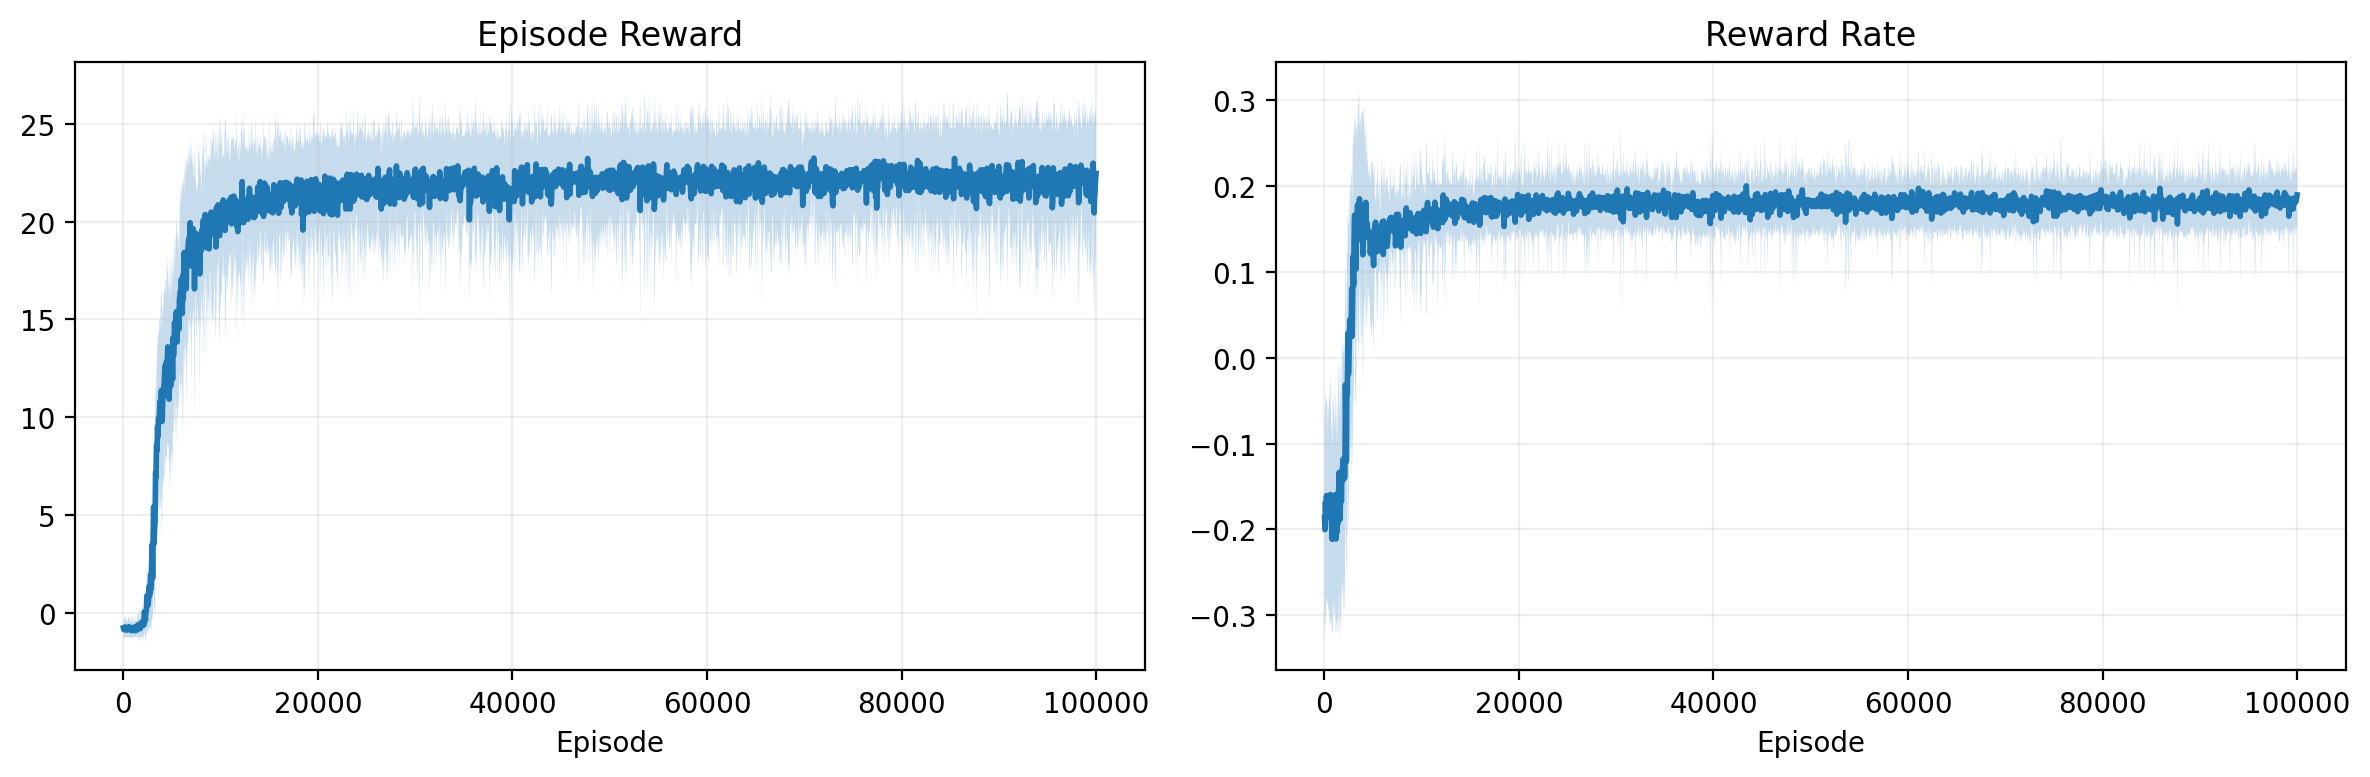
\includegraphics[width=0.92\linewidth]{images/EpisodicObjectivePPO.png}
    \caption[PPO with the episodic objective on Snake $5\times5$]{PPO trained
    on Snake $5\times5$ with the standard \emph{episodic} objective (the GAE
    done-mask left in place, so advantages do not cross episode boundaries).
    Left: total reward per episode; right: reward per step. Both curves are
    smoothed running averages over training ($100{,}000$ episodes), and the
    shaded band shows the spread of the raw per-episode values around the
    smoothed mean. Episode reward plateaus at roughly $22$ while the reward
    rate settles at $\approx 0.18$.}
    \label{fig:ppo-episodic}
\end{figure}

\begin{figure}[H]
    \centering
    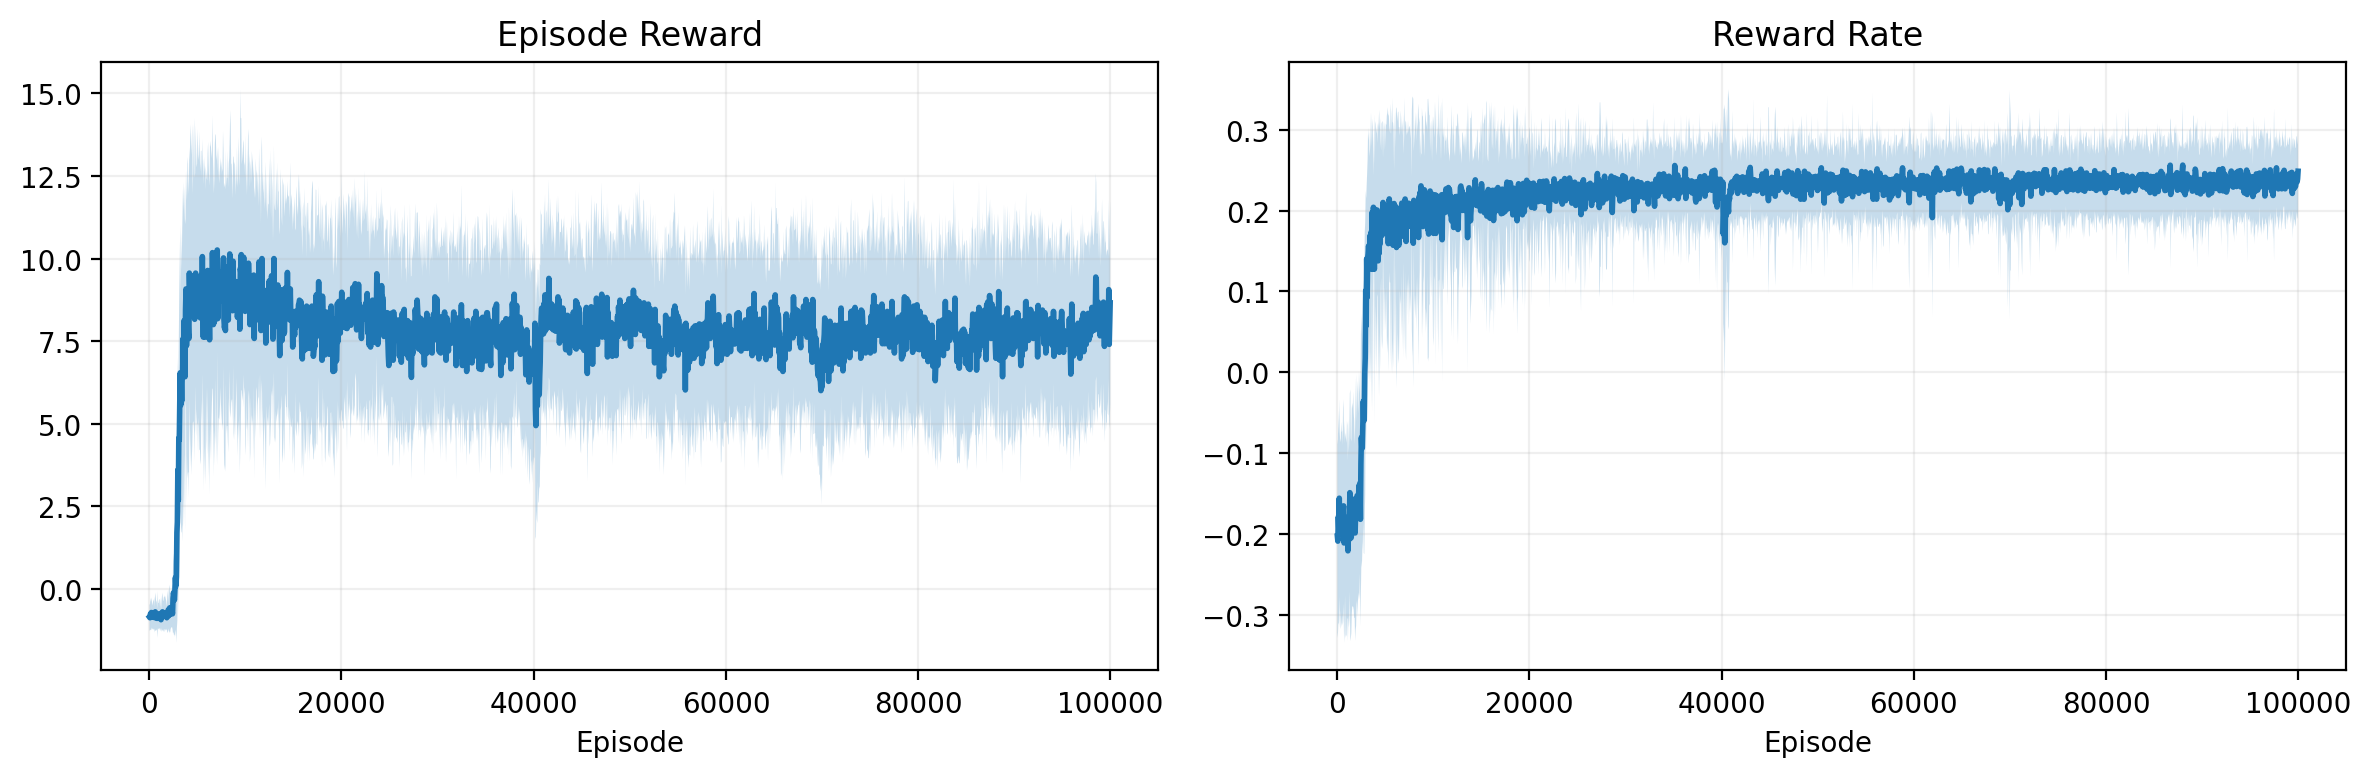
\includegraphics[width=0.92\linewidth]{images/ContinuousObjectivePPO.png}
    \caption[PPO with the continuing objective on Snake $5\times5$]{PPO
    trained on Snake $5\times5$ with the \emph{continuing} objective, no difference is made for terminal states, so the bootstrap and advantage
    recursion run through resets and the agent optimizes the uninterrupted
    reward stream, the same objective faced by the spiking agents. Axes and
    smoothing as in Figure~\ref{fig:ppo-episodic}. Relative to the episodic
    objective the picture inverts: episode reward plateaus far lower, at
    roughly $8$, while the reward rate rises to $\approx 0.24$, above the
    $\approx 0.18$ of the episodic agent. Each objective attains the higher
    value on the metric it actually optimizes.}
    \label{fig:ppo-continuous}
\end{figure}


The episodic and continuing objectives differ in exactly on the treatment of the
terminal transition in the advantage estimate, where the continuing variant lets the value
bootstrap across the episode boundary while the episodic variant masks it. Provided the critic
is reasonably accurate, how far this single difference propagates back into a trajectory is
largely governed by the value horizon $1/(1-\gamma)$. At $\gamma=0.99$ that horizon is roughly
$100$ steps, comparable to the length of a Snake episode, so the boundary treatment can reshape
the advantages of a large fraction of every trajectory. The two objectives then tend to pursue
different fixed points, one accumulating per-episode return and the other reward per step, and
the two performance metrics separate and can even move in opposite directions. At $\gamma=0.5$
the horizon shrinks to about $2$ steps, so the influence of the terminal transition decays
within a few steps and rarely reaches the body of an episode; masking it or not then makes
little practical difference, the episodic and continuing updates become nearly indistinguishable,
and the objectives, together with both metrics, largely converge. This reasoning does rest on the
value function being learned well enough for the bootstrap to behave as intended, an assumption we
expect to hold here because Snake $5\times5$ is predictable enough for the critic to be accurate;
in a task where the critic remained poor the picture could be less clean. Under that same
assumption the decoupled $\lambda=0.8$ would not, on its own, be expected to reopen the gap, as
discussed in Section~\ref{sec:practical-lambda}, it is primarily $\gamma$ that shapes \emph{what} is being optimized and hence
whether the episodic and continuing formulations differ appreciably. Were the critic largely
uninformative this separation would blur, and $\lambda$ could begin to influence the effective
objective; that this does not appear to happen here is itself consistent with the critic being
accurate on a task as predictable as Snake with the described rewards.

This also fixes the level at which the two curves meet. At $\gamma=0.5$ neither extreme strategy
is reachable, neither the long-survival behavior that maximizes per-episode return at
$\gamma=0.99$ (episode reward $\approx 22$) nor the most efficient reward-per-step policy
(reward rate $\approx 0.24$); a two-step horizon simply cannot represent either. Both objectives
instead settle on the same short-horizon compromise, an episode reward of about $13$ and a reward
rate of about $0.2$. Crucially, this is the \emph{same} $\gamma$ and $\lambda$ used by the
spiking rules, and the continuing PPO run lands essentially where symmetric e-prop does
(Section~\ref{sec:snake_lambda_comparison}). A strong gradient-based optimizer given the identical
short-horizon objective therefore reaches the same operating point as the local spiking rule,
which indicates that the spiking results are limited not by their credit-assignment machinery but
by the short objective horizon itself. This suggests that the headroom toward the higher reward rate seen at
$\gamma=0.99$ in this particular problem is recovered by lengthening the value horizon, that is by increasing $\gamma$.


\begin{figure}[H]
    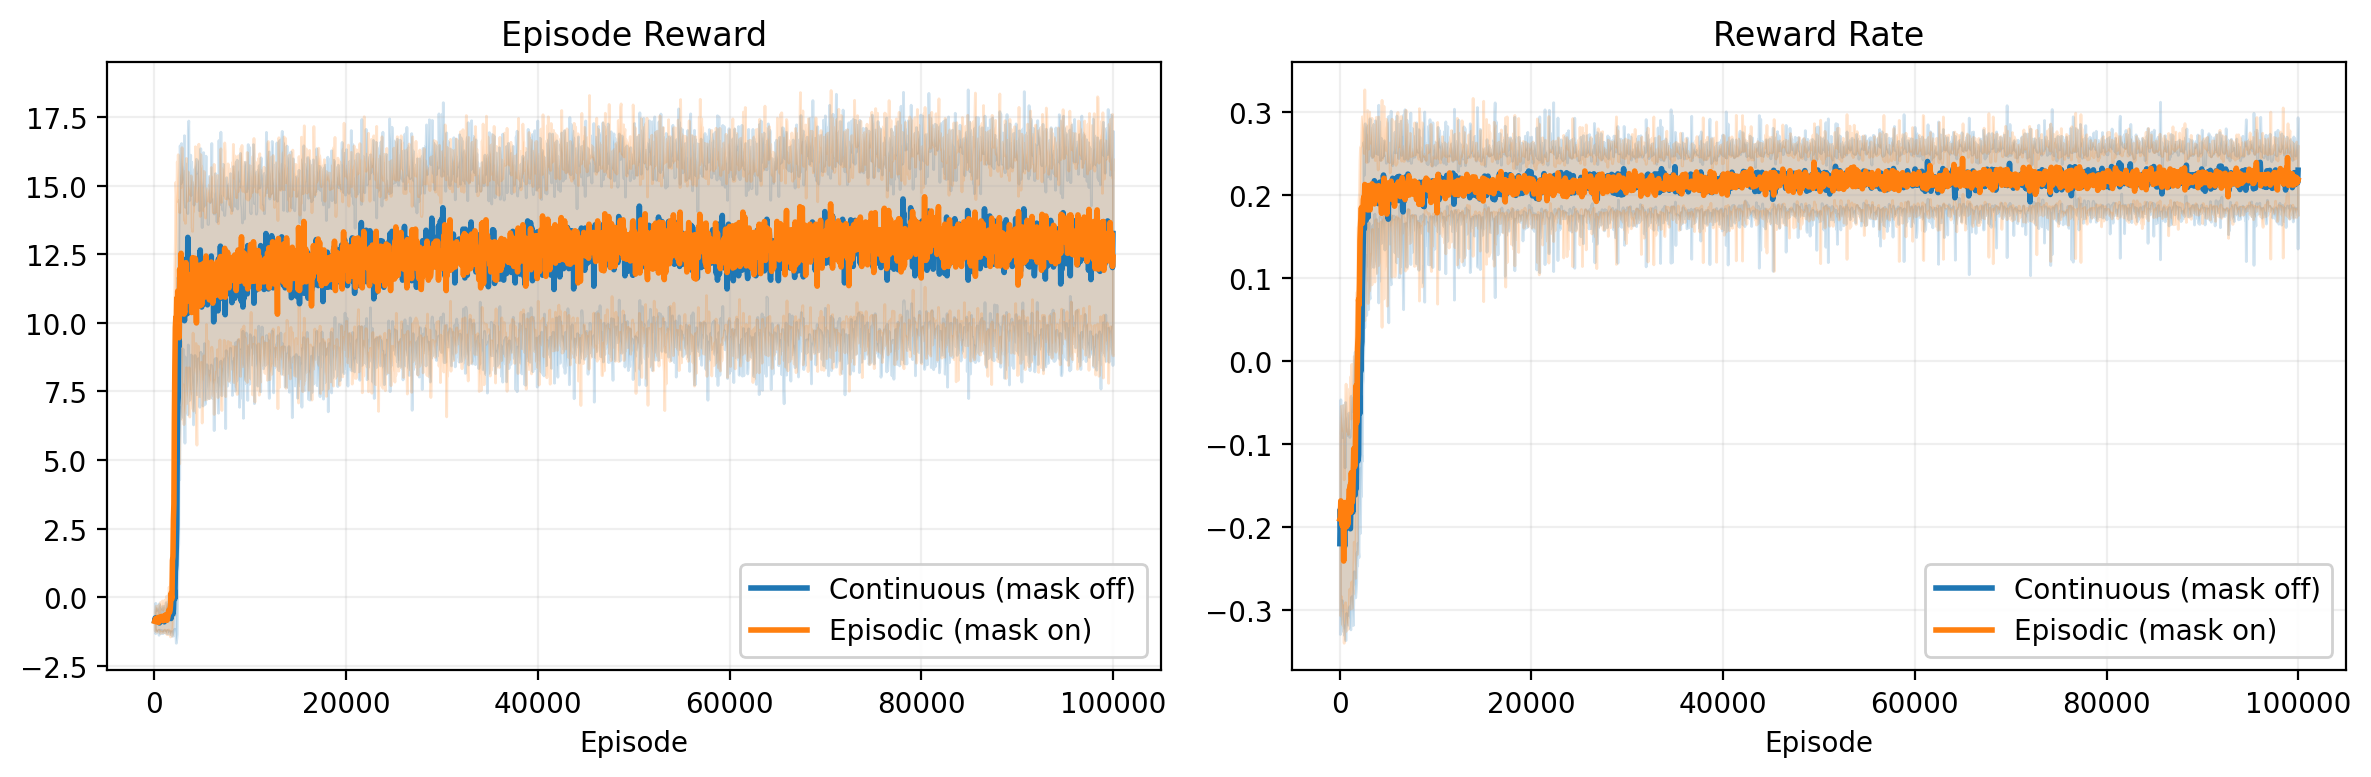
\includegraphics[width=\linewidth]{images/PPOComparison.png}
    \caption[Episodic vs.\ continuing PPO objective at $\gamma=0.5$, $\lambda=0.8$]{%
        PPO on Snake $5\times5$ under the episodic (terminal mask \emph{on}) and
        continuing (terminal mask \emph{off}) objectives, both with the decoupled
        setting $\gamma=0.5$, $\lambda=0.8$, overlaid on shared axes. \emph{Left:}
        episode reward. \emph{Right:} reward rate. Solid lines are the running mean
        and shaded bands the standard deviation across runs. In contrast to the
        $\gamma=0.99$ runs of Figures~\ref{fig:ppo-episodic} and~\ref{fig:ppo-continuous},
        the two objectives now nearly coincide on \emph{both} metrics.}
    \label{fig:ppo-episodic-vs-continuous}
\end{figure}

\section{Symmetric E-prop Dominance and Failure Case on Snake}
\label{sec:symmetric-failure}
\begin{figure}[H]
    \centering
    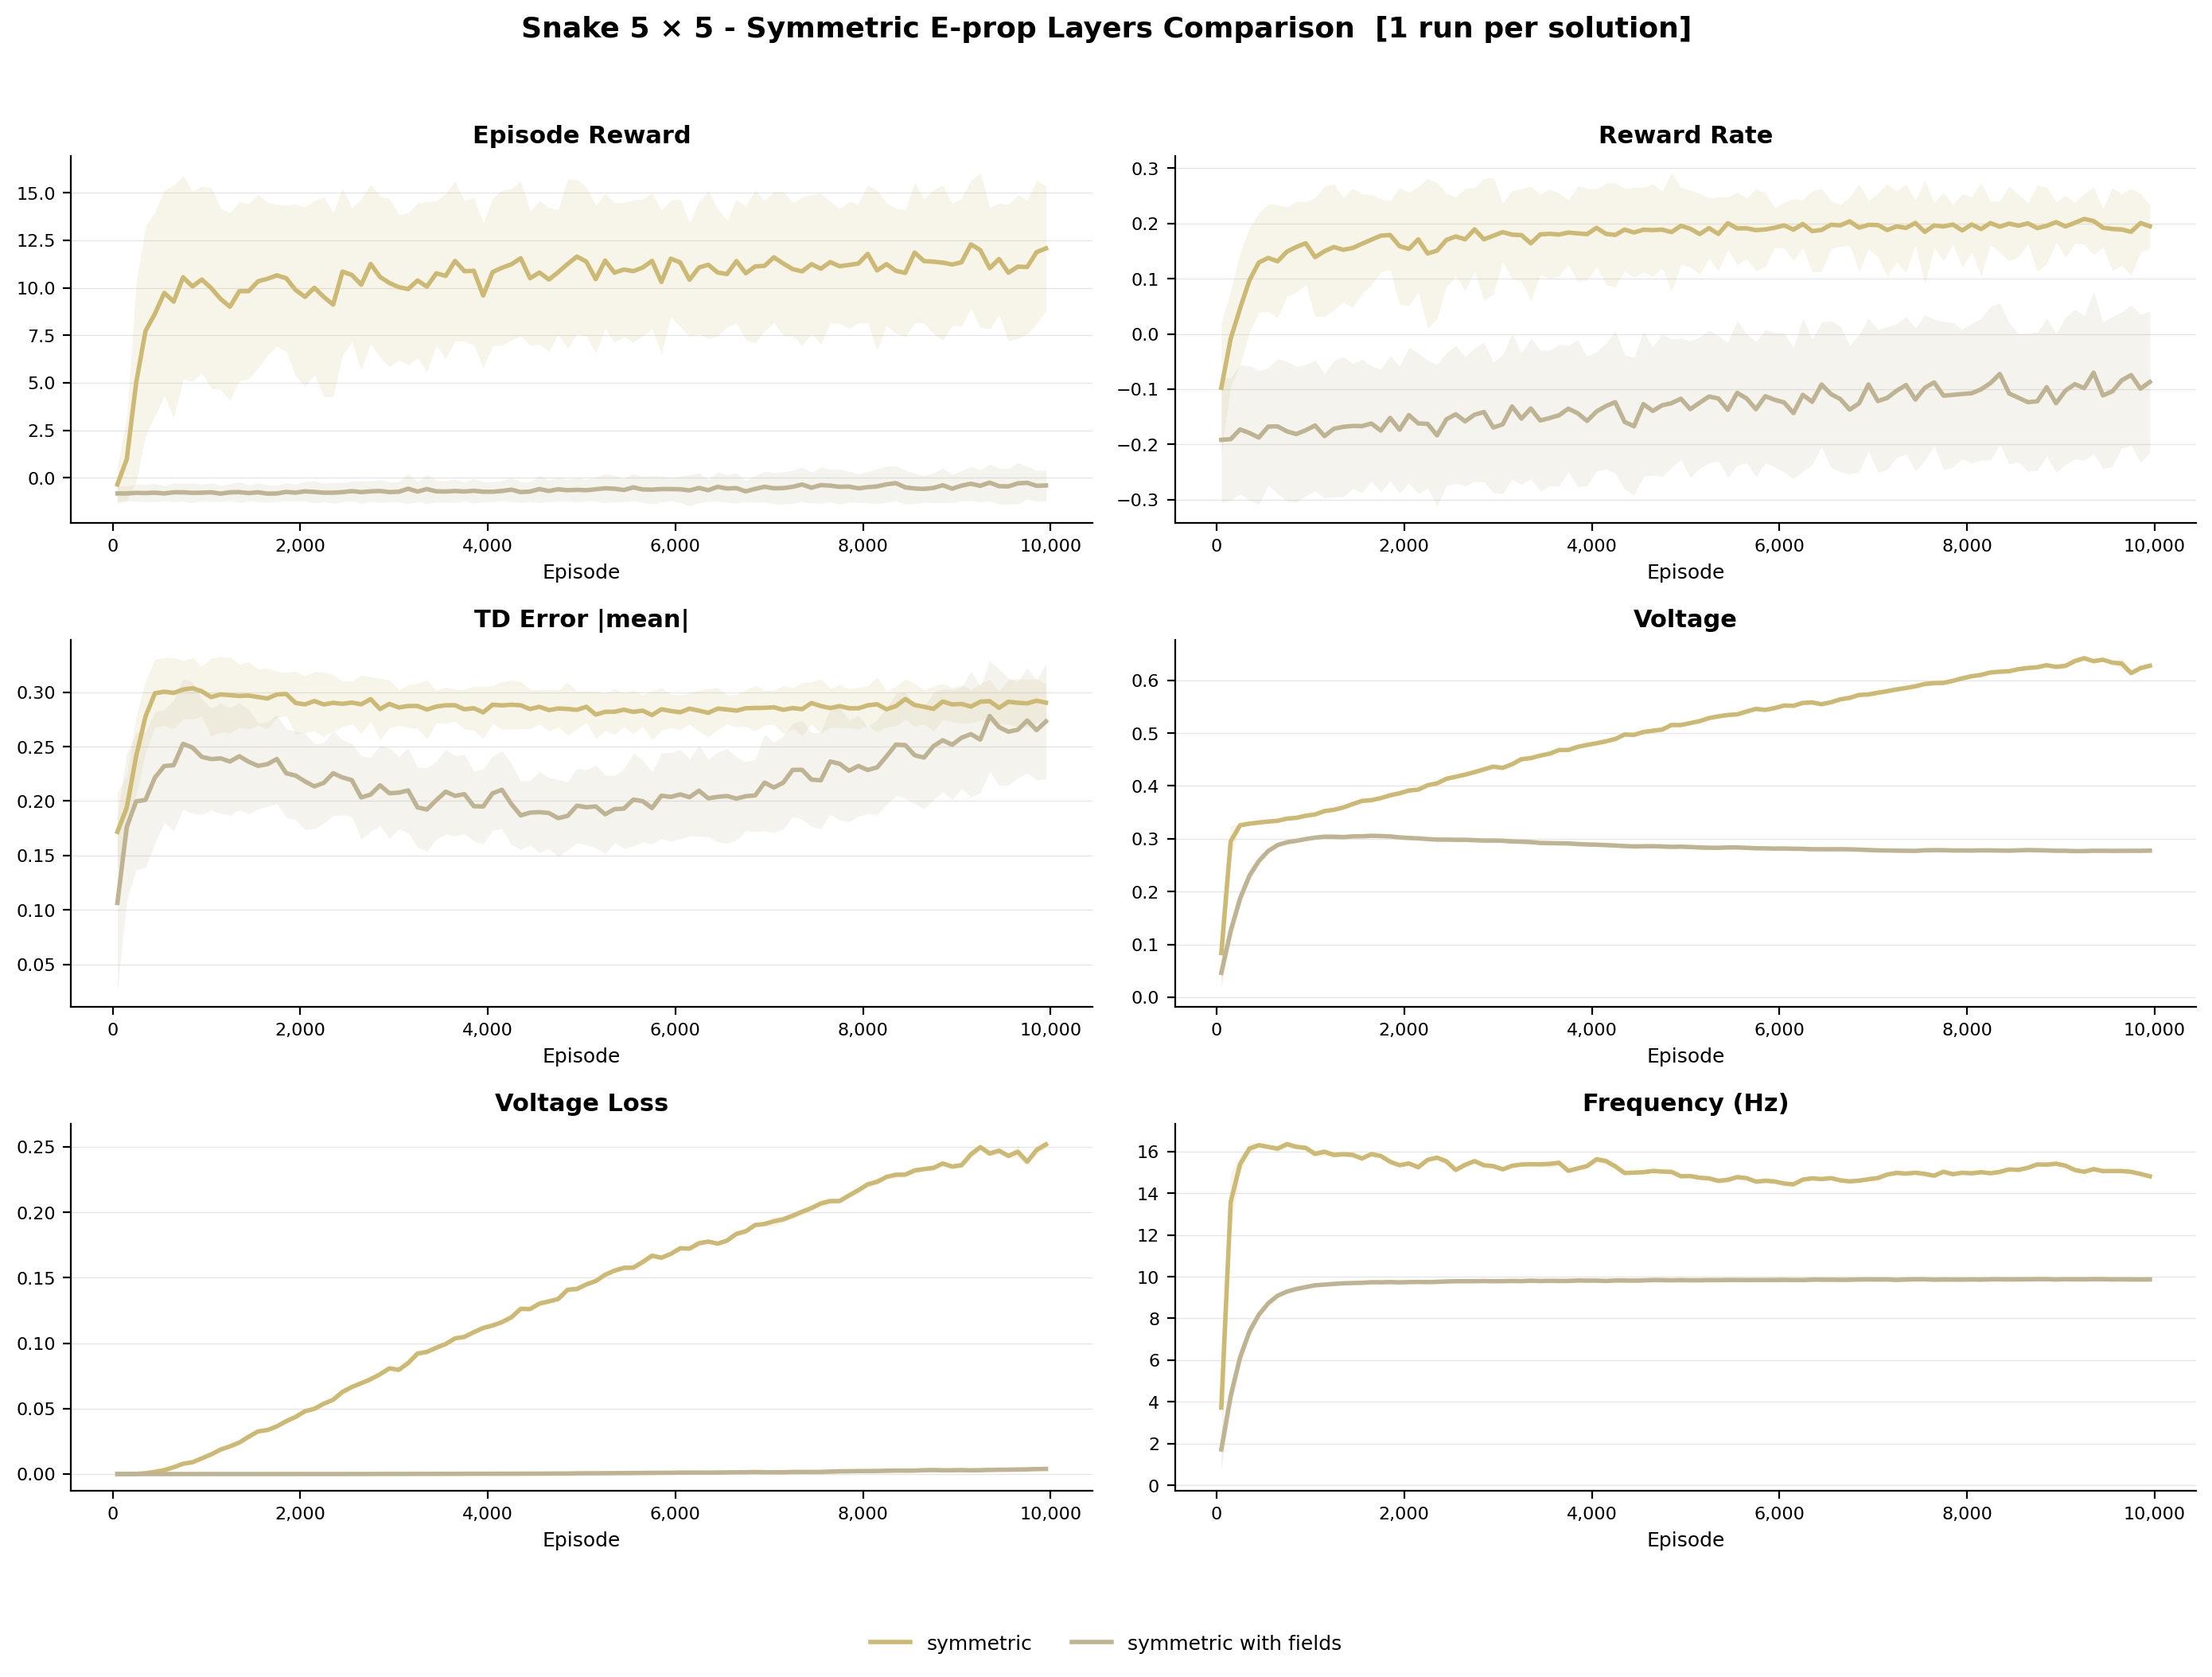
\includegraphics[width=1\linewidth]{images/SnakeSymmetric.png}
    \caption[Symmetric e-prop: with vs.\ without field layers]{Symmetric e-prop on Snake $5\times5$, with and without the per-head field layers
    (one run per configuration). Each panel tracks a quantity over $10{,}000$ episodes:
    episode reward, reward rate, mean absolute TD error, mean membrane voltage,
    voltage-regularization loss, and mean firing frequency (Hz). The plain symmetric variant
    attains the higher episode reward and reward rate together with the most favorable
    voltage and frequency statistics, whereas adding the value- and policy-field layers
    (\emph{symmetric with fields}) drives reward to near zero. The drop coincides with the
    longer causal path between input and output introduced by the field layers, which
    symmetric e-prop is unable to assign credit across reliably.}
    \label{fig:symmetric-layers}
\end{figure}
Of the configurations considered in this work, symmetric e-prop produces the strongest
overall behavior on Snake $5\times5$. As shown in Figure~\ref{fig:symmetric-layers}, it
converges to the highest episode reward and reward rate, and does so while maintaining the
most favorable voltage and frequency statistics, indicating a stable and well-regulated
spiking regime.

This advantage disappears as soon as the per-head field layers for the policy and value
outputs are introduced. The \emph{symmetric with fields} configuration suffers an absolute
drop in performance, with episode reward collapsing to near zero. The decisive factor is
the causal path length between input and output: the field layers lengthen this path, and
because the feedback weights of symmetric e-prop are tied to the forward output weights, the
credit assigned to non-connected neurons disappears. A
change that should be benign, namely adding expressive capacity to the read-out, instead breaks learning entirely.

The aggregate curves alone cannot tell us how the two configurations differ in behavior, only that they do. To understand what is actually lost when the field layers are introduced, Figures ~\ref{fig:qualitative_symmetric} and~\ref{fig:qualitative_symmetric_fields} examine a single representative episode from each configuration, revealing that the value function and policy both lose their structure entirely.

\begin{figure}[H]
    \centering
    \begin{subfigure}{0.538\linewidth}
        \centering
        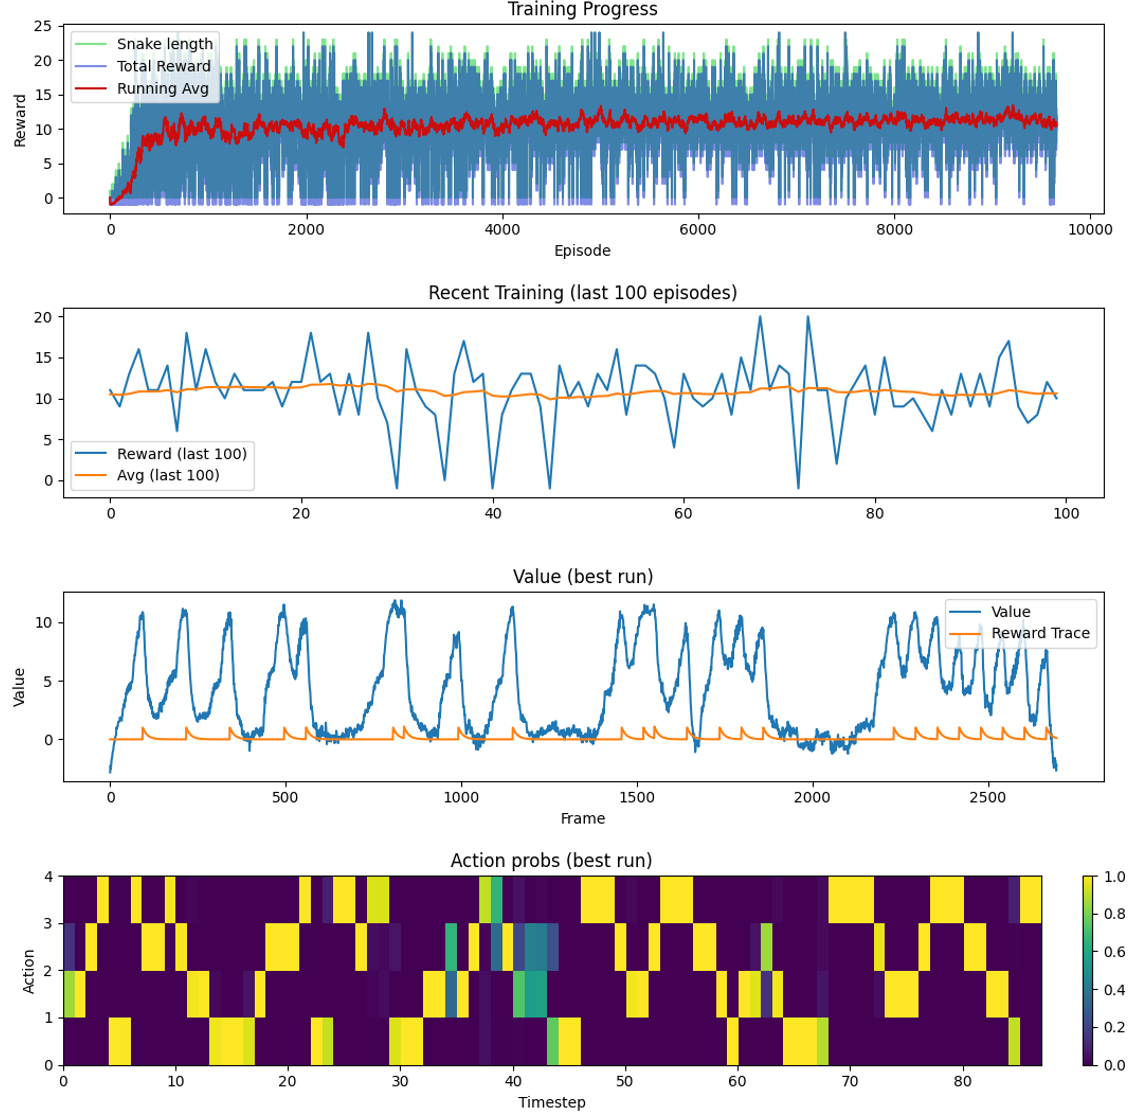
\includegraphics[width=\linewidth]{QualitativeSymmetric.png}
        \caption{Qualitative Symmetric}
        \label{fig:qualitative_symmetric}
    \end{subfigure}
    \hfill
    \begin{subfigure}{0.454\linewidth}
        \centering
        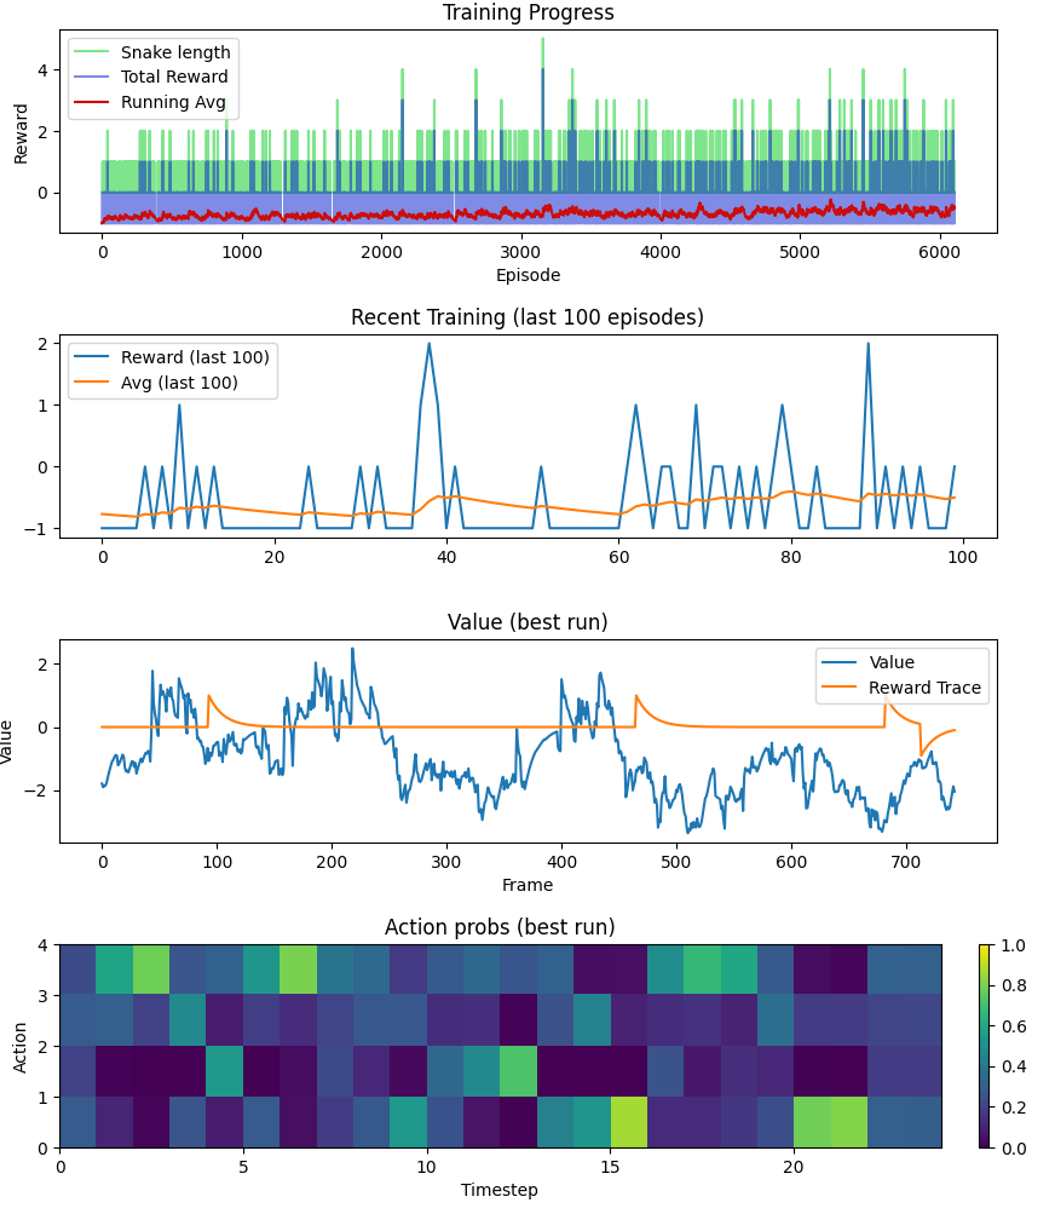
\includegraphics[width=\linewidth]{QualitativeSymmetricWithFields.png}
        \caption{Qualitative Symmetric With Fields}
        \label{fig:qualitative_symmetric_fields}
    \end{subfigure}
    
    \caption[Qualitative symmetric e-prop, field layers ablation]{Qualitative comparison of symmetric e-prop without (a) and with (b) the
    per-head field layers on Snake $5\times5$. From top to bottom each column shows: the
    training progress over all episodes (snake length, total reward, and running average);
    the reward over the most recent $100$ episodes against its running mean; the value
    estimate $V_t$ against the reward trace for the best run; and a heat map of the action
    probabilities through an episode. Without the field layers (a) the agent reaches
    greater snake lengths and rewards, its value trace is clearly structured, and its policy
    becomes close to deterministic (sharp light/dark bands); with the field layers (b)
    reward stays near zero, the value estimate is largely unstructured, and the policy
    remains diffuse.}
    \label{fig:qual-symmetric}
\end{figure}

Figure~\ref{fig:qual-symmetric} contrasts the two symmetric configurations on a single
representative run each. 
Without the field layers the agent produces long, reward-bearing episodes, a value
estimate with clear periodic structure, and an action distribution that sharpens into
near-deterministic choices. Once the field layers are introduced, the same diagnostics
degrade (reward collapses, the value trace loses its structure, and the policy stays
close to uniform), reinforcing the view that the longer credit path is responsible for the failure.

This failure is precisely what motivates the two alternative formulations studied in the
remainder of this chapter. The collapse is expected by the structure of symmetric e-prop, its feedback weights are
tied to the output weights, so if the majority of neurons do not have a connection to the output, then they do not receive any causal feedback information about the policy or value heads. This points to the property we
actually care about, namely a learning rule whose credit assignment scales gracefully with
causal path length. Two complementary ways of achieving it suggest themselves. The first is
to decouple the feedback pathway from the forward weights, as in random and adaptive e-prop,
where the learning signal is routed through fixed or independently learned feedback weights. 

The second, more radical option is to dispense with structured
feedback entirely, by treating each neuron as an independent stochastic actor
driven only by a global scalar signal and its own local action traces, changing the domain of the problem from a gradient routing problem to a noisy correlation problem.

\section{Distributed E-prop versus adaptive E-prop on Snake $5 \times 5$}
\label{sec:snake_comparison}

To assess how the different credit-assignment strategies behave on a fully observable
navigation task, we evaluate all variants on the Snake $5\times5$ problem over $10{,}000$
episodes, averaged over five independent runs. Figure~\ref{fig:snake_comparison} reports the
metrics introduced in Section~\ref{sec:reading-figures} for the configurations defined in
Table~\ref{tab:variant-naming}. In all cases the exploration variance $\sigma$ is held
fixed throughout training because the per-synapse variance
update of Section~\ref{subsec:exploration_variance} was not found to work reliably in practice and is
therefore excluded here. Shaded regions indicate the variability across runs.


\subsection{Comparison with $\lambda=0.8$}
\begin{figure}[h]
    \centering
    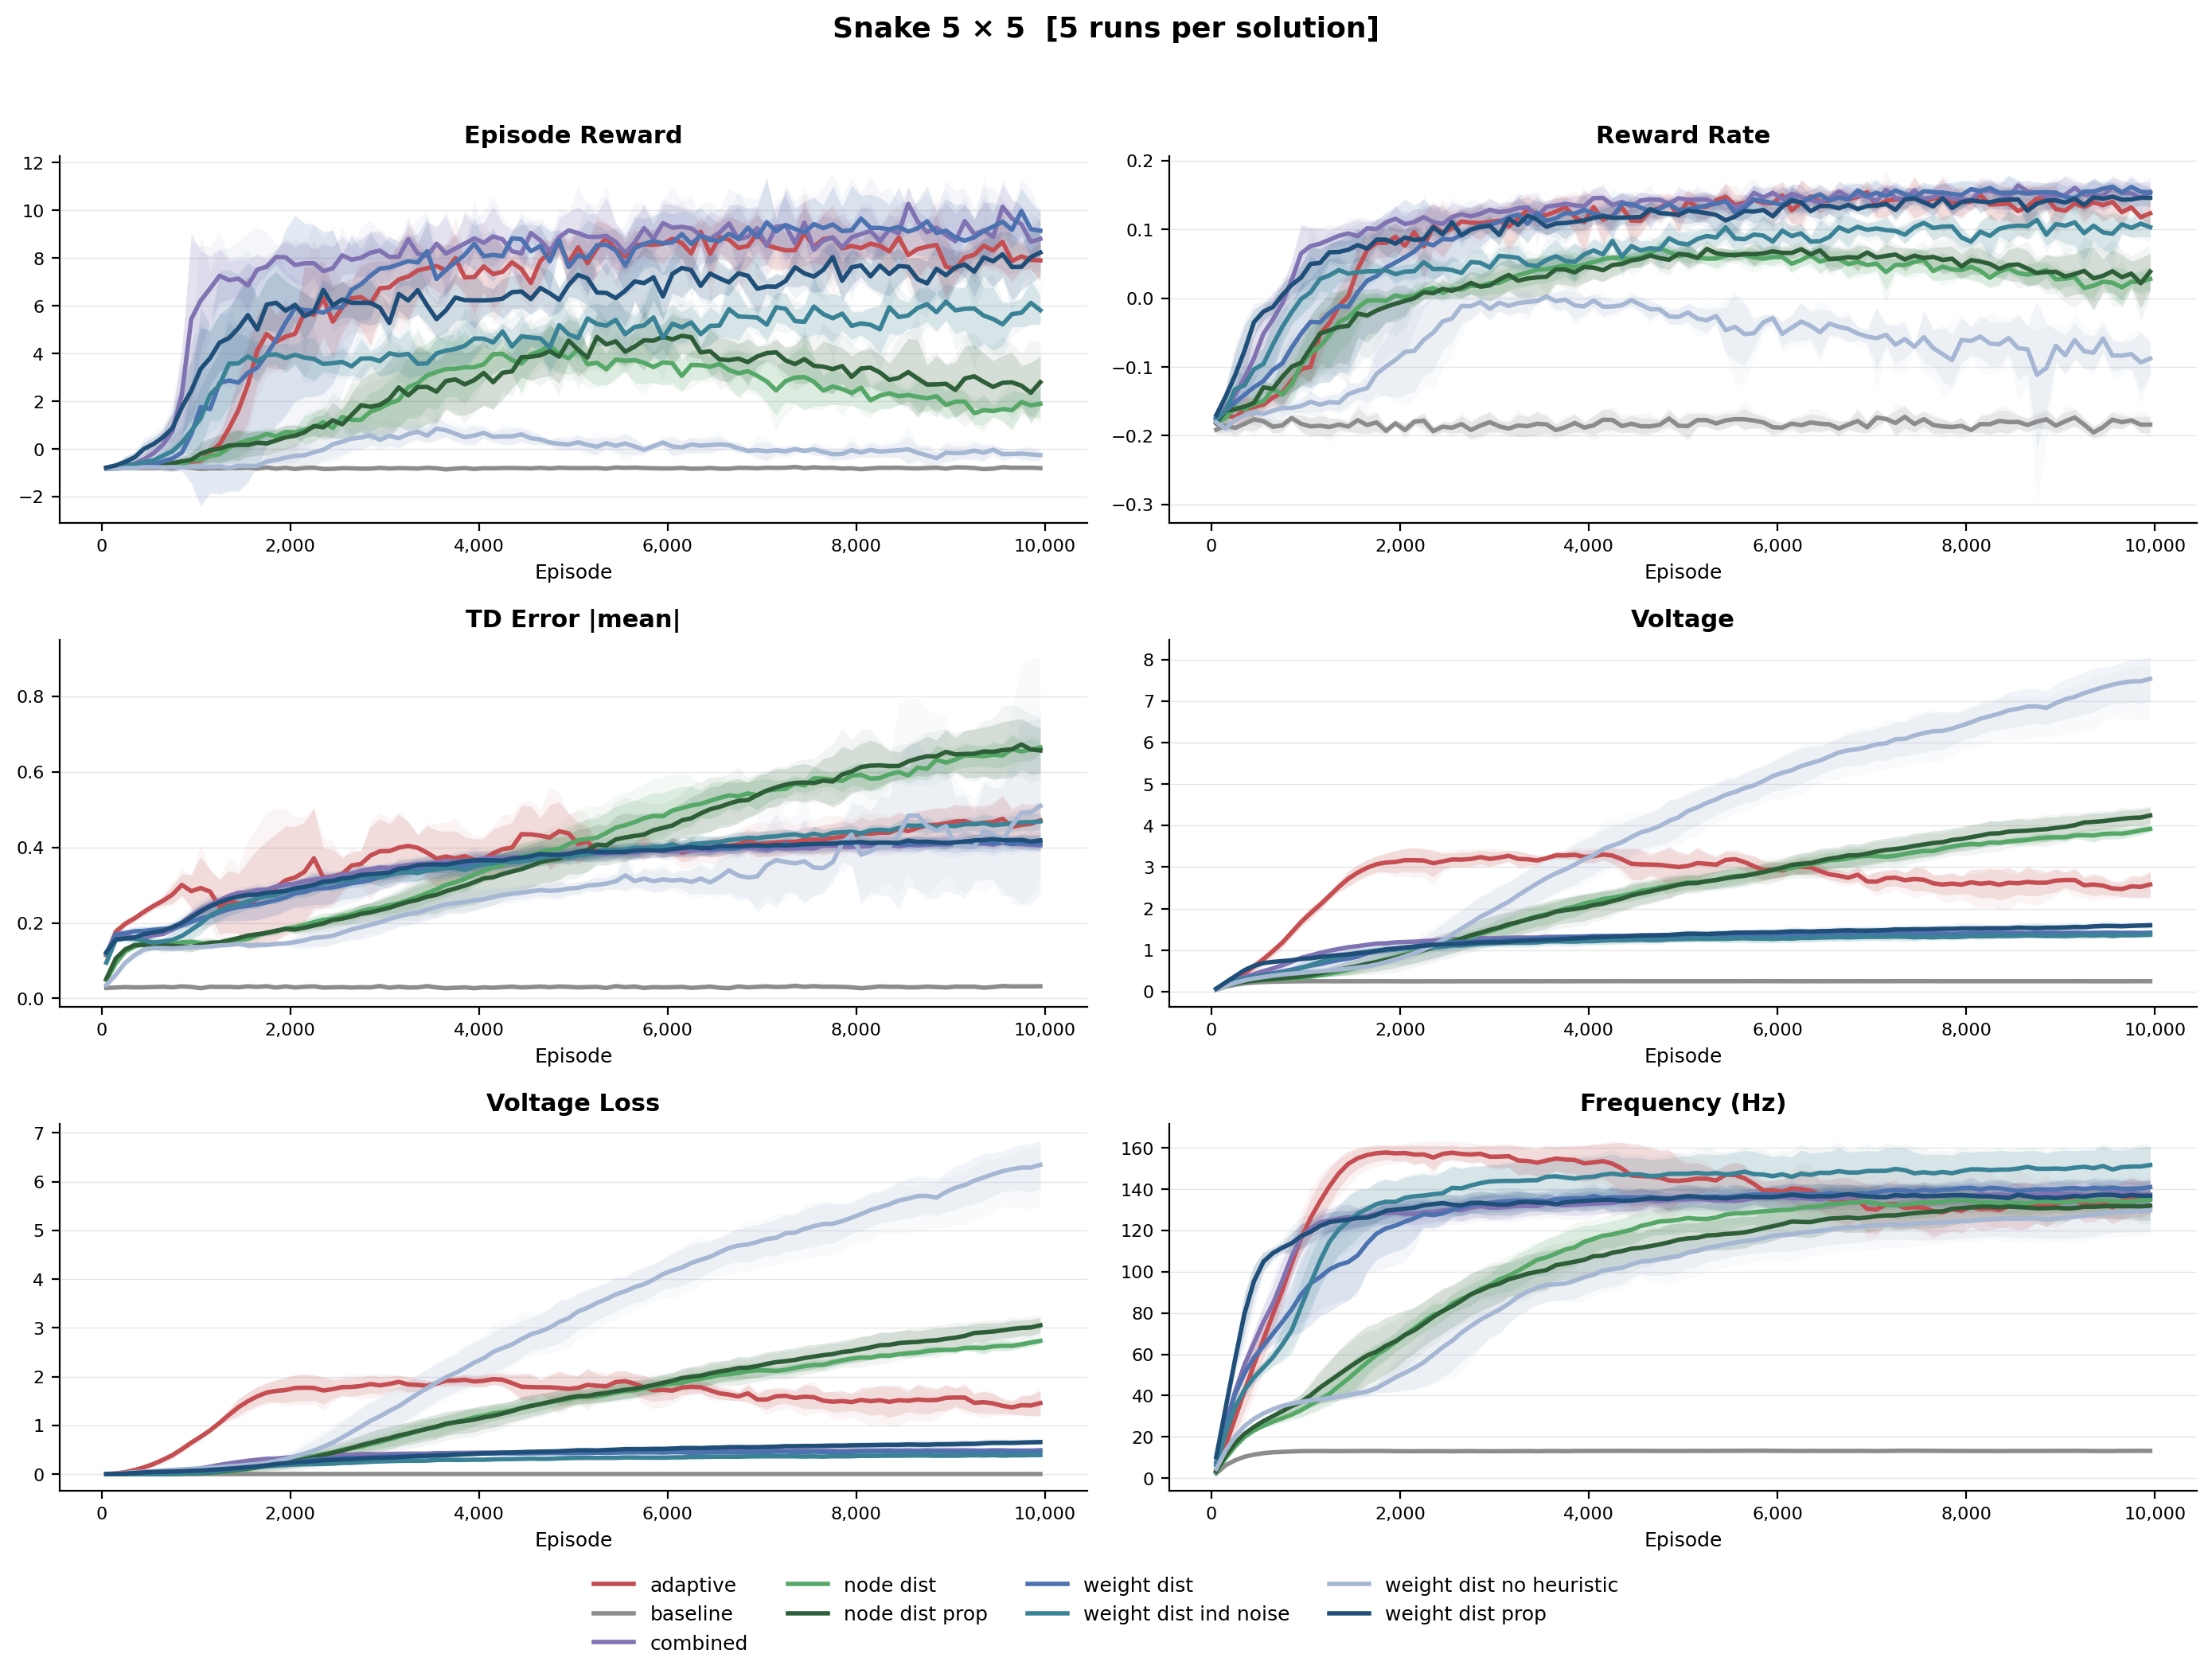
\includegraphics[width=\textwidth]{images/SnakeComparison.png}
    \caption[Credit-assignment variants on Snake $5\times5$]{Comparison of credit-assignment variants on the Snake $5\times5$ task over
    $10{,}000$ episodes. Each panel reports a different metric (episode reward, reward rate,
    mean absolute TD error, voltage, voltage loss, and frequency in Hz) for the configurations
    listed in the legend. Solid lines show the mean and shaded regions the variability across
    the five runs per configuration.}
    \label{fig:snake_comparison}
\end{figure}

\begin{figure}
    \centering
    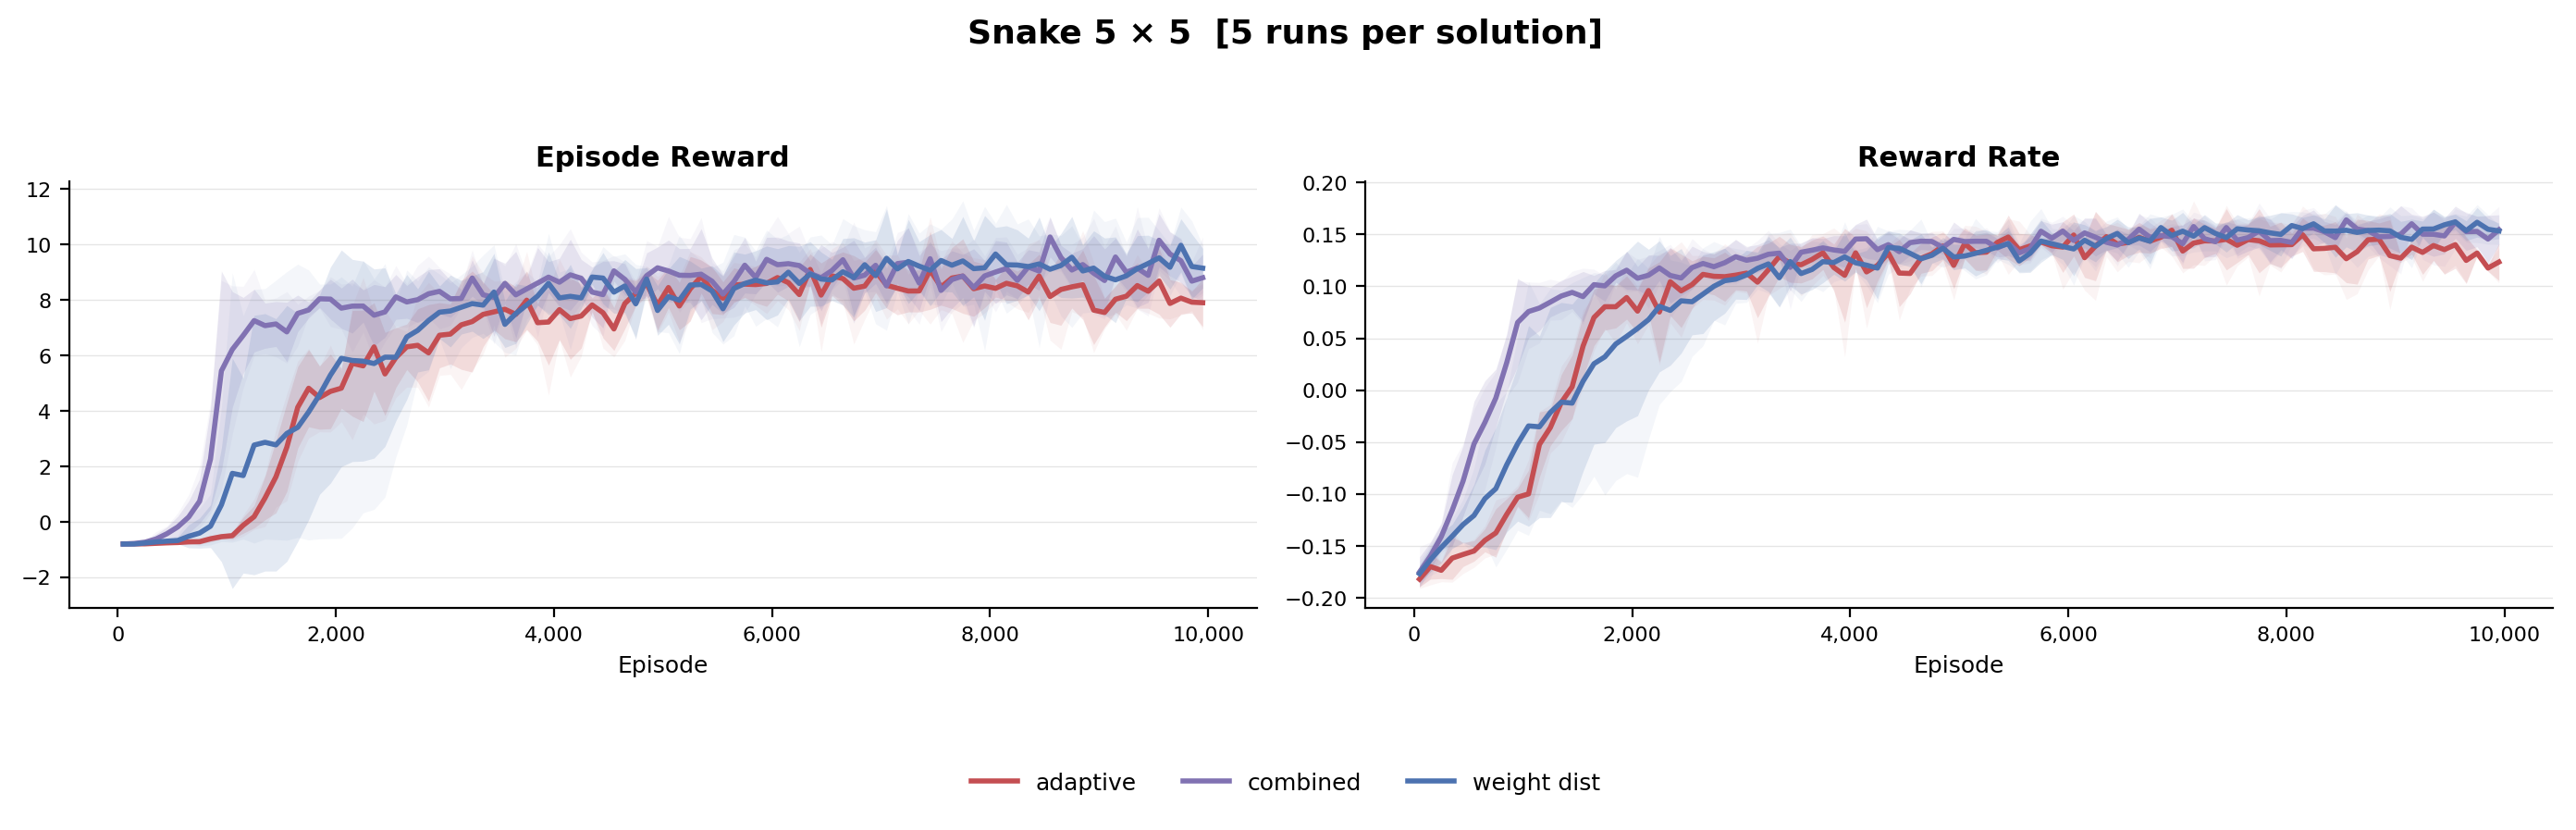
\includegraphics[width=1\linewidth]{SnakeTop3Comparison.png}
    \caption[Episode reward and reward rate, focused view (Snake, $5$ runs)]{%
    The two performance panels of Figure~\ref{fig:snake_comparison} (episode reward
    (left) and reward rate (right)) shown on their own for the three primary rules:
    adaptive (red), combined (purple) and weight dist (blue), on Snake $5\times5$
    with five independent runs each. Solid lines show the mean across runs and
    shaded bands the spread; the horizontal axis is the training episode. These
    panels are reproduced in isolation, away from the fuller diagnostic grid, so
    that the closely overlapping curves can be read more easily; the complete set of
    diagnostics and the accompanying discussion are given with
    Figure~\ref{fig:snake_comparison}.}
    \label{fig:placeholder}
\end{figure}


Before examining the individual metrics, it is worth stating the headline
result. Most variants learn the task successfully, converging to an episode
reward in the range of 8 to 10, but they differ substantially in how
quickly they do so, how stable their spiking dynamics are, and how well
their value functions track the actual return signal. The synaptic
perturbation variant \emph{weight dist} and the hybrid \emph{combined}
rule emerge as the strongest performers overall: \emph{combined} reaches
high reward faster than any other variant, while \emph{weight dist}
achieves the most stable final performance among the perturbation-based
rules, both maintaining low and well-regulated voltage throughout training.
Structured routing of the local policy signal has opposite effects depending
on the underlying estimator: it offers a modest improvement to the
neuron-perturbation variant \emph{node dist}, but disrupts the already
well-performing \emph{weight dist}, suggesting it is not universally
beneficial. The clearest failure case is \emph{weight dist no heuristic},
which demonstrates that the pseudo-derivative $\psi^t_j$ is not an optional
refinement but an essential component of the learning rule. The
\emph{adaptive} variant learns more slowly and shows signs of early
instability, but eventually reaches comparable performance. The following
analysis unpacks the mechanisms behind these differences metric by metric.

\paragraph{Episode Reward and Reward Rate.}

As a reference point, the \emph{baseline} configuration, in which only the output weights
are trained and the recurrent dynamics are left fixed, makes essentially no progress: its
episode reward stays close to zero throughout training and shows no discernible trend in
either direction. This confirms that solving the task requires shaping the recurrent dynamics
themselves, and that a trainable read-out on top of fixed recurrent activity carries
negligible learning capacity in this setting. It also provides a floor against which the
remaining variants can be read: any configuration that departs clearly from this flat
trajectory is, at minimum, propagating a usable learning signal into the recurrent weights.

Most variants learn the task successfully, converging to an episode reward in the range of
$8$ to $10$. The variant \emph{combined} stands out for its fast early improvement, reaching a
high reward well before the others, while \emph{weight dist} achieves the strongest
and most stable final performance among the perturbation-based variants. The \emph{adaptive} variant learns more slowly at first but eventually catches up to a comparable reward.

Two results within this comparison are particularly worth noting. First, \emph{weight dist} substantially outperforms \emph{node dist} despite the two using the same
number of independent stochastic perturbation sources, namely one Gaussian sample per
postsynaptic neuron in both cases (see Section~\ref{subsec:synaptic_perturbation}). The gap
between them is therefore not attributable to a variance difference, since variance is
approximately matched, and must instead stem from the bias introduced by the neuron-level
variant's shared credit: every synapse onto a given neuron receives an identical
perturbation trace regardless of whether that synapse's presynaptic neuron was actually
active, whereas the synaptic variant's effective perturbation $\varepsilon^t_{ji}z^t_i$ is
gated by presynaptic firing and therefore only contributes to a synapse's credit trace when
that synapse's presynaptic neuron actually fired. One plausible explanation for the size of
this gap, which we have not verified further and present here only as a working hypothesis,
is that this gating makes the synaptic perturbation trace inherently more reflective of the
network's actual causal activity pattern: a synapse is only perturbed, and therefore only
credited or discredited, at moments when it could plausibly have contributed to the
postsynaptic neuron's behavior, whereas the neuron-level trace accumulates noise
irrespective of which specific synapses were in a position to act. This remains a hypothesis, and a more direct test would be needed to confirm it.

Second, structured routing of the local policy signal has \emph{opposite} effects on the two
perturbation types. For the neuron-level estimator, \emph{node dist prop} performs
slightly better, on average over the five runs, than its unrouted counterpart \emph{node
dist}, suggesting that the additional structured information helps compensate, at least
partially, for the coarseness of the underlying credit signal. For the synaptic estimator,
however, structured routing is clearly detrimental: \emph{weight dist prop} learns quickly
at first, even appearing briefly competitive with \emph{weight dist}, but then stalls
for an extended period, and although it shows some recovery later in training it ends clearly
below the unrouted \emph{weight dist}. This asymmetry suggests that structured routing
is not uniformly beneficial, but instead interacts differently depending on how reliable the
underlying local estimator already is: it appears to help an estimator that is already biased
and has comparatively little to lose, while it appears to disrupt an estimator that was
already performing well, plausibly by introducing an additional, only partially aligned source
of signal that the optimization must reconcile with the existing perturbation-based update.

A further ablation isolates the role of the pseudo-derivative $\psi^t_j$ in the eligibility
trace. The \emph{weight dist no heuristic} configuration is identical to \emph{weight dist} except that it removes the surrogate-derivative factor $\psi^t_j$, retaining only the
filtered presynaptic spike train $\bar{z}^t_i$, with no postsynaptic
gating. Among the configurations that train the recurrent and input weights, it is the worst
performer by a wide margin, attaining the lowest episode reward and reward rate and falling
well short of every other recurrent learning variant. This suggests that the pseudo-derivative is not an
optional refinement but an essential component of the learning rule: by restricting credit to
moments when the postsynaptic neuron is close to its firing threshold, $\psi^t_j$ keeps the
perturbation-based update aligned with the network's causal activity, and without it the credit
signals degrade to the point where they are unable to train the network.

\paragraph{TD Error.}
Before discussing the curves themselves, it is worth being explicit about how much weight
this metric can bear. A value function that has learned a genuinely useful predictive representation need not produce
a smaller TD error than a flatter, less informative one: the magnitude of $\delta_t$ reflects
the moment-to-moment mismatch between the value estimate and a bootstrapped, trace-based
target, not the long-run accuracy of the prediction, and a critic that barely moves from a
constant baseline can trivially produce small errors against a slowly varying trace without
having learned anything useful. We therefore do not treat the TD error as a direct proxy for
critic quality in what follows. The one use we consider defensible, with some caution, is as a
coarse indicator of \emph{instability}: a TD error that grows steadily or fluctuates with
increasing magnitude over training is at least consistent with a critic whose internal
dynamics are drifting, even though a low or flat TD error cannot, by the
same logic, be read as positive evidence of a good critic. Even this weaker reading should be
treated with caution, which is precisely why we
complement this quantitative metric with the qualitative value-trace inspection introduced in Section~\ref{sec:value-traces}.

With that caveat in mind, we limit ourselves to comparative observations. The adaptive
variant shows signs of instability in its TD error early in training, with an initial rise
and noticeable fluctuation before it settles onto a plateau. This aligns with the qualitative
value traces we will see in \ref{fig:value-trace-progression-snake}, where adaptive e-prop appears to struggle more
than the perturbation variants with learning the value function. The perturbation-based variants
follow a visibly different profile, with a TD error that grows more gradually over the course
of training, though we do not read anything further into this beyond the difference in shape.
The synaptic variants \emph{weight dist} and \emph{combined} keep their TD error
comparatively low and stable throughout. Across all configurations we do not observe a runaway
explosion in the TD error, which is consistent with the caveat above: this metric is better
suited to flagging instability than to certifying the quality of a learned value function.

\paragraph{Voltage and Voltage Loss.}
The spiking dynamics again split along the same lines as the reward results, with the
node-perturbation and synaptic families behaving very differently. The two node-perturbation
variants, \emph{node dist} and \emph{node dist prop}, both show a continuously increasing
membrane voltage and voltage loss throughout training, drifting to the highest values among
the variants that learn the task. Structured routing makes little difference here: the routed
and unrouted versions track one another closely, so the prop variants are only marginally
increased relative to their base counterparts. The adaptive variant displays a characteristic
early surge in voltage that subsequently relaxes, settling back towards a moderate level. By
contrast, the synaptic variants \emph{weight dist} and \emph{weight dist prop}, together
with \emph{combined}, hold low and stable voltage and voltage loss across the entire run,
reflecting tightly controlled spiking activity. The clearest outlier is \emph{weight dist no
heuristic}: with the pseudo-derivative removed, its membrane voltage diverges, growing without
settling for the entire run and reaching values well beyond every other configuration.

\paragraph{Frequency.}
The firing frequency of all variants increases during training and converges to a broadly
similar band of roughly $130$ to $150$ Hz, which is very high, regardless of which credit-assignment strategy is
used. The \emph{adaptive} variant again
rises fastest and overshoots the eventual range early before settling, mirroring its early
voltage surge, whereas the node-perturbation variants approach the common range more gradually. The variant \emph{weight dist no heuristic} is no exception here, converging to the same high band as the
others, so frequency does little to distinguish it despite its poor reward and diverging voltage.


\begin{figure}[H]
    \centering
    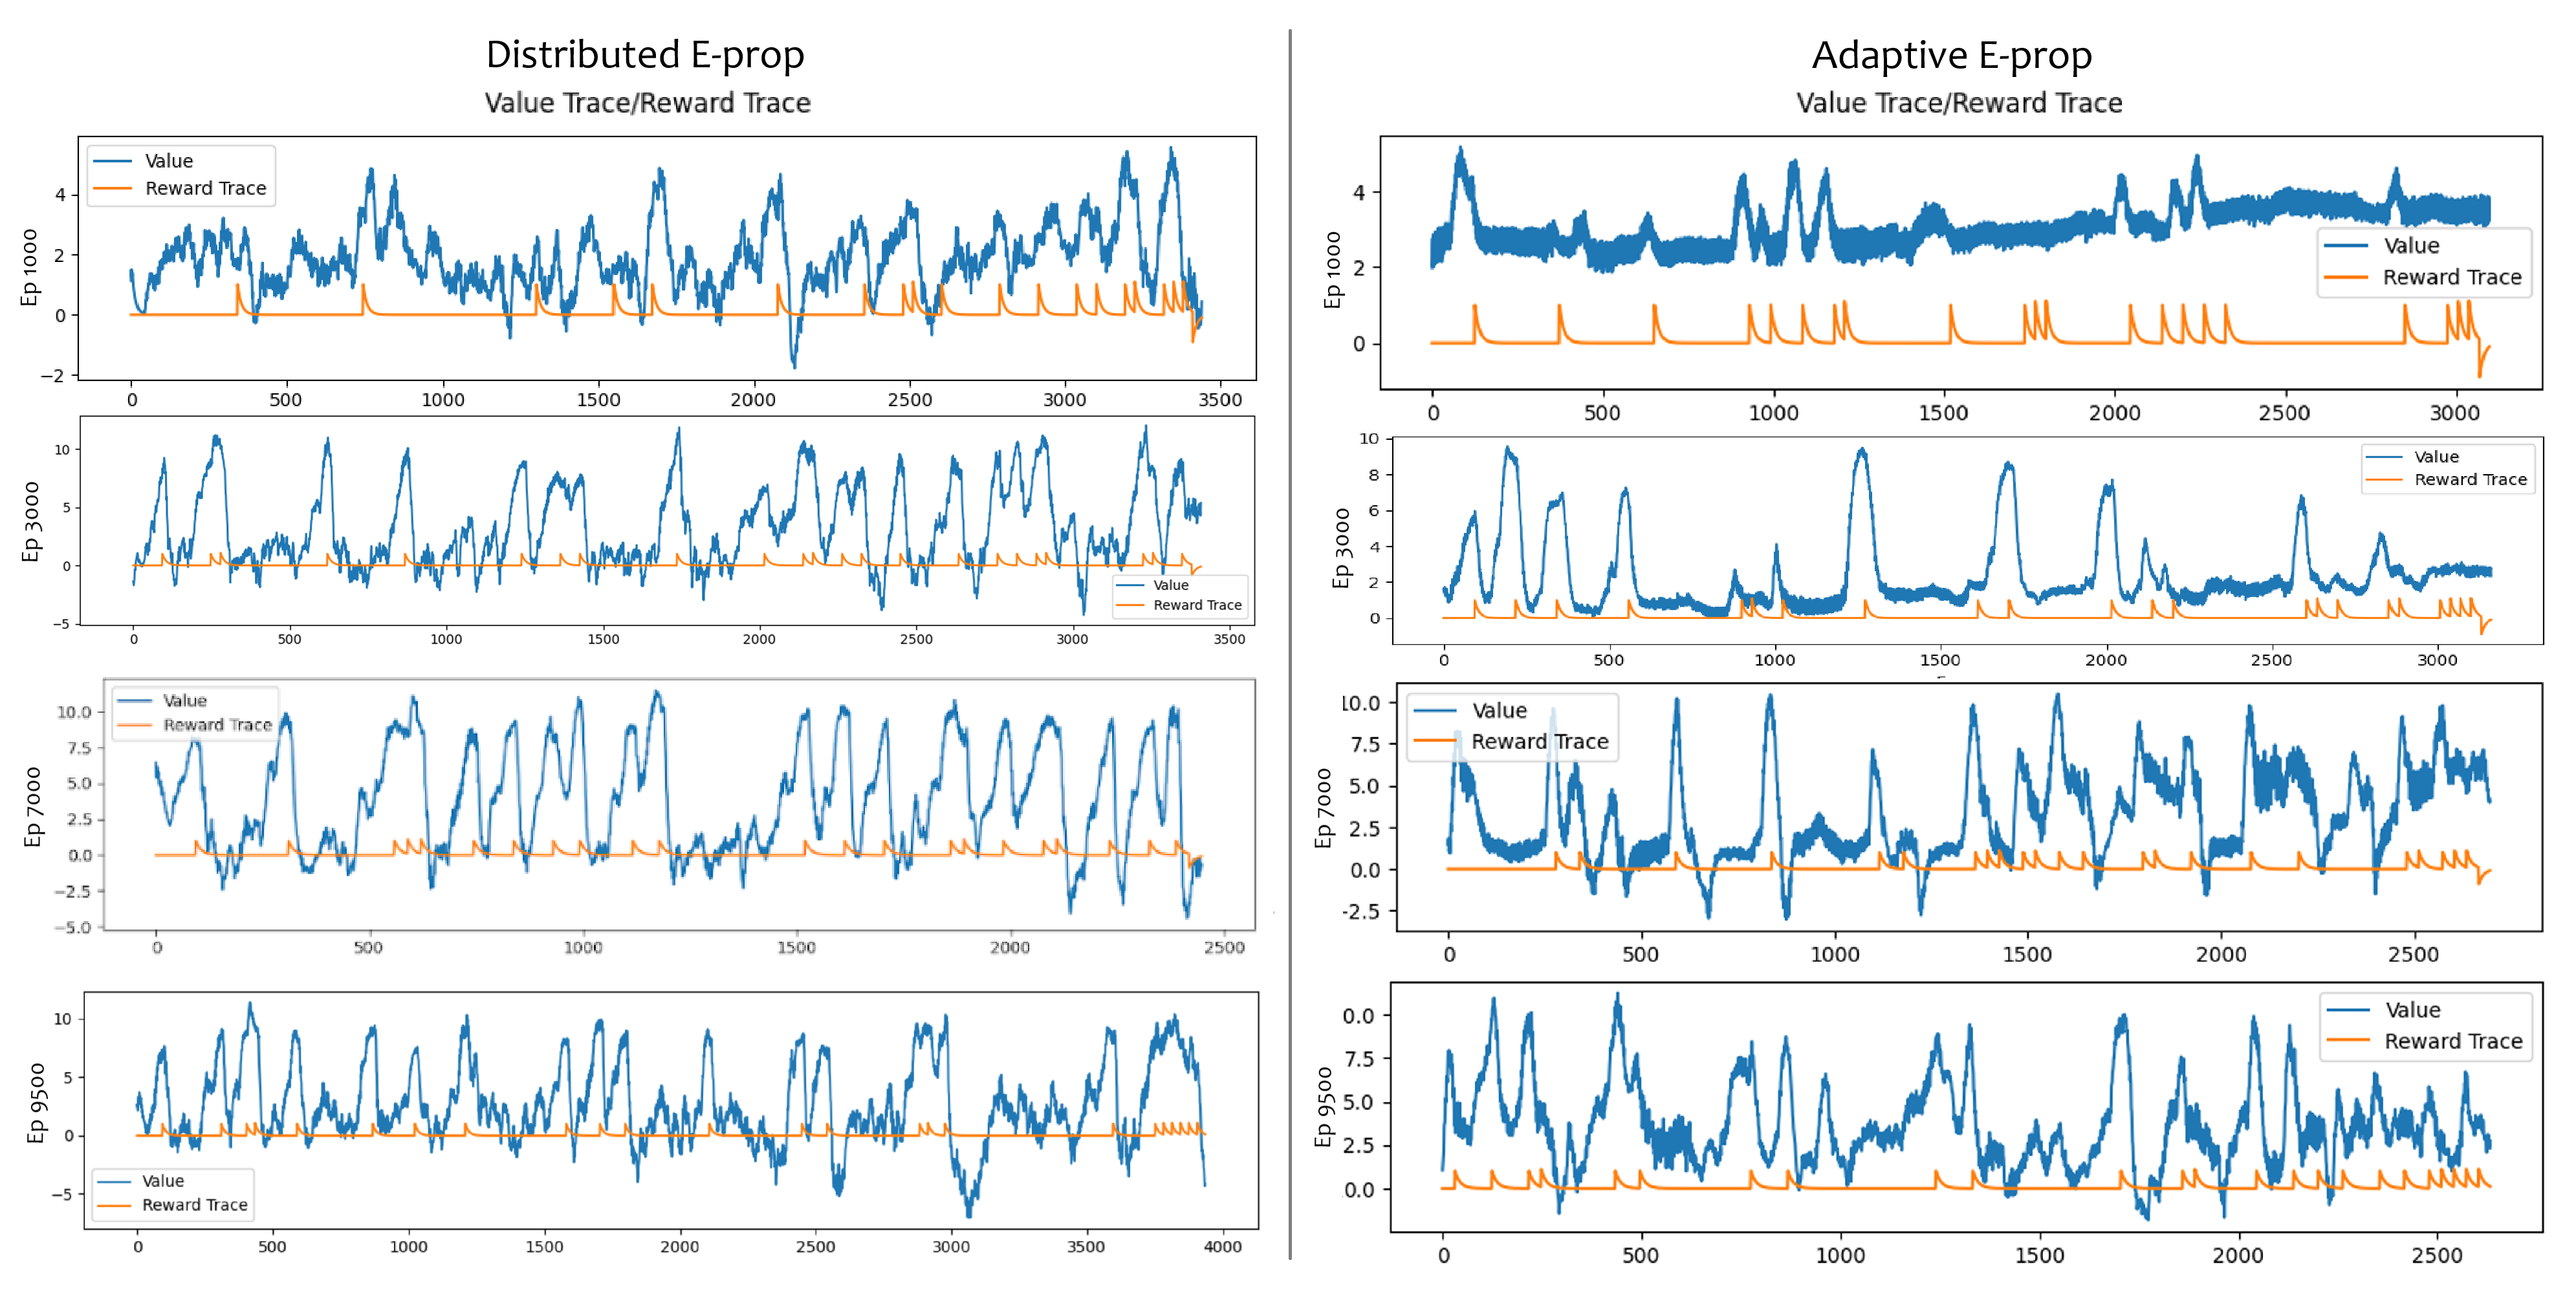
\includegraphics[width=1\linewidth]{images/SnakeValueTraceComparison.png}
    \caption[Value and reward traces on Snake]{%
    Value and reward traces for distributed e-prop (left) and adaptive e-prop
    (right) on Snake. The figure combines two distinct notions of time, which
    the axes deliberately keep separate. Reading down a column, each row is a
    snapshot taken at a different point in training (episodes $1000$, $3000$,
    $7000$ and $9500$ of the same run) so successive rows show how the value
    function develops as learning progresses; a column is not a single
    continuous trace. Reading across a panel, the horizontal axis is the
    frame number within a single game played at that checkpoint, and it necessarily
    restarts from zero in every panel; because games last for different numbers of
    frames, the panels span different frame counts and so differ in width. In every
    panel the blue curve is the critic's value estimate and the orange curve is the
    reward trace, whose spikes mark the frames at which reward is received. The
    vertical scales are independent from panel to panel, the magnitude of the
    learned value grows over training, and each panel is scaled to its own range so
    that the within-game structure remains visible.
    }
    \label{fig:value-trace-progression-snake}
\end{figure}

Read from top to bottom, Figure~\ref{fig:value-trace-progression-snake} shows how the relationship between the
value trace and the reward signal is expected to evolve as learning proceeds, following the
qualitative signature introduced in Section~\ref{sec:reading-figures}: an early value estimate
that tracks reward only loosely and without anticipation, gradually giving way to sharper,
structured excursions that lead reward events instead of trailing them, rising ahead of an
apple being collected and falling ahead of a collision. We use this progression throughout the
chapter to argue that a variant has learned a genuinely predictive value function.

A closer comparison between the two variants in Figure~\ref{fig:value-trace-progression-snake} reveals a
qualitative difference beyond this general progression. Although it is read from a single run
per variant, and is therefore illustrative, it is consistent across
the episodes shown. The value trace learned by distributed e-prop settles into a clean and
highly predictable shape, we can see how the estimate rises gradually, reaches a peak shortly before a reward
event, and then descends precisely at the moment the reward is received, closely tracking the
true timing of the underlying event. Adaptive e-prop takes considerably longer to adjust during
training, and even after extended learning it never develops this same predictive shape. Its
value trace remains comparatively noisier and less consistently timed, lacking the smooth
rise-and-fall structure that distributed e-prop shows in relation to reward delivery. This
contrast suggests that distributed e-prop arrives at a sharper and more temporally precise value
representation, while adaptive e-prop's critic remains comparatively underdeveloped within the
same training budget, consistent with the early instability seen in its TD error in Figure~\ref{fig:snake_comparison}.

\subsection{Lambda Comparison}
\label{sec:snake_lambda_comparison}

The experiments presented so far in this chapter have used a single fixed
value of the decay factor $\lambda$ from the TD($\lambda$) algorithm
throughout training. We now turn to the sensitivity of each learning rule
to this choice. As discussed in Section~\ref{sec:practical-lambda},
$\lambda$ sets the effective horizon, of order $1/(1-\lambda)$ steps, over
which a temporal-difference error is distributed back onto past
contributions, so small $\lambda$ concentrates credit near the present
action, while $\lambda$ close to 1 holds much earlier actions accountable,
at the cost of a higher-variance credit trace. This tradeoff is a property
of TD($\lambda$) in general, but how severely a given learning rule is
affected by it, and over what range of $\lambda$ it remains usable at all,
is an empirical question specific to how that rule constructs its update
from the credit trace. We examine this here on the Snake $5\times5$ task,
and return to it on the Pac-Man randomized layouts problem in
Section~\ref{sec:lambda_comparison}, since comparing the two will turn out
to be informative precisely because the two tasks produce different
answers.

\begin{figure}[htbp]
    \centering
    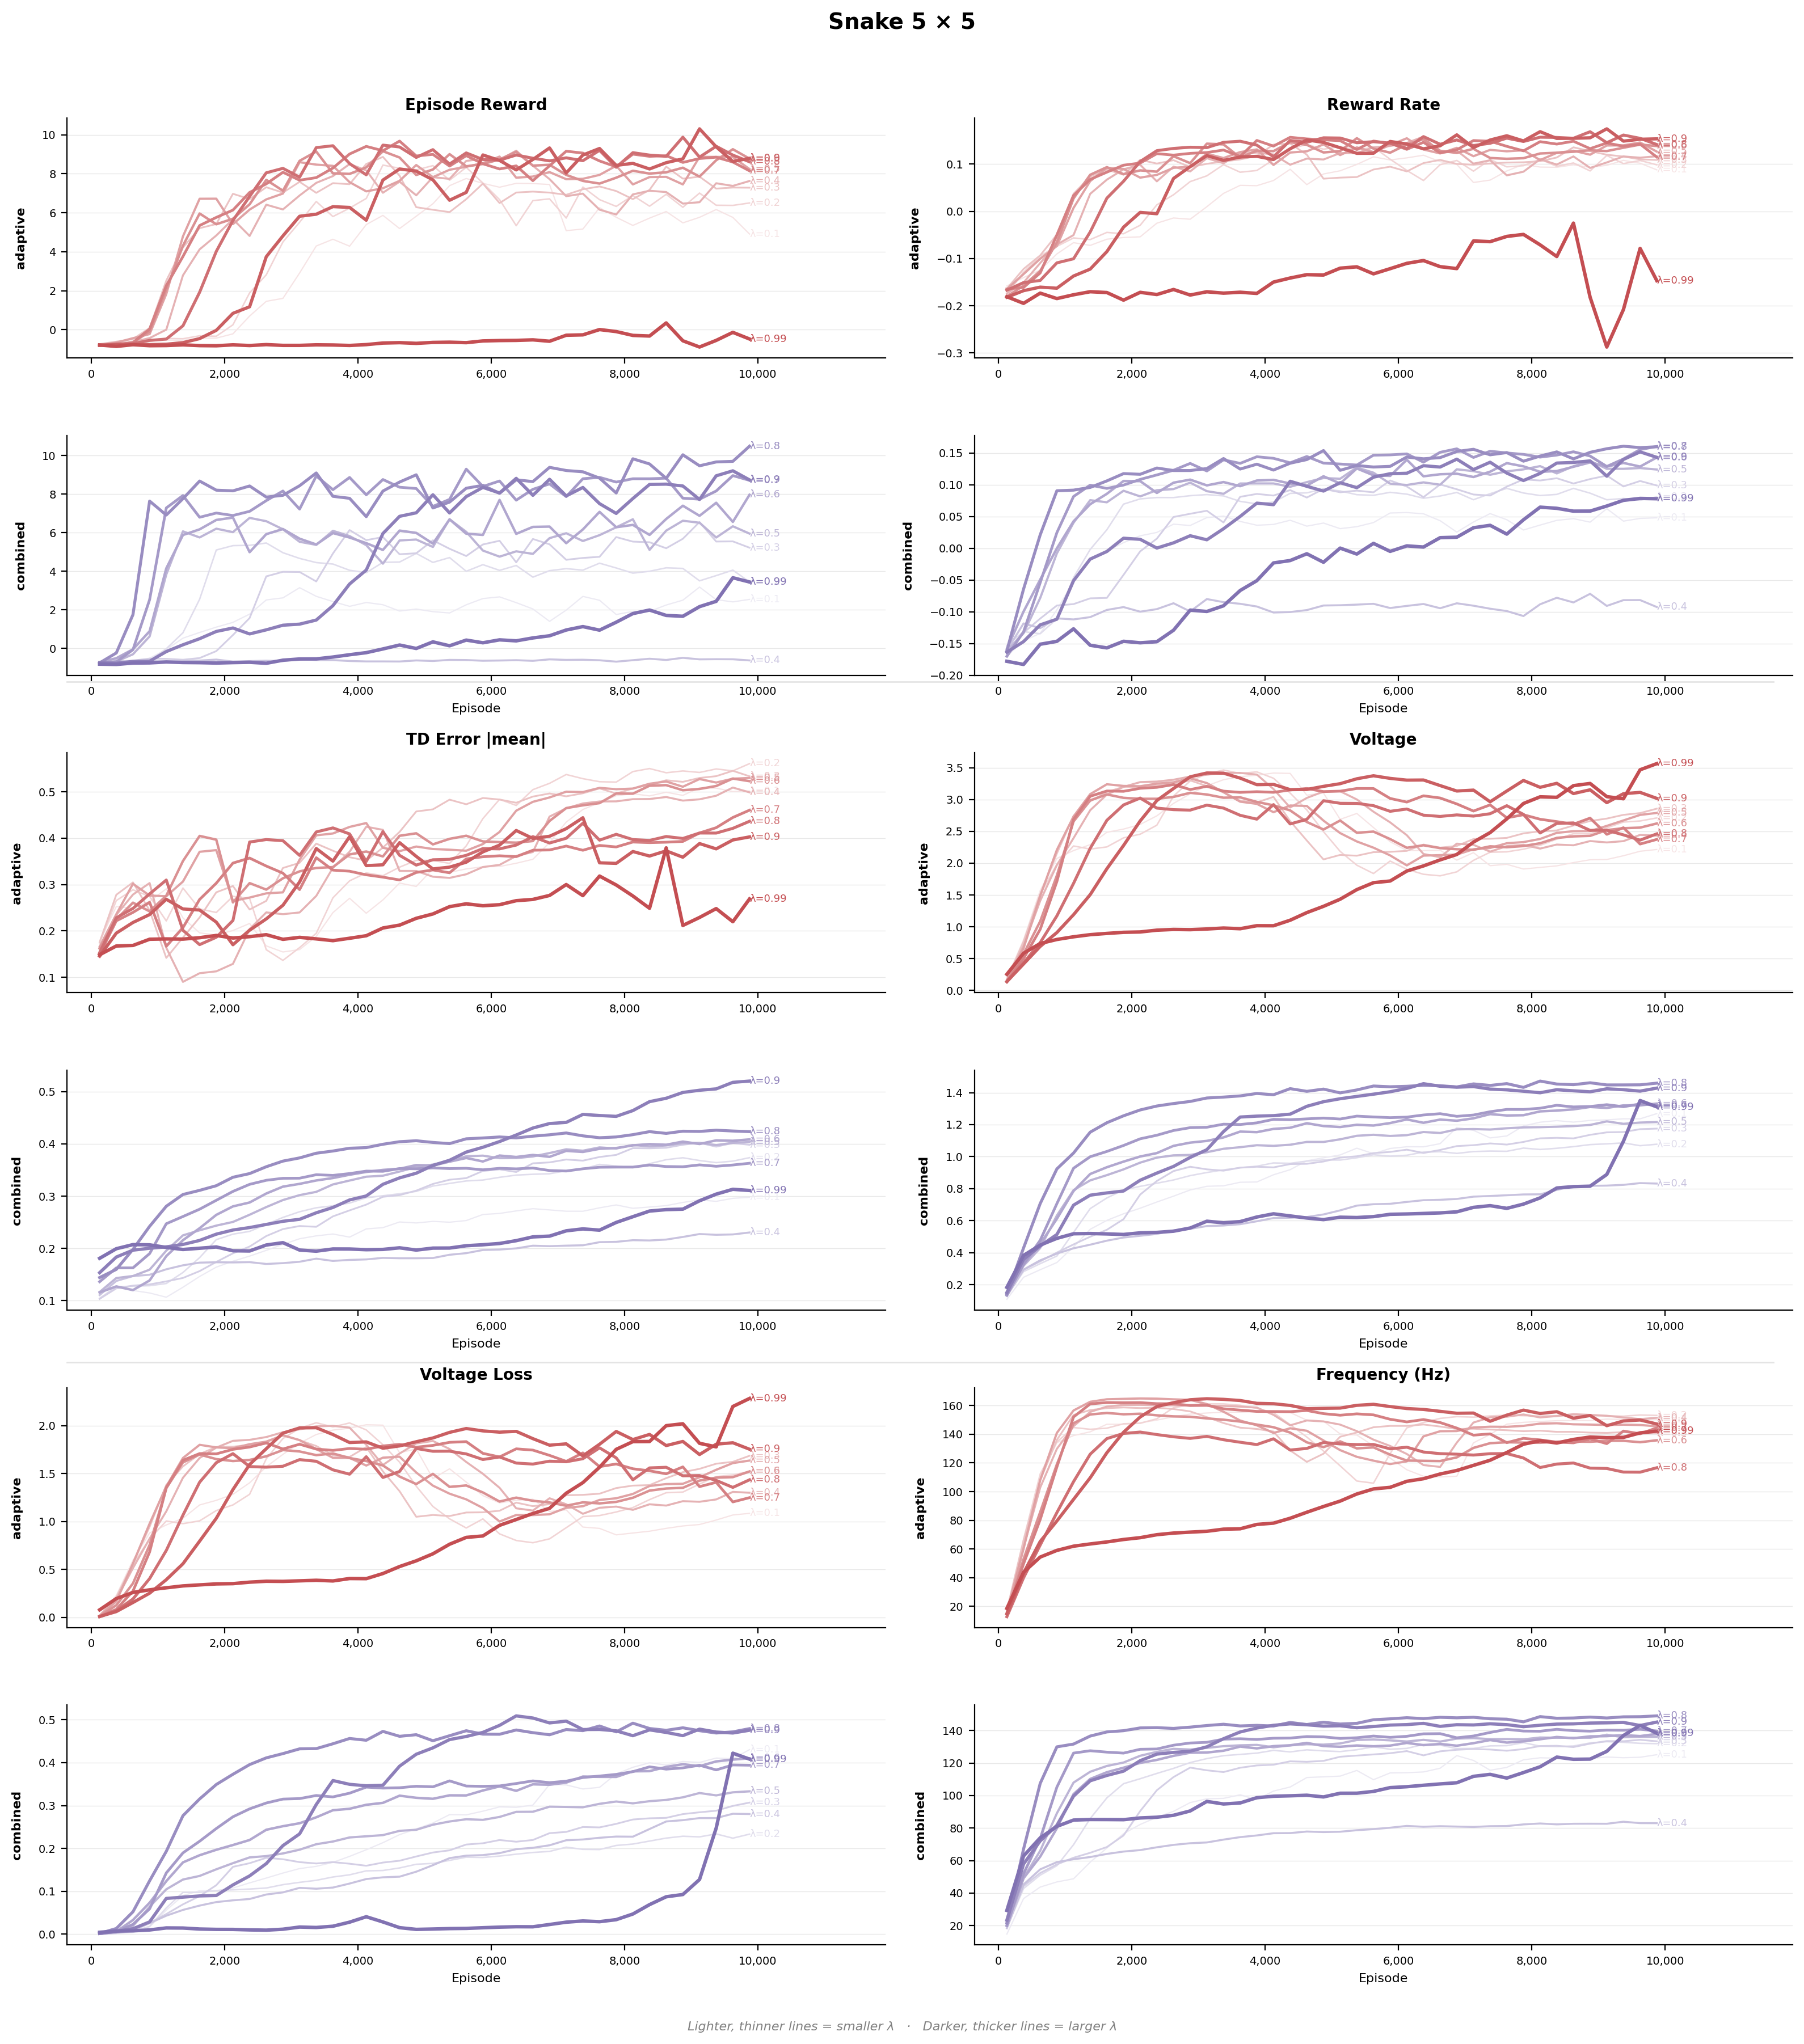
\includegraphics[width=\textwidth]{images/SnakeLambdaComparison.png}
    \caption[Lambda sweep on Snake $5\times5$]{Training performance across
    10,000 episodes on the Snake $5\times5$ task for adaptive e-prop (red)
    and the hybrid \emph{combined} variant (purple), across varying
    decay factors $\lambda \in \{0.1, 0.2, \ldots,
    0.9, 0.99\}$ (lighter, thinner lines correspond to smaller $\lambda$;
    darker, thicker lines to larger $\lambda$). Metrics reported include
    episode reward, reward rate, TD error (mean), voltage, voltage loss,
    and frequency (Hz).}
    \label{fig:snake_lambda}
\end{figure}

The distributed-family variant used for this sweep is \emph{combined}
instead of \emph{weight dist} or \emph{weight dist prop}. This
choice follows directly from the initial comparison in
Figure~\ref{fig:snake_comparison}, where \emph{combined} was
the strongest performer on Snake $5\times5$, reaching a high episode reward
faster than any other variant. Because we believe its update is dominated by the
synaptic perturbation term of \emph{weight dist} with the adaptively
routed feedback acting as a secondary contribution, we expect
\emph{combined} to behave similarly to \emph{weight dist} with respect
to $\lambda$, while benefiting from the additional stability that made it
the best-performing configuration in the initial experiment. We therefore
treat it here as a reasonable, and arguably more favorable, stand-in for
the perturbation-based family in this comparison.

On Snake, adaptive e-prop is remarkably robust to the choice of $\lambda$:
every value tested except $\lambda = 0.99$ converges to a comparable
episode reward in the range of 8 to 10, with only the speed of convergence
differing across the sweep, smaller $\lambda$ values take visibly longer to
rise but reach essentially the same plateau as the rest. Only the most
extreme value, $\lambda = 0.99$, fails to learn at all, remaining at a
slightly negative episode reward for the full $10,000$ episodes and showing
the same large, erratic swings in reward rate, voltage, and voltage loss
that elsewhere in this chapter have accompanied a destabilized critic. The
\emph{combined} variant is comparatively less uniform: most values of
$\lambda$ between 0.5 and 0.9 reach a similar high reward, but
$\lambda = 0.4$ fails to learn within the training budget, and
$\lambda = 0.99$ learns somewhat but only after a long initial period
of flat reward. The failure of $\lambda = 0.4$ is
worth treating with particular caution, since it sits in the middle of a
range that otherwise learns reliably, with $0.3$, $0.5$, and $0.6$ all
reaching the high-reward plateau on either side of it. Because each point
in this sweep is a single run, as noted
above, this is more plausibly read as an unlucky individual run, for
instance an unfavorable initialization or an early run of bad exploration
that the perturbation-based update never fully recovered from, than as
evidence that $\lambda = 0.4$ is itself a uniquely poor choice for
\emph{combined}. Stochastic learning rules of this kind can occasionally
fail to get off the ground even at a hyperparameter setting that is
otherwise unremarkable, and without repeated seeds at this specific value
we cannot distinguish that explanation from a genuine, reproducible
sensitivity to $\lambda = 0.4$.

As we will see in Section~\ref{sec:lambda_comparison}, this is the
opposite of the ordering observed on the Pac-Man randomized layouts
problem, where it is the distributed-style variant that tolerates a wide
range of $\lambda$ while adaptive e-prop shows an inconsistent and often
delayed learning onset. Here, on Snake, it is adaptive e-prop that appears
to be the more forgiving of the two with respect to $\lambda$, with only
the single extreme value $\lambda = 0.99$ causing outright failure, while
\emph{combined} shows a less monotonic and somewhat narrower band of
$\lambda$ values for which it learns promptly. Taken together, the two
experiments will support the broader argument of this chapter: 
neither structured feedback-based credit assignment nor
perturbation-based credit assignment is uniformly more robust to the
decay factor $\lambda$. Which rule tolerates a wider or more reliable
range of $\lambda$ appears to depend on the task, and possibly on other
interacting factors such as architecture depth or reward sparsity that
differ between Snake and Pac-Man, and not an intrinsic property
of either algorithm.

\subsection{Depth Comparison}
\label{subsec:snake-depth-comparison}

\begin{figure}[htpb]
    \centering
    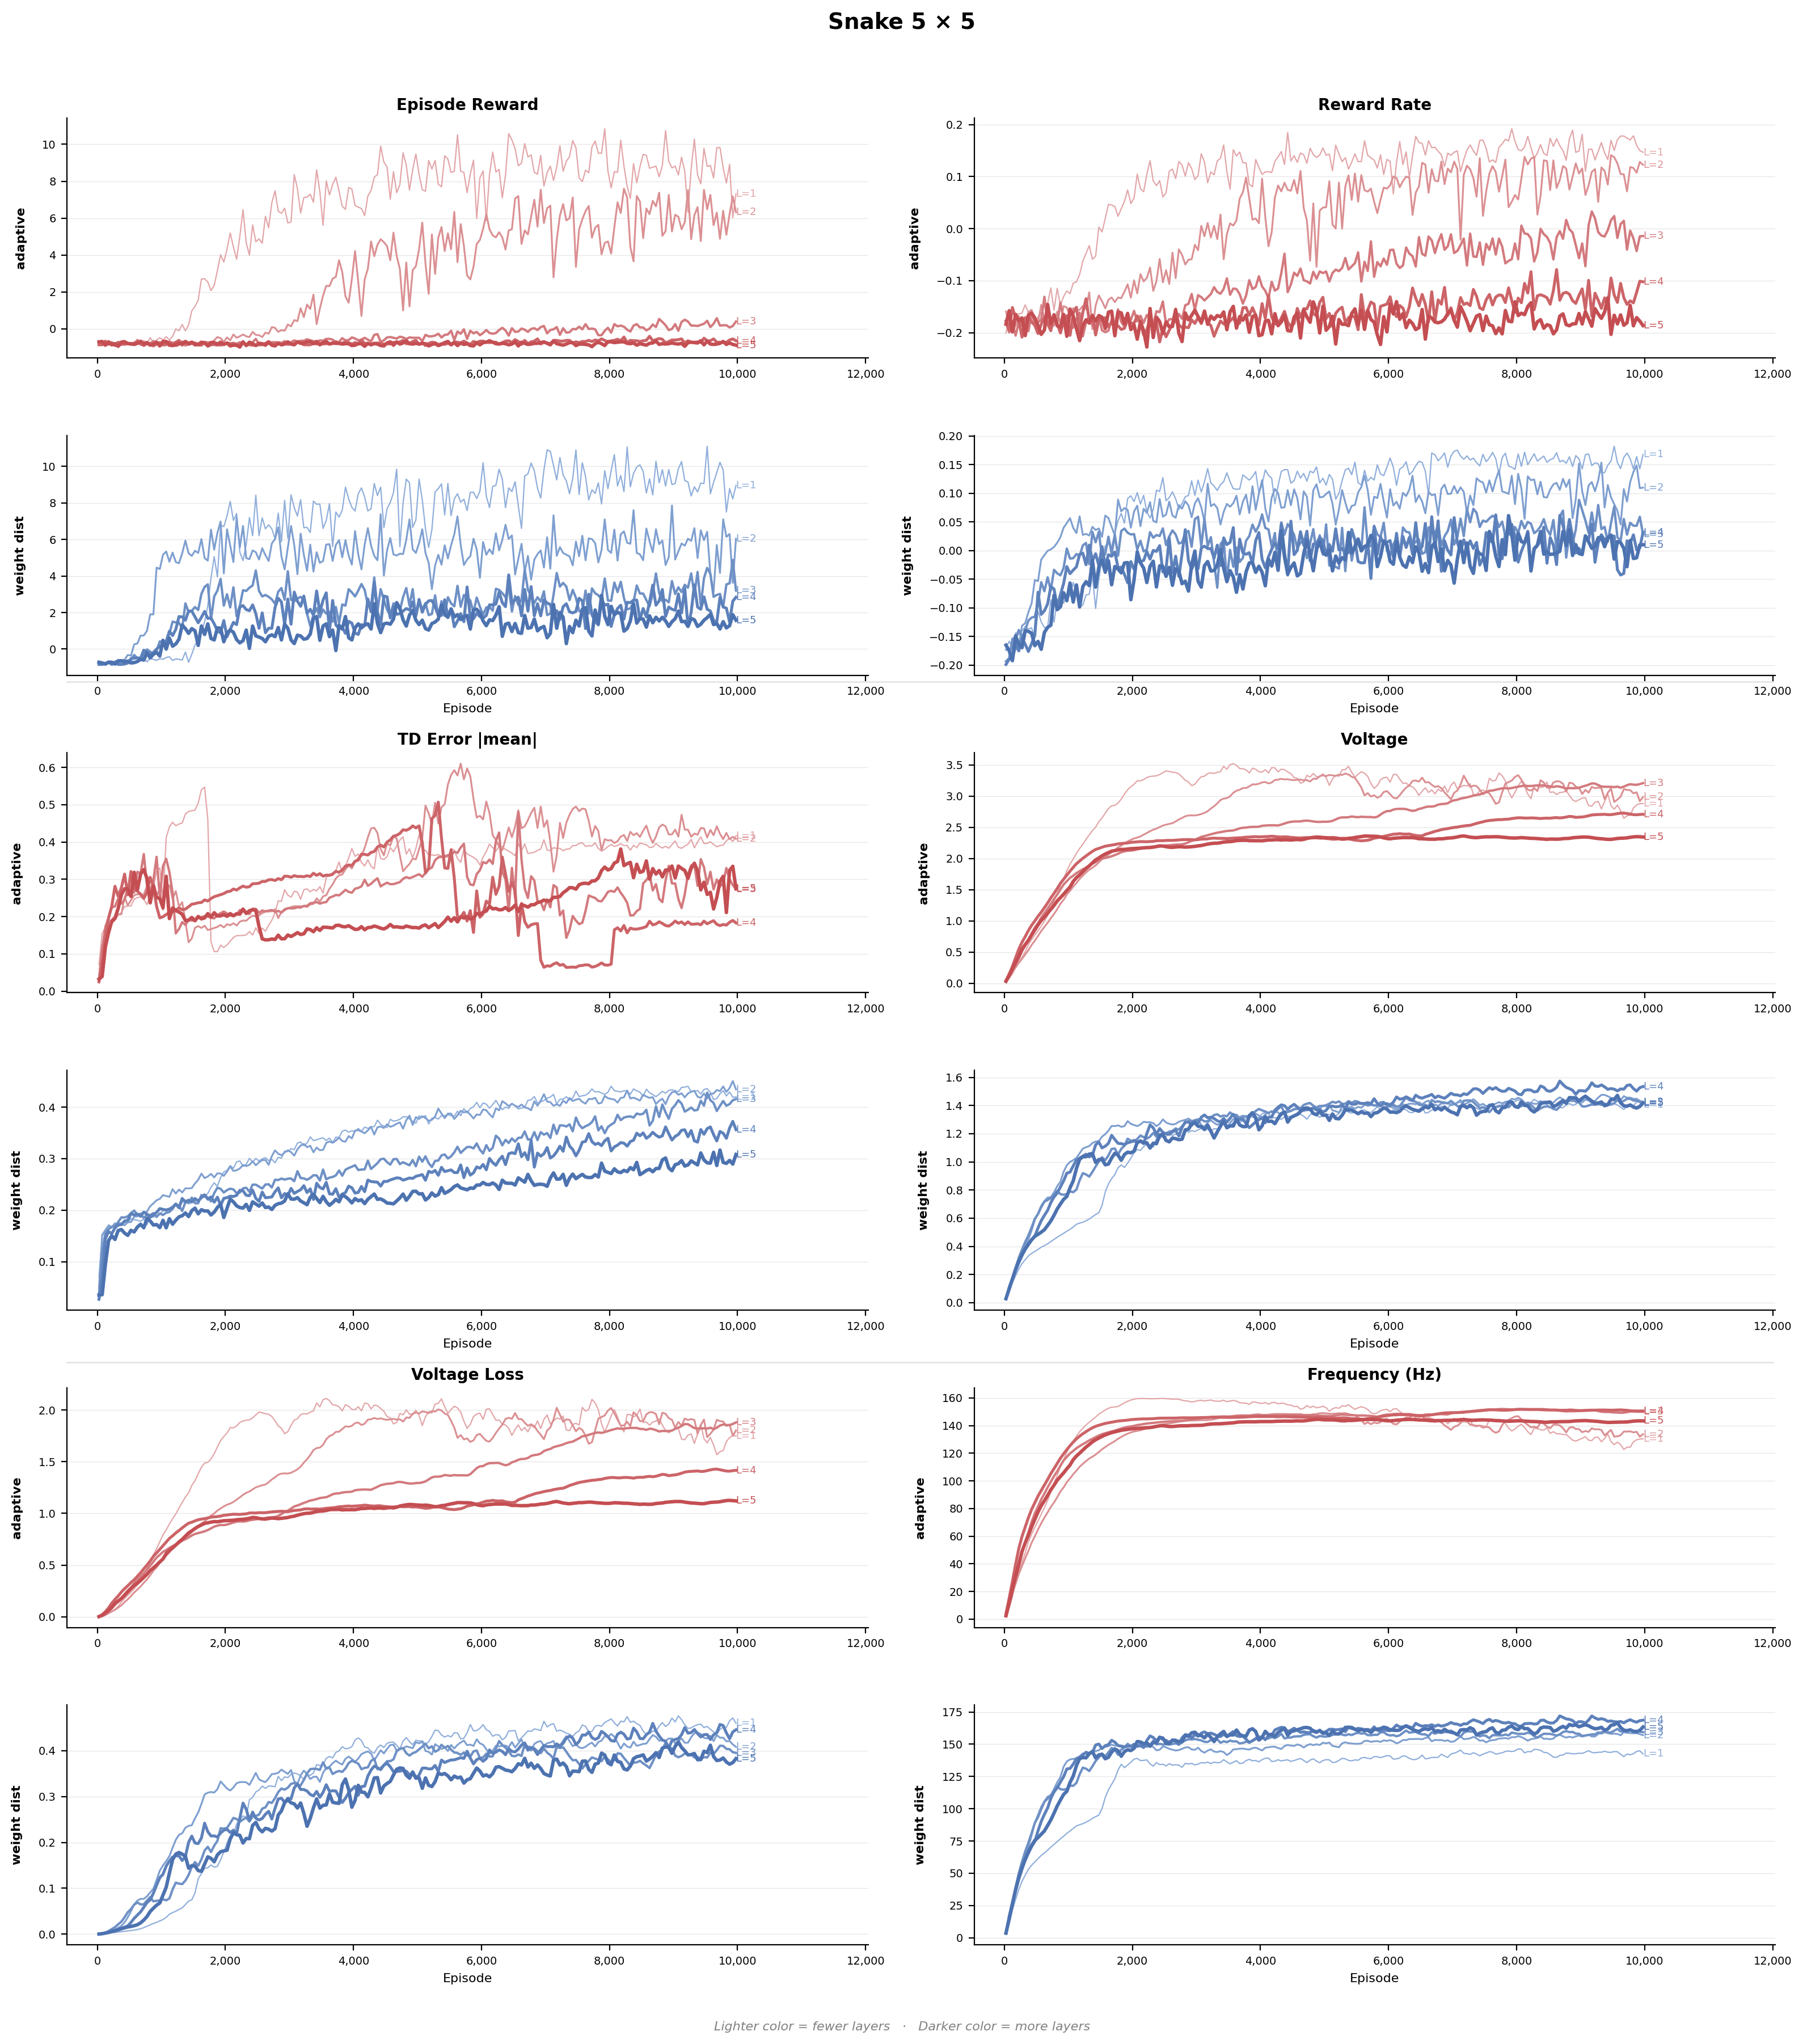
\includegraphics[width=1.0\linewidth]{images/SnakeLayersComparison.png}
    \caption[Effect of network depth on Snake $5\times5$]{Effect of network depth on the Snake $5\times5$ task, comparing adaptive e-prop
    (red, upper sub-row of each metric) and distributed e-prop (\emph{weight dist}, blue, lower
    sub-row) across networks with different numbers of layers. Colour shade encodes depth: lighter
    shades correspond to shallower networks and darker shades to deeper ones. Each panel reports
    one of the six standard metrics (episode reward, reward rate, mean absolute TD error, voltage,
    voltage loss, and frequency in Hz) over $10{,}000$ episodes. Increasing depth lengthens the
    causal path between input and output, and the figure shows how the learning of each rule
    degrades as that path grows.}
    \label{fig:snake-depth-comparison}
\end{figure}

Figure~\ref{fig:snake-depth-comparison} reports the six standard metrics for both rules across
networks of increasing depth, with lighter shades denoting shallower networks and darker shades
deeper ones. In
the episode reward and reward rate panels, both rules display a clear ordering by depth where the
shallowest networks reach the highest reward and reward rate, and the curves fall steadily as
layers are added. The rules differ in how pronounced this decline is. For adaptive e-prop the
spread across depths is wide: the shallowest network reaches a reward of roughly eight to ten,
while the deepest networks stay close to zero for the full $10{,}000$ episodes. For distributed
e-prop the spread is narrower: the shallowest network reaches a comparable reward, and although
the deeper networks again score lower, every depth tested converges to a clearly positive
reward. The reward rate panels follow the same pattern, with the deepest adaptive networks
settling at negative values and the deepest distributed networks remaining near zero or above.

The remaining panels describe the value-error and spiking dynamics. In the TD error panels,
both rules show an error that grows over training and increases with depth, with the adaptive
curves visibly noisier and reaching larger values while the distributed curves grow more
smoothly. The voltage and voltage-loss panels show a consistent gap between the rules, we have that adaptive
e-prop reaches a higher membrane voltage, around three, and a higher voltage loss, both rising
with depth, whereas distributed e-prop holds a lower and flatter voltage, around one and a half,
together with a small voltage loss across all depths. The firing frequency converges to a
similar high band of roughly $140$ to $170$ Hz for both rules at every depth, separating the
configurations only marginally.

The depth comparison above invites a tempting but, we believe, mistaken conclusion: that
distributed e-prop is intrinsically better suited to longer causal paths. Because we knew from the
outset that e-prop with aligned feedback can be slow to start, learning only once its feedback
pathway and internal dynamics have settled into agreement, we ran a deeper configuration for a
much longer horizon to test this directly. We do so under two update schemes for a five-layer
network on Snake $5\times5$: Figure~\ref{fig:snake-extended-perstep} applies the weight update
continuously, once per environment step, while Figure~\ref{fig:snake-extended-perepisode} applies
it once per episode. Both span roughly $100{,}000$ episodes.

The extended runs reverse the impression left by the fixed-budget comparison, and they do so under
both update schemes. The distributed variants behave exactly as before: they reach a usable reward
within the first few thousand episodes and then stop improving, holding that plateau for the rest
of training, whether the weight update is applied continuously (Figure~\ref{fig:snake-extended-perstep})
or once per episode, where the \emph{combined} variant behaves much like \emph{weight dist}
(Figure~\ref{fig:snake-extended-perepisode}). Adaptive e-prop, by contrast, spends a long initial
phase near zero reward, the signature of feedback alignment that has not yet taken effect, and only
then begins to learn. Once it does, it continues to improve past the level at which the distributed
variants stalled, and is still improving when each run ends. The spiking-dynamics panels tell the
same story in both figures: adaptive e-prop operates at a markedly higher membrane voltage and
voltage loss, rising during its learning phase, while the distributed variants stay low and flat,
and the firing frequencies remain in a similar high band with adaptive e-prop running slightly lower.

We read this as a caution, and even then only provisionally. The
deep-network collapse of adaptive e-prop in the depth comparison is not evidence that the rule
cannot handle longer causal paths; in this case, it appears to be an artifact of the training
budget, since the same configuration begins to learn the task when given more time. What seems
to distinguish the two rules here is less their capability than their dynamics: distributed
e-prop tends to find a reasonable solution quickly and then improve little further, while
adaptive e-prop is slow to start, plausibly because feedback alignment takes time, without
showing clear signs of being fundamentally limited by depth. These remain possibilities, 
because the hyperparameters have not been tuned exhaustively, and a given
setting can favor one rule while handicapping the other, any apparent advantage may reflect the
particular configuration tested rather than a property of the algorithm itself. We therefore do
not claim that either rule is better at handling causal path length, and present this longer run
only as an example of why the immediate interpretation of the depth comparison cannot be taken
at face value.

\begin{figure}[H]
    \centering
    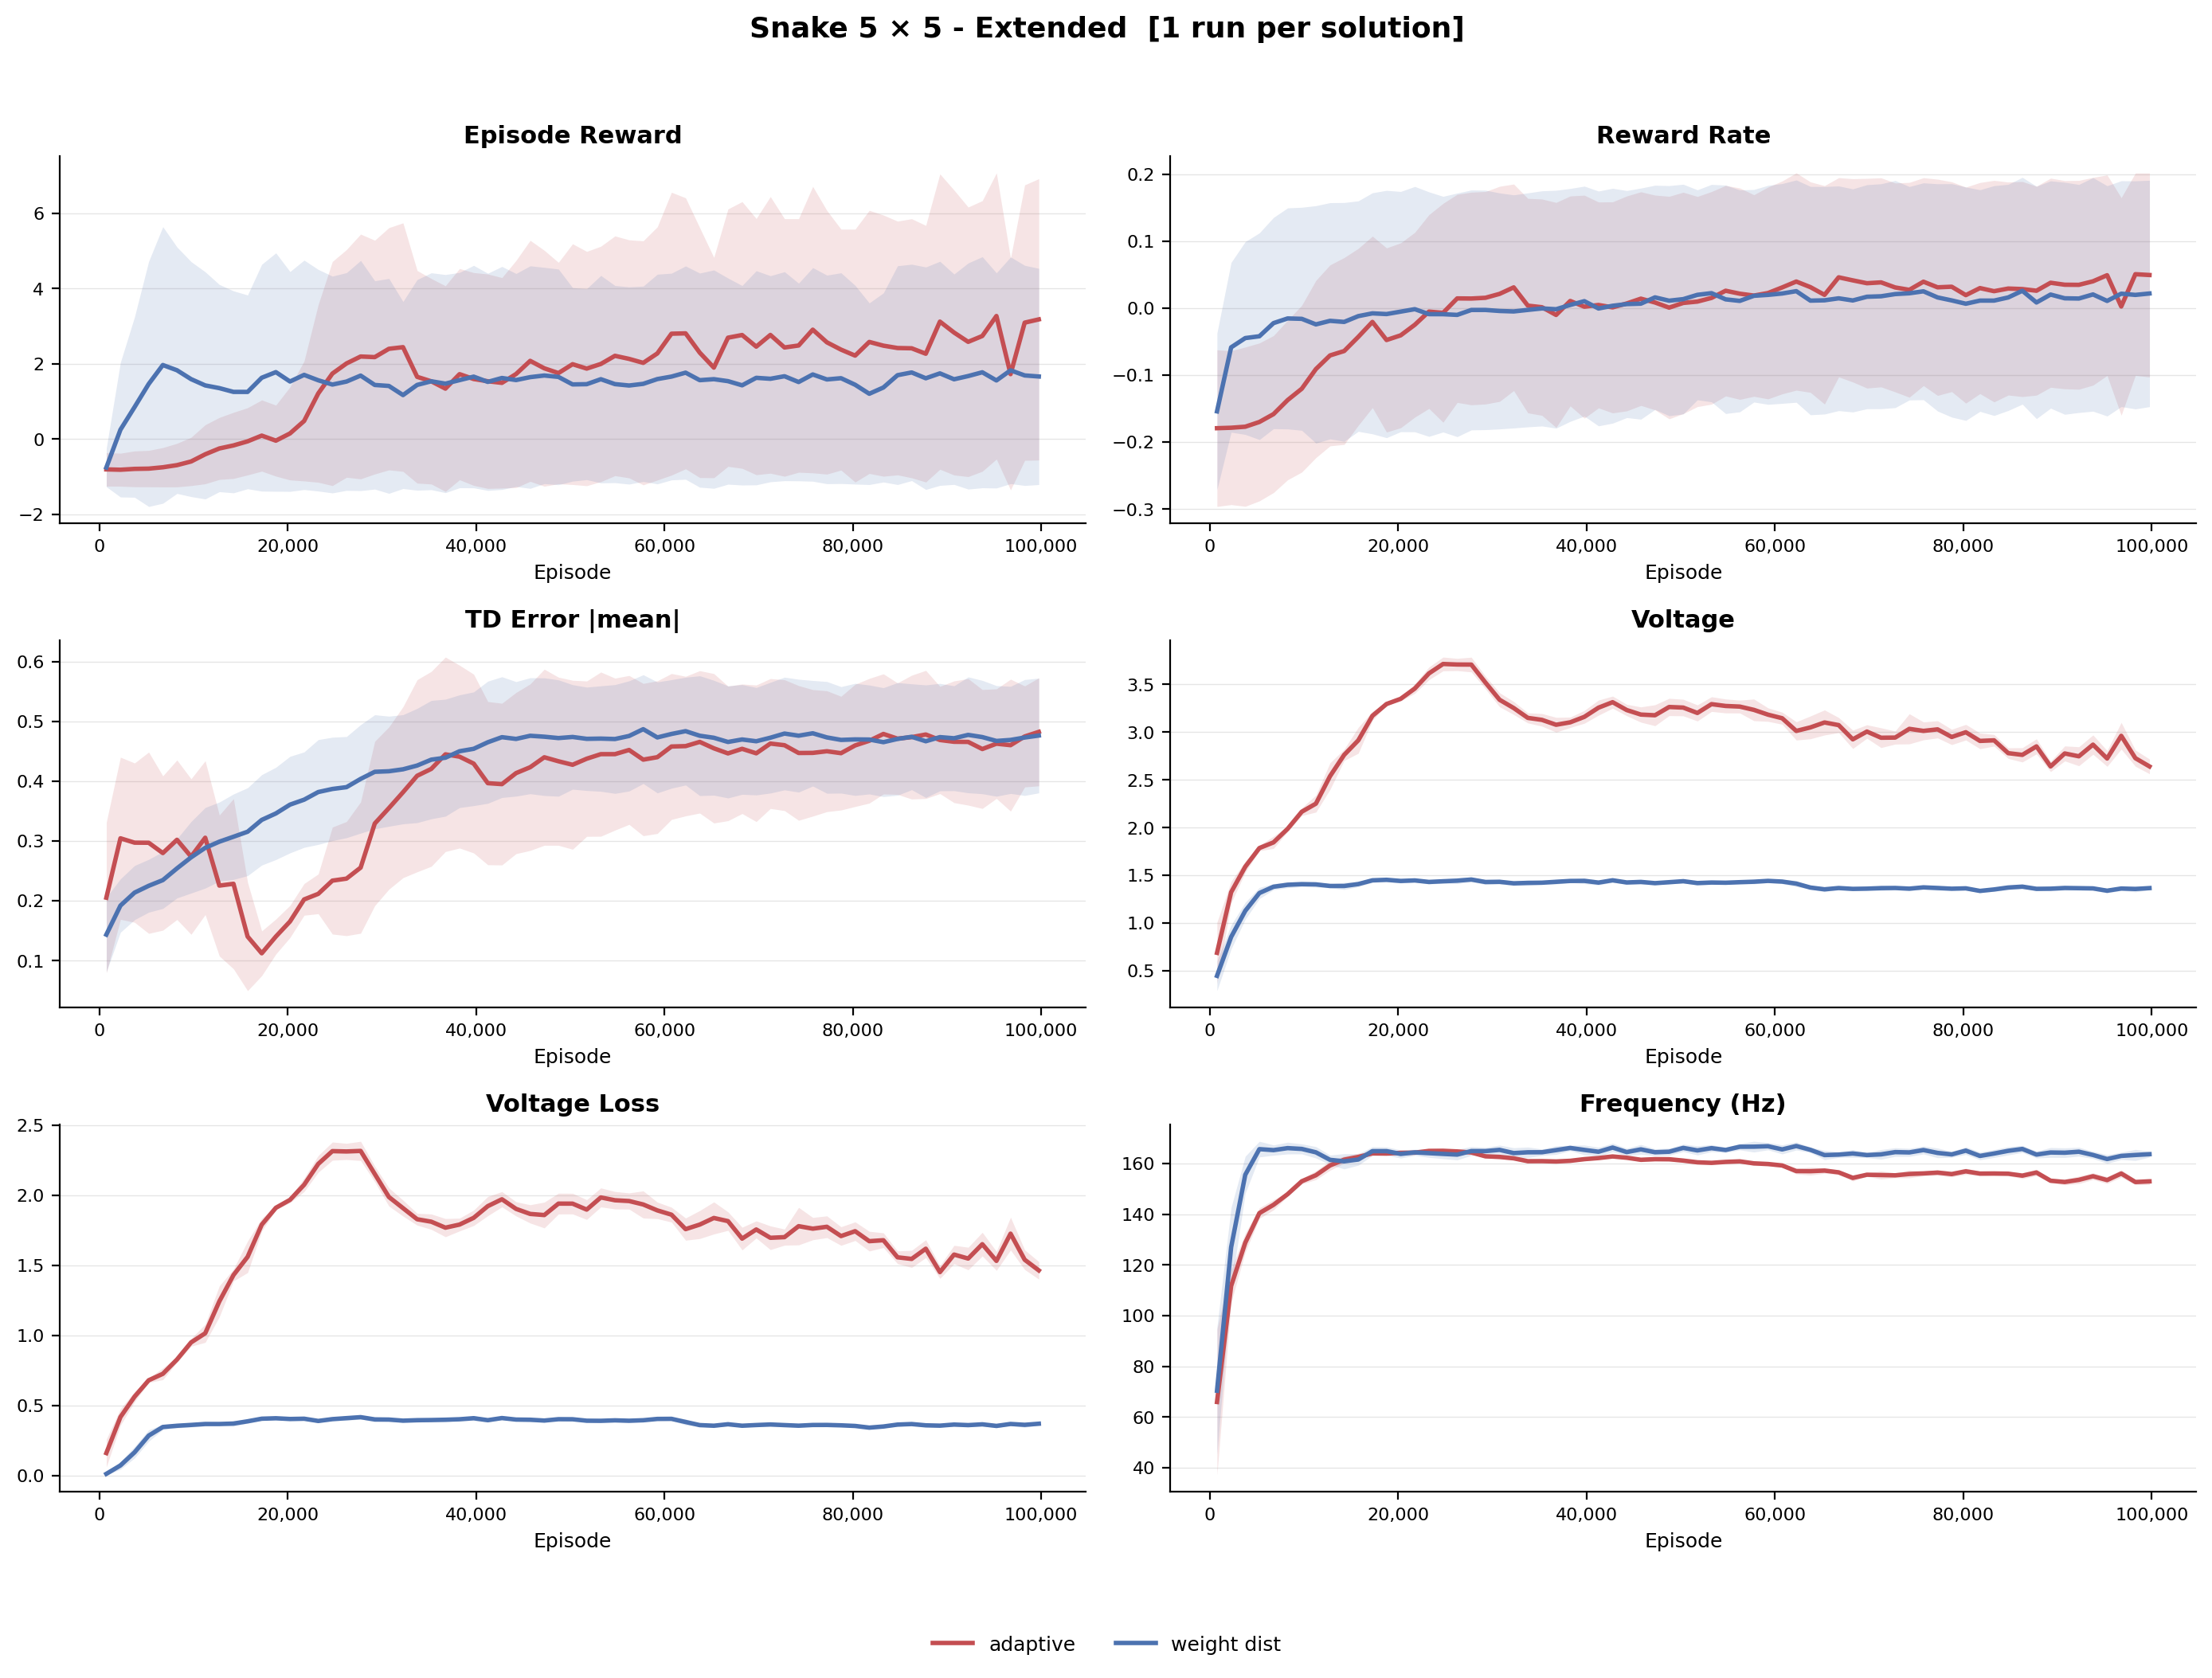
\includegraphics[width=1\linewidth]{images/comparison_extended_1_runs.png}
    \caption[Extended training, 5-layer network, updates per step (Snake)]{Extended,
    longer-horizon training on Snake $5\times5$ with a five-layer network, comparing adaptive
    e-prop (red) with distributed e-prop (\emph{weight dist}, blue) when the weight update is
    applied continuously, once per environment step. One run per configuration; the six standard
    metrics are shown over roughly $100{,}000$ episodes. Distributed e-prop converges within the
    first few thousand episodes and then holds a plateau, whereas adaptive e-prop makes little
    progress for an extended initial period before beginning to learn and overtaking it.}
    \label{fig:snake-extended-perstep}
\end{figure}

Comparing the two update schemes is itself informative. The per-episode updates were clearly
beneficial for both rules, adaptive e-prop and \emph{weight dist} each reach a higher episode
reward and reward rate under per-episode updating (Figure~\ref{fig:snake-extended-perepisode})
than under the continuous, per-step scheme (Figure~\ref{fig:snake-extended-perstep}). The
\emph{combined} variant, by contrast, was consistently the weakest of the three across the
performance metrics. This is genuinely surprising, since in the single-layer comparison of all
rules on this same task (Figure~\ref{fig:snake_comparison}) combined e-prop was among the
better-performing variants; the deeper, longer-horizon setting evidently reverses that standing.

\begin{figure}[H]
    \centering
    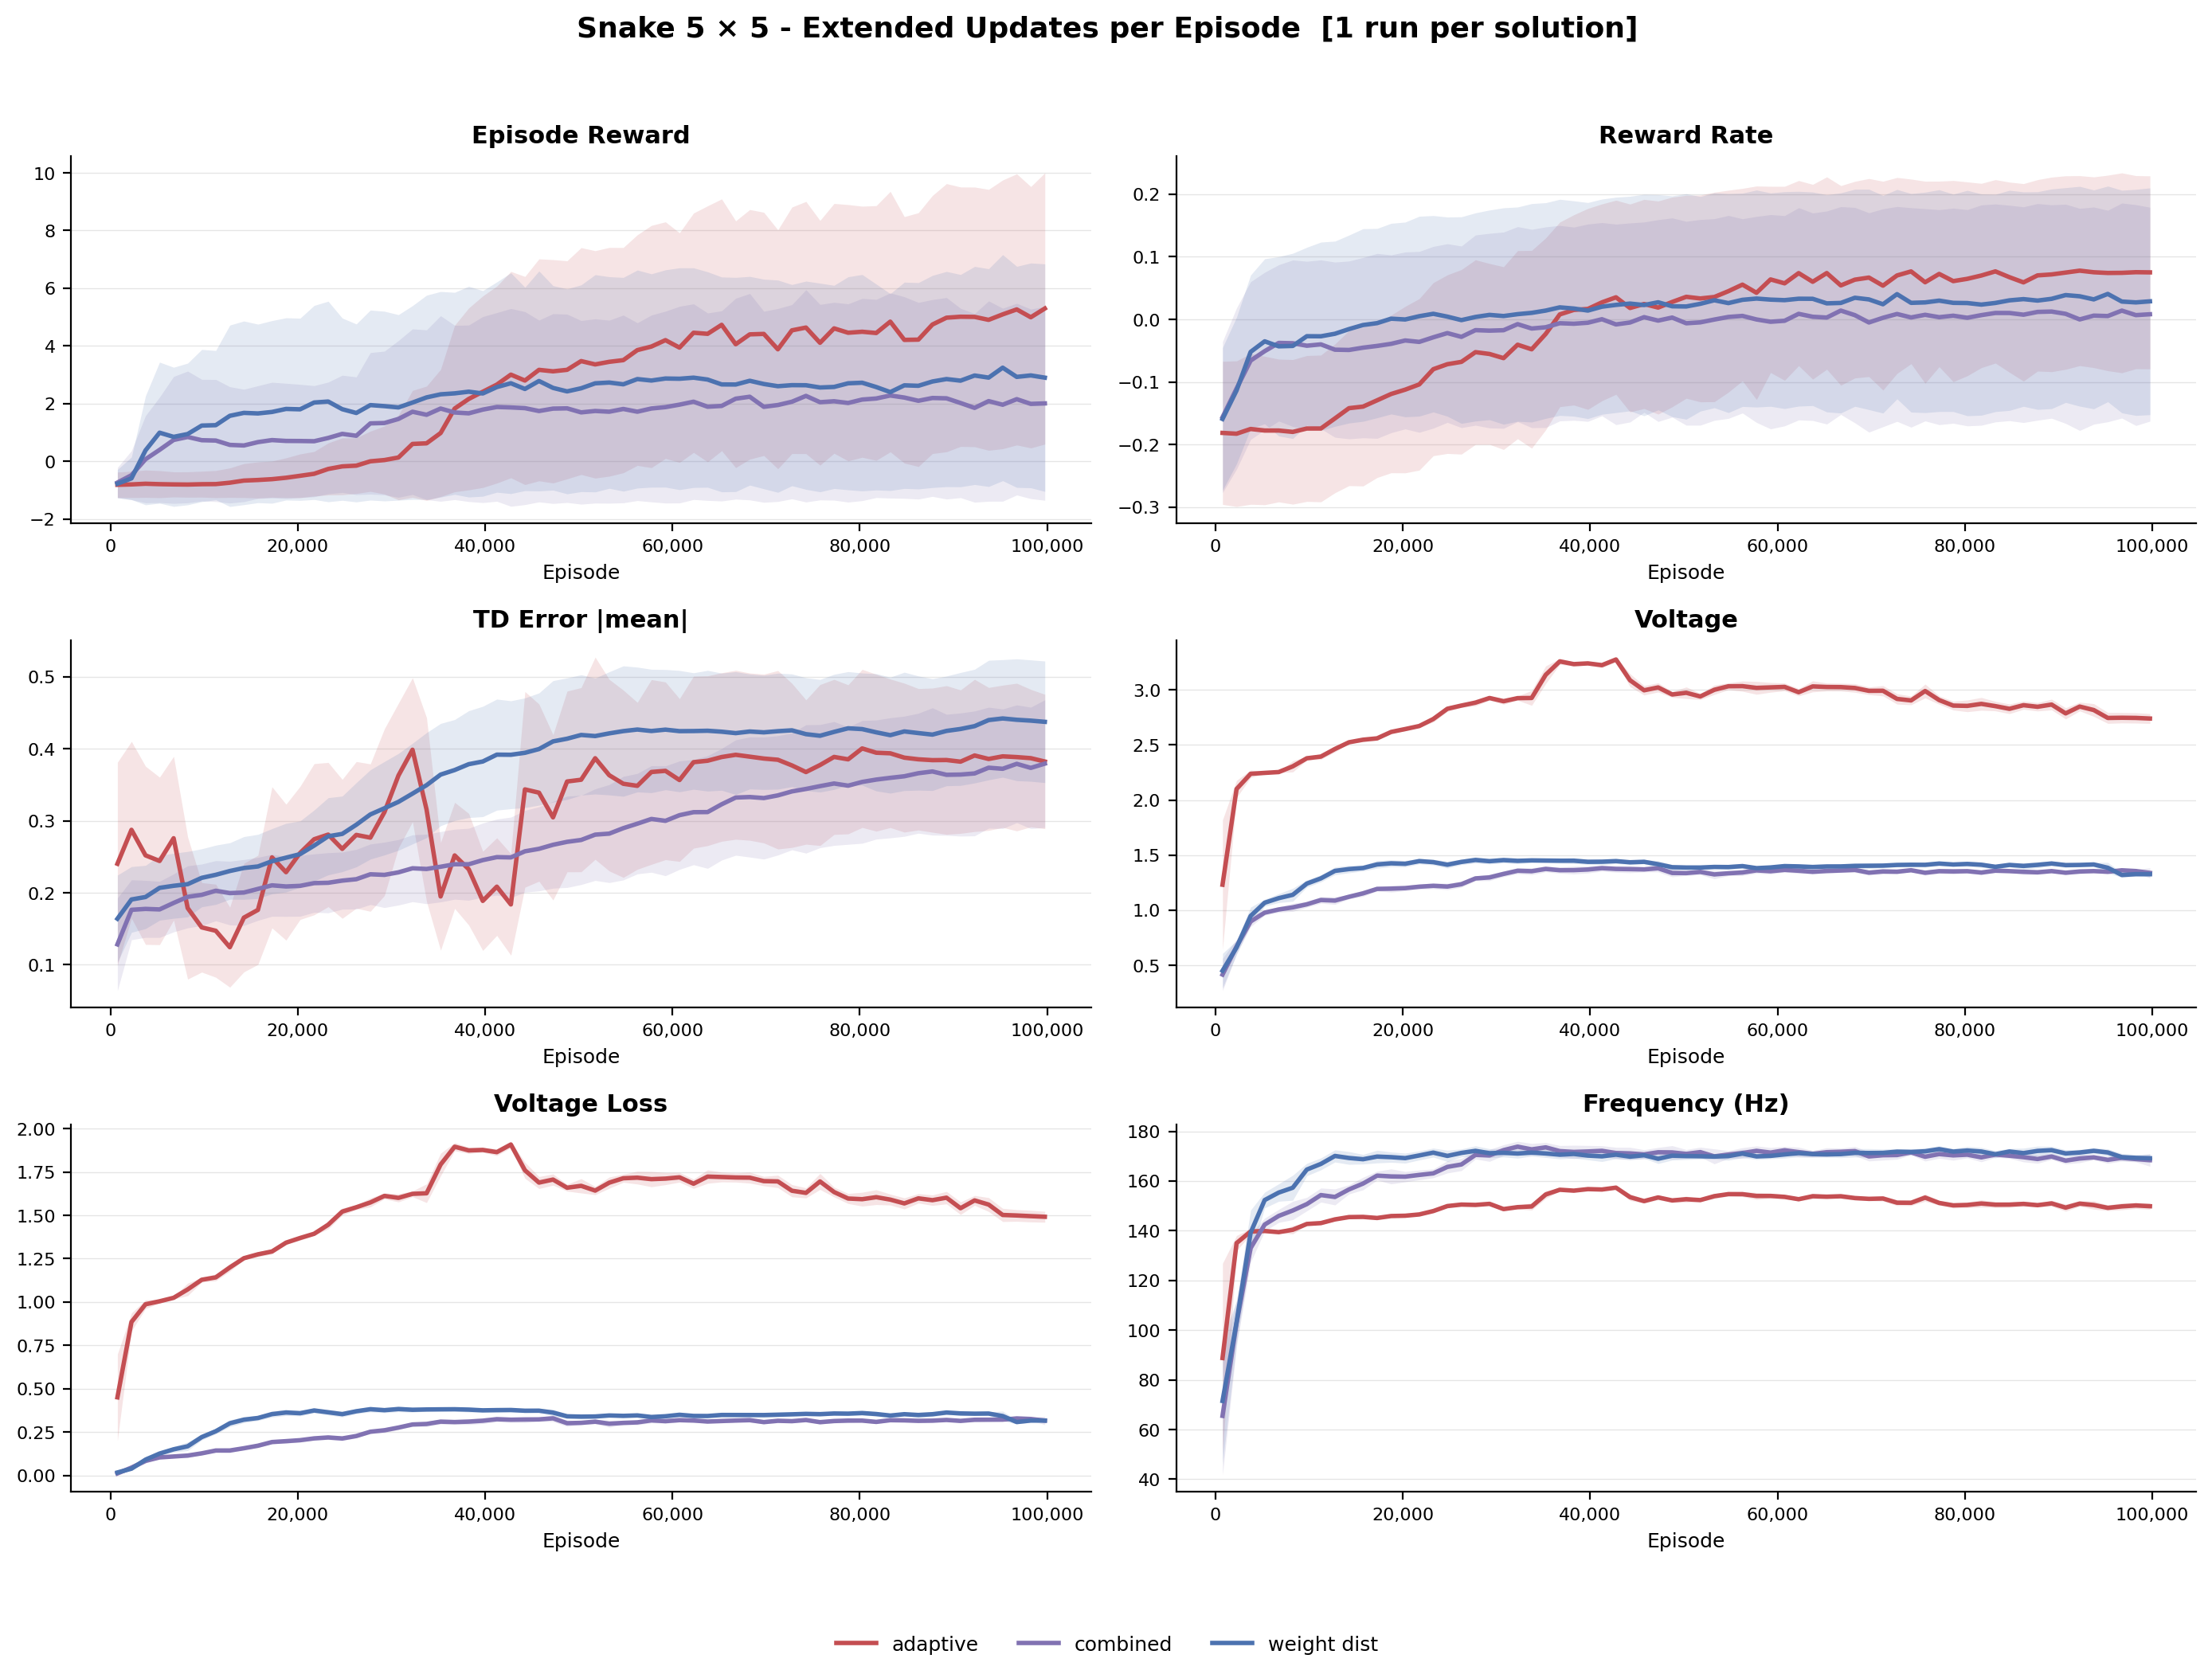
\includegraphics[width=1\linewidth]{images/comparison_extended_updates_per_episode_1_runs.png}
    \caption[Extended training, 5-layer network, updates per episode (Snake)]{The same extended
    setup as Figure~\ref{fig:snake-extended-perstep}, but with the weight update applied once per
    episode. Adaptive e-prop (red) is compared with two distributed
    variants, \emph{weight dist} (blue) and \emph{combined} (purple). One run per configuration;
    the six standard metrics over roughly $100{,}000$ episodes. The qualitative pattern is
    unchanged: the distributed variants plateau early while adaptive e-prop starts slowly and then
    continues to improve past them.}
    \label{fig:snake-extended-perepisode}
\end{figure}

Figure~\ref{fig:snake-qualitative-depth} provides a qualitative look inside
a single representative episode for \emph{weight dist} at two different
network depths. The 2-layer network produces a value estimate with clear
predictive structure, rising ahead of reward events and falling ahead of
penalties, while the 5-layer network develops a comparatively flat and
unstructured estimate that fails to anticipate upcoming events. The action
probability show a possible failure reason, the shallower network retains
a more distributed policy with intermediate probability mass across multiple
actions, whereas the deeper network collapses to a near-deterministic policy
at almost every timestep, which limits exploration and therefore learning. 
Both observations are consistent with the
performance plateau seen in Figures
~\ref{fig:snake-extended-perstep}, ~\ref{fig:snake-extended-perepisode} and ~\ref{fig:snake-depth-comparison}, though whether
the observations are a cause or a consequence 
is difficult to establish from these results alone.

\begin{figure}[H]
    \centering
    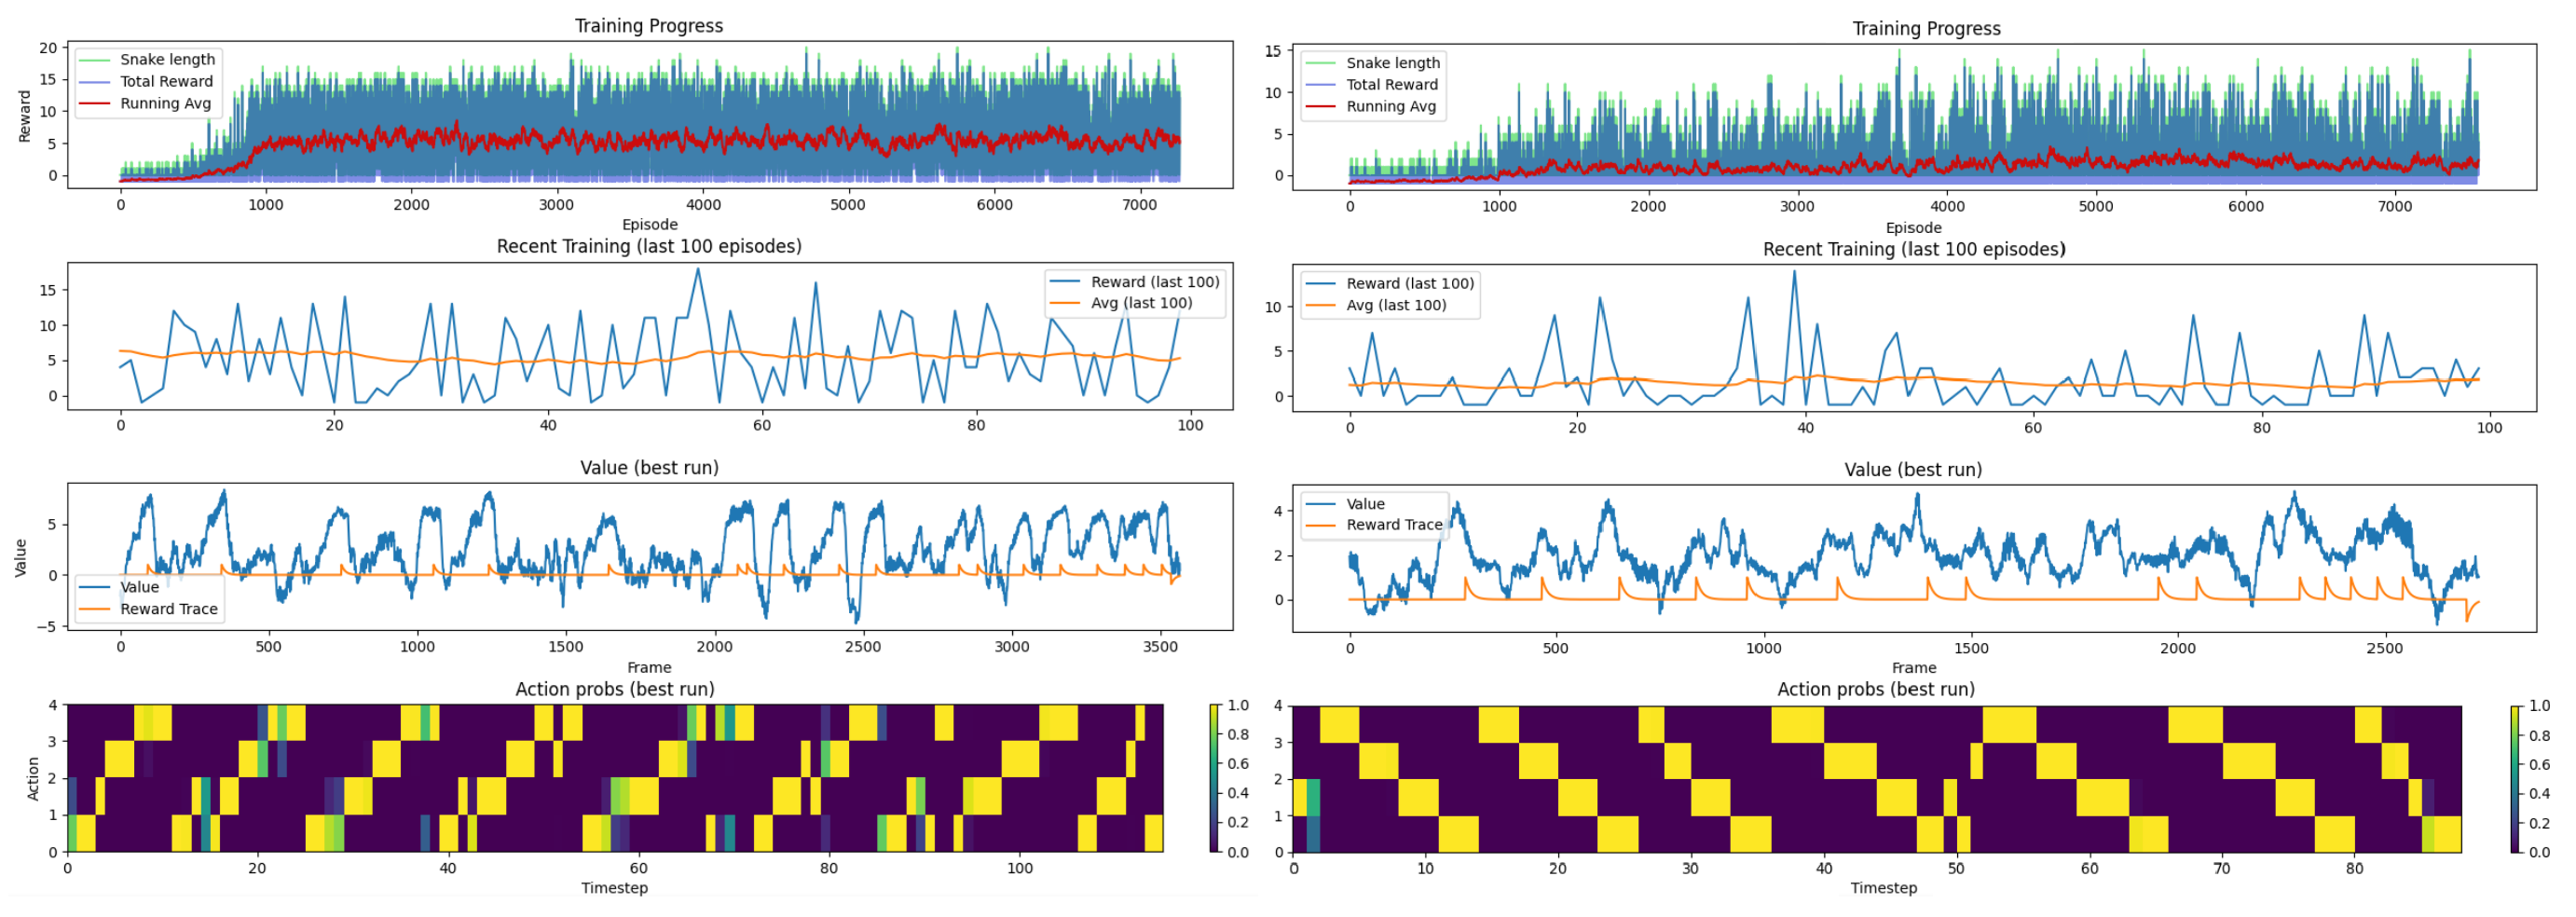
\includegraphics[width=1\linewidth]{images/SnakeQualitative2vs5Layers.png}
    \caption[Qualitative \emph{weight dist}, depth comparison]{Qualitative comparison of \emph{weight dist} on Snake
    $5 \times 5$ at two network depths. Each column shows a representative
    episode from a 2-layer (left) and 5-layer (right) network at a similar
    stage of training. From top to bottom: training progress over all episodes;
    reward over the most recent 100 episodes against its running mean; the value
    estimate $V_t$ against the reward trace; and a heatmap of the action
    probabilities through the episode.}
    \label{fig:snake-qualitative-depth}
\end{figure}

\subsection{Reward-based regularization Exploration}
\label{sec:regularization-exploration}

Figure~\ref{fig:snake-regularization} explores the effect of the
reward-based regularization terms introduced in
Section~\ref{subsec:regularization} on the \emph{weight dist}
variant on Snake $5 \times 5$, sweeping over the regularization strength
$c_{reg}$. Two broad trends are visible across the metrics. First,
increasing regularization strength consistently reduces task performance,
suggesting that beyond a certain point the regularization signal competes
with the task reward signal for control of the perturbation traces, pulling
weight updates away from task-relevant directions. Second, the two
regularization targets, voltage and firing frequency, respond differently
to the same regularization pressure.

Voltage regularization appears to be the easier objective for the network
to satisfy: the voltage metrics respond clearly and consistently to
increasing $c_{reg}$, with membrane potentials brought closer to a
well-regulated range even at moderate regularization strengths. A plausible
explanation for why this works so well in the distributed e-prop framework
is that voltage deviation is an entirely local quantity, observable at the
level of a single neuron without any reference to the global network state.
This makes it a natural fit for the perturbation-based update rule, where
each neuron acts as an independent stochastic actor: the local voltage
reward provides a local evaluative signal that is directly compatible with
the local perturbation traces, without requiring any credit to be routed
across the network. This observation opens an interesting direction for
future work, namely the design of other local reward signals that exploit
this compatibility more deliberately, potentially allowing neurons to
optimize local objectives that complement the global task reward in ways
that structured feedback rules cannot easily support.

Frequency regularization proves harder to enforce, with only a modest effect
visible even at larger values of $c_{reg}$. The reasons for this are not
entirely clear, and we do not attempt to offer a definitive explanation here.

It is worth noting that we were unable to make voltage regularization work
within the standard e-prop framework. Although the exact cause remains
unclear, a likely contributing factor is that the standard e-prop voltage
regularization update depends directly on the presynaptic spike train and
adaptive threshold, and has no mechanism to suppress itself when the membrane
is in a pathological regime. The perturbation trace, by contrast, naturally
carries little signal when the membrane is far from threshold, since the
perturbations are unlikely to have influenced the spike output in that
regime, which effectively gates the regularization update and prevents it
from generating runaway effects. The standard e-prop update lacks this
self-suppression, and may therefore produce large and poorly directed weight
changes precisely when the membrane dynamics are most unstable, reinforcing
the pathology. Whether a modified formulation that
incorporates a similar gating mechanism could recover comparable behavior
remains an open question.

Surprisingly the best performance seen until now is given by the non 
regularized run with $c_{reg}=0.0$ as it can be seen in ~\ref{tab:snake-best100-score}.

\begin{figure}[H]
    \centering
    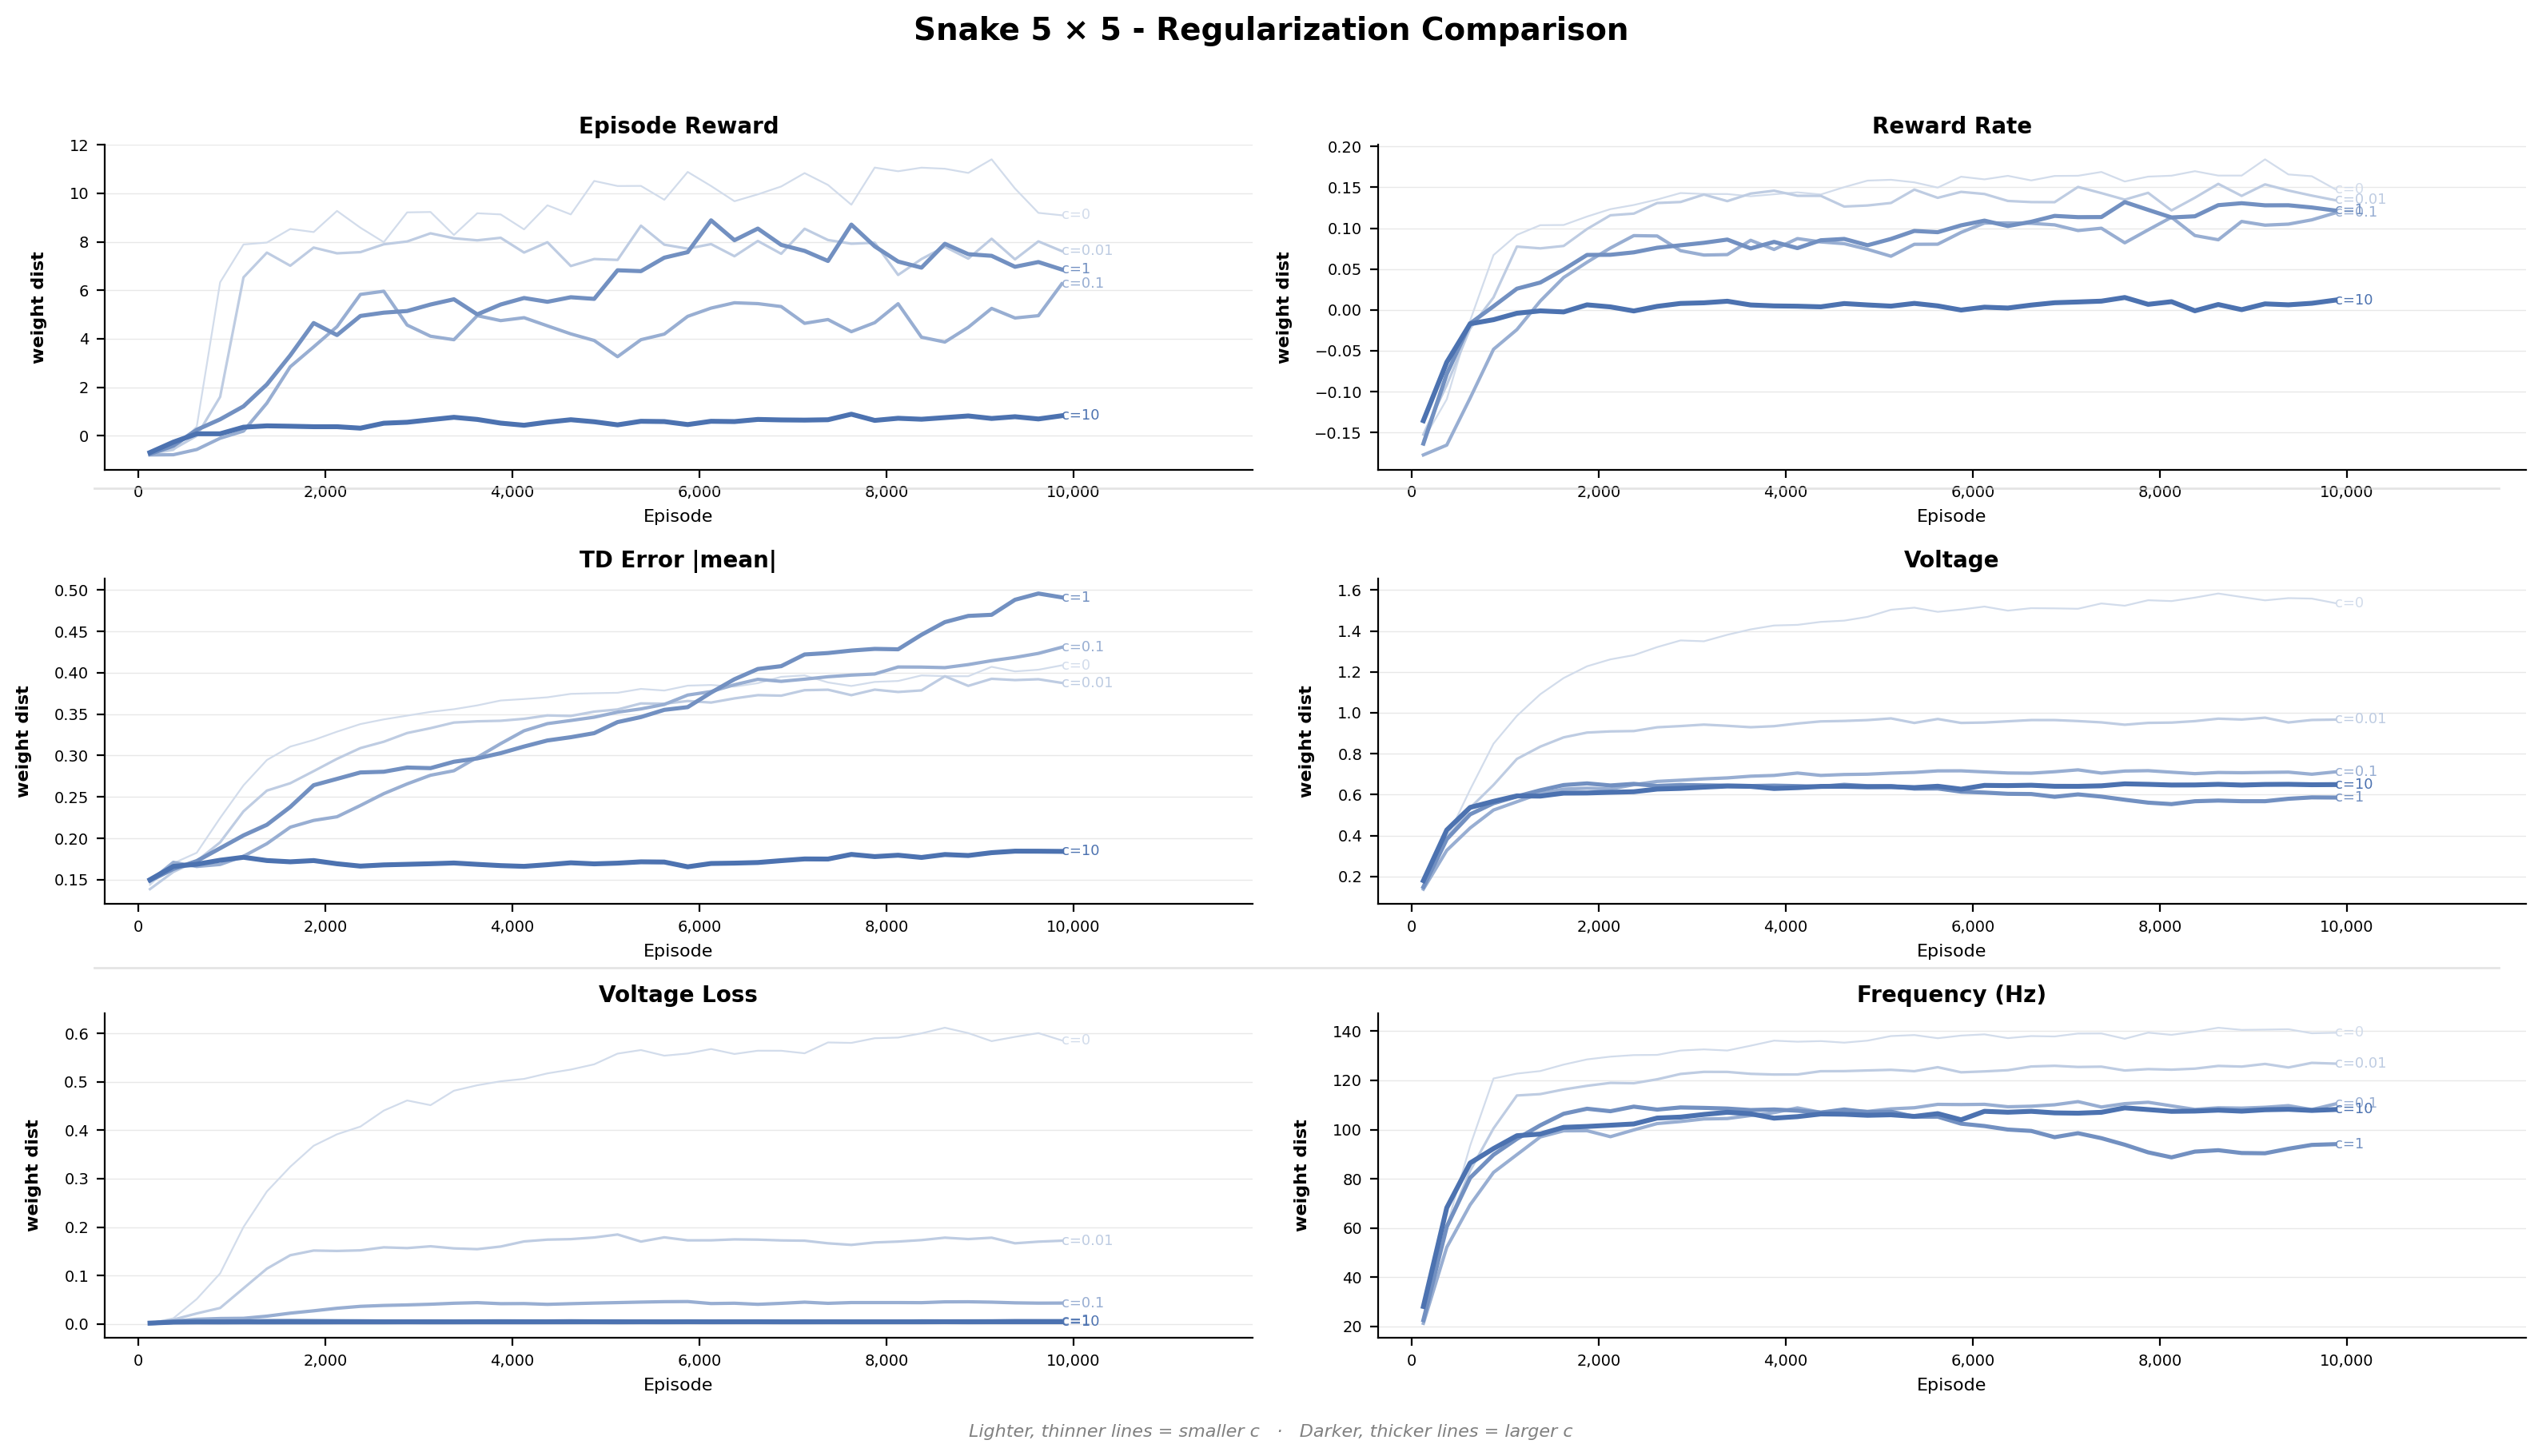
\includegraphics[width=1\linewidth]{images/SnakeRegularizationComparison.png}
    \caption[Reward-based regularization sweep (Snake)]{Reward-based regularization comparison for \emph{weight dist}
    on Snake $5 \times 5$, sweeping over regularization strength $c_{reg}$
    (lighter, thinner lines correspond to smaller values, darker thicker
    lines to larger values). Each panel reports one of the six standard
    metrics over $10,000$ episodes.}
    \label{fig:snake-regularization}
\end{figure}

\section{Best Individual Performances on Snake $5\times5$}

\begin{table}[H]
\caption{Snake results sorted by best mean of 100 Scores (highest to lowest) and Best mean of 100 episode Reward Rates. Each individual run belongs to an experiment, when the name is of the form \emph{variant}($x$) it belongs to the comparative result, otherwise the name discriminates which experiment it belongs to}
\label{tab:snake-best100-score}
\begin{tabular}{l r r r r}
\hline
File & Best100 RewardRate & Best100 Score & Wins & Win \% \\
\hline
symmetric                             & \textbf{0.2113} & \textbf{12.6500} & 14 & 0.1400 \\
weight dist creg 0 (Reg Comp)         & 0.1897 & 12.3100 & \textbf{33} & \textbf{0.3300} \\
weight dist(4)                        & 0.1823 & 11.8200 & 11 & 0.1100 \\
weight dist(3)                        & 0.1776 & 11.7300 & 8  & 0.0800 \\
combined(3)                            & 0.1868 & 11.6000 & 13 & 0.1300 \\
combined lambda 08                     & 0.1761 & 11.5600 & 8  & 0.0800 \\
combined(5)                            & 0.1826 & 11.5100 & 14 & 0.1400 \\
combined(1)                            & 0.1792 & 11.4500 & 6  & 0.0600 \\
adaptive lambda 09                     & 0.1858 & 11.2100 & 3  & 0.0300 \\
adaptive(4)                            & 0.1795 & 11.1300 & 14 & 0.1500 \\
combined(2)                            & 0.1816 & 11.0100 & 11 & 0.1100 \\
weight dist layers 1                   & 0.1755 & 10.9800 & 7  & 0.0700 \\
weight dist(5)                         & 0.1755 & 10.9800 & 7  & 0.0700 \\
adaptive(3)                            & 0.1844 & 10.6500 & 11 & 0.1100 \\
adaptive layers 1                      & 0.1870 & 10.6100 & 5  & 0.0500 \\
weight dist(1)                         & 0.1704 & 10.6100 & 3  & 0.0300 \\
weight dist(2)                         & 0.1743 & 10.5700 & 3  & 0.0300 \\
adaptive lambda 08                     & 0.1816 & 10.5500 & 7  & 0.0700 \\
adaptive lambda 07                     & 0.1808 & 10.4600 & 8  & 0.0800 \\
adaptive(5)                            & 0.1772 & 10.4200 & 7  & 0.0800 \\
adaptive lambda 06                     & 0.1694 & 10.4100 & 6  & 0.0600 \\
combined lambda 07                     & 0.1770 & 10.1900 & 3  & 0.0300 \\
combined(4)                            & 0.1729 & 10.1300 & 6  & 0.0600 \\
weight dist creg 001 (Reg Comp)        & 0.1689 & 9.6000  & 4  & 0.0400 \\
adaptive lambda 04                     & 0.1709 & 9.5800  & 6  & 0.0600 \\
\hline
\end{tabular}
\end{table}

As expected the best metrics belong to the \emph{symmetric} variant, but surprisingly the version of \emph{weight dist} with no regularization beats by a factor of 2.36 in the number of wins and gets very close to the other metrics of the \emph{symmetric} variant.

Here, without taking into account the \emph{symmetric} variant we see that the \emph{combined} rules reliably get to high rewards and win rates, the \emph{adaptive} variant seems to get close to combined, but notably the two top runs do not belong to either \emph{adaptive} nor \emph{combined}, the best two runs, disregarding \emph{symmetric}, are of \emph{weight dist}. This could be because this method has higher variance in the strategies it discovers, and therefore in the rewards it gets, and the other two might converge to more concrete strategies.

\clearpage

\section{Distributed E-prop versus Adaptive E-prop on Pac-Man with
randomized Layouts}
\label{sec:pacman_comparison}

\subsection{Comparison with $\lambda = 0.5$}
Figure~\ref{fig:pacman_comparison} shows a controlled comparison between
distributed e-prop and adaptive e-prop on the Pac-Man randomized layouts
problem, averaged over five independent runs under identical configurations.

\begin{figure}[H]
    \centering
    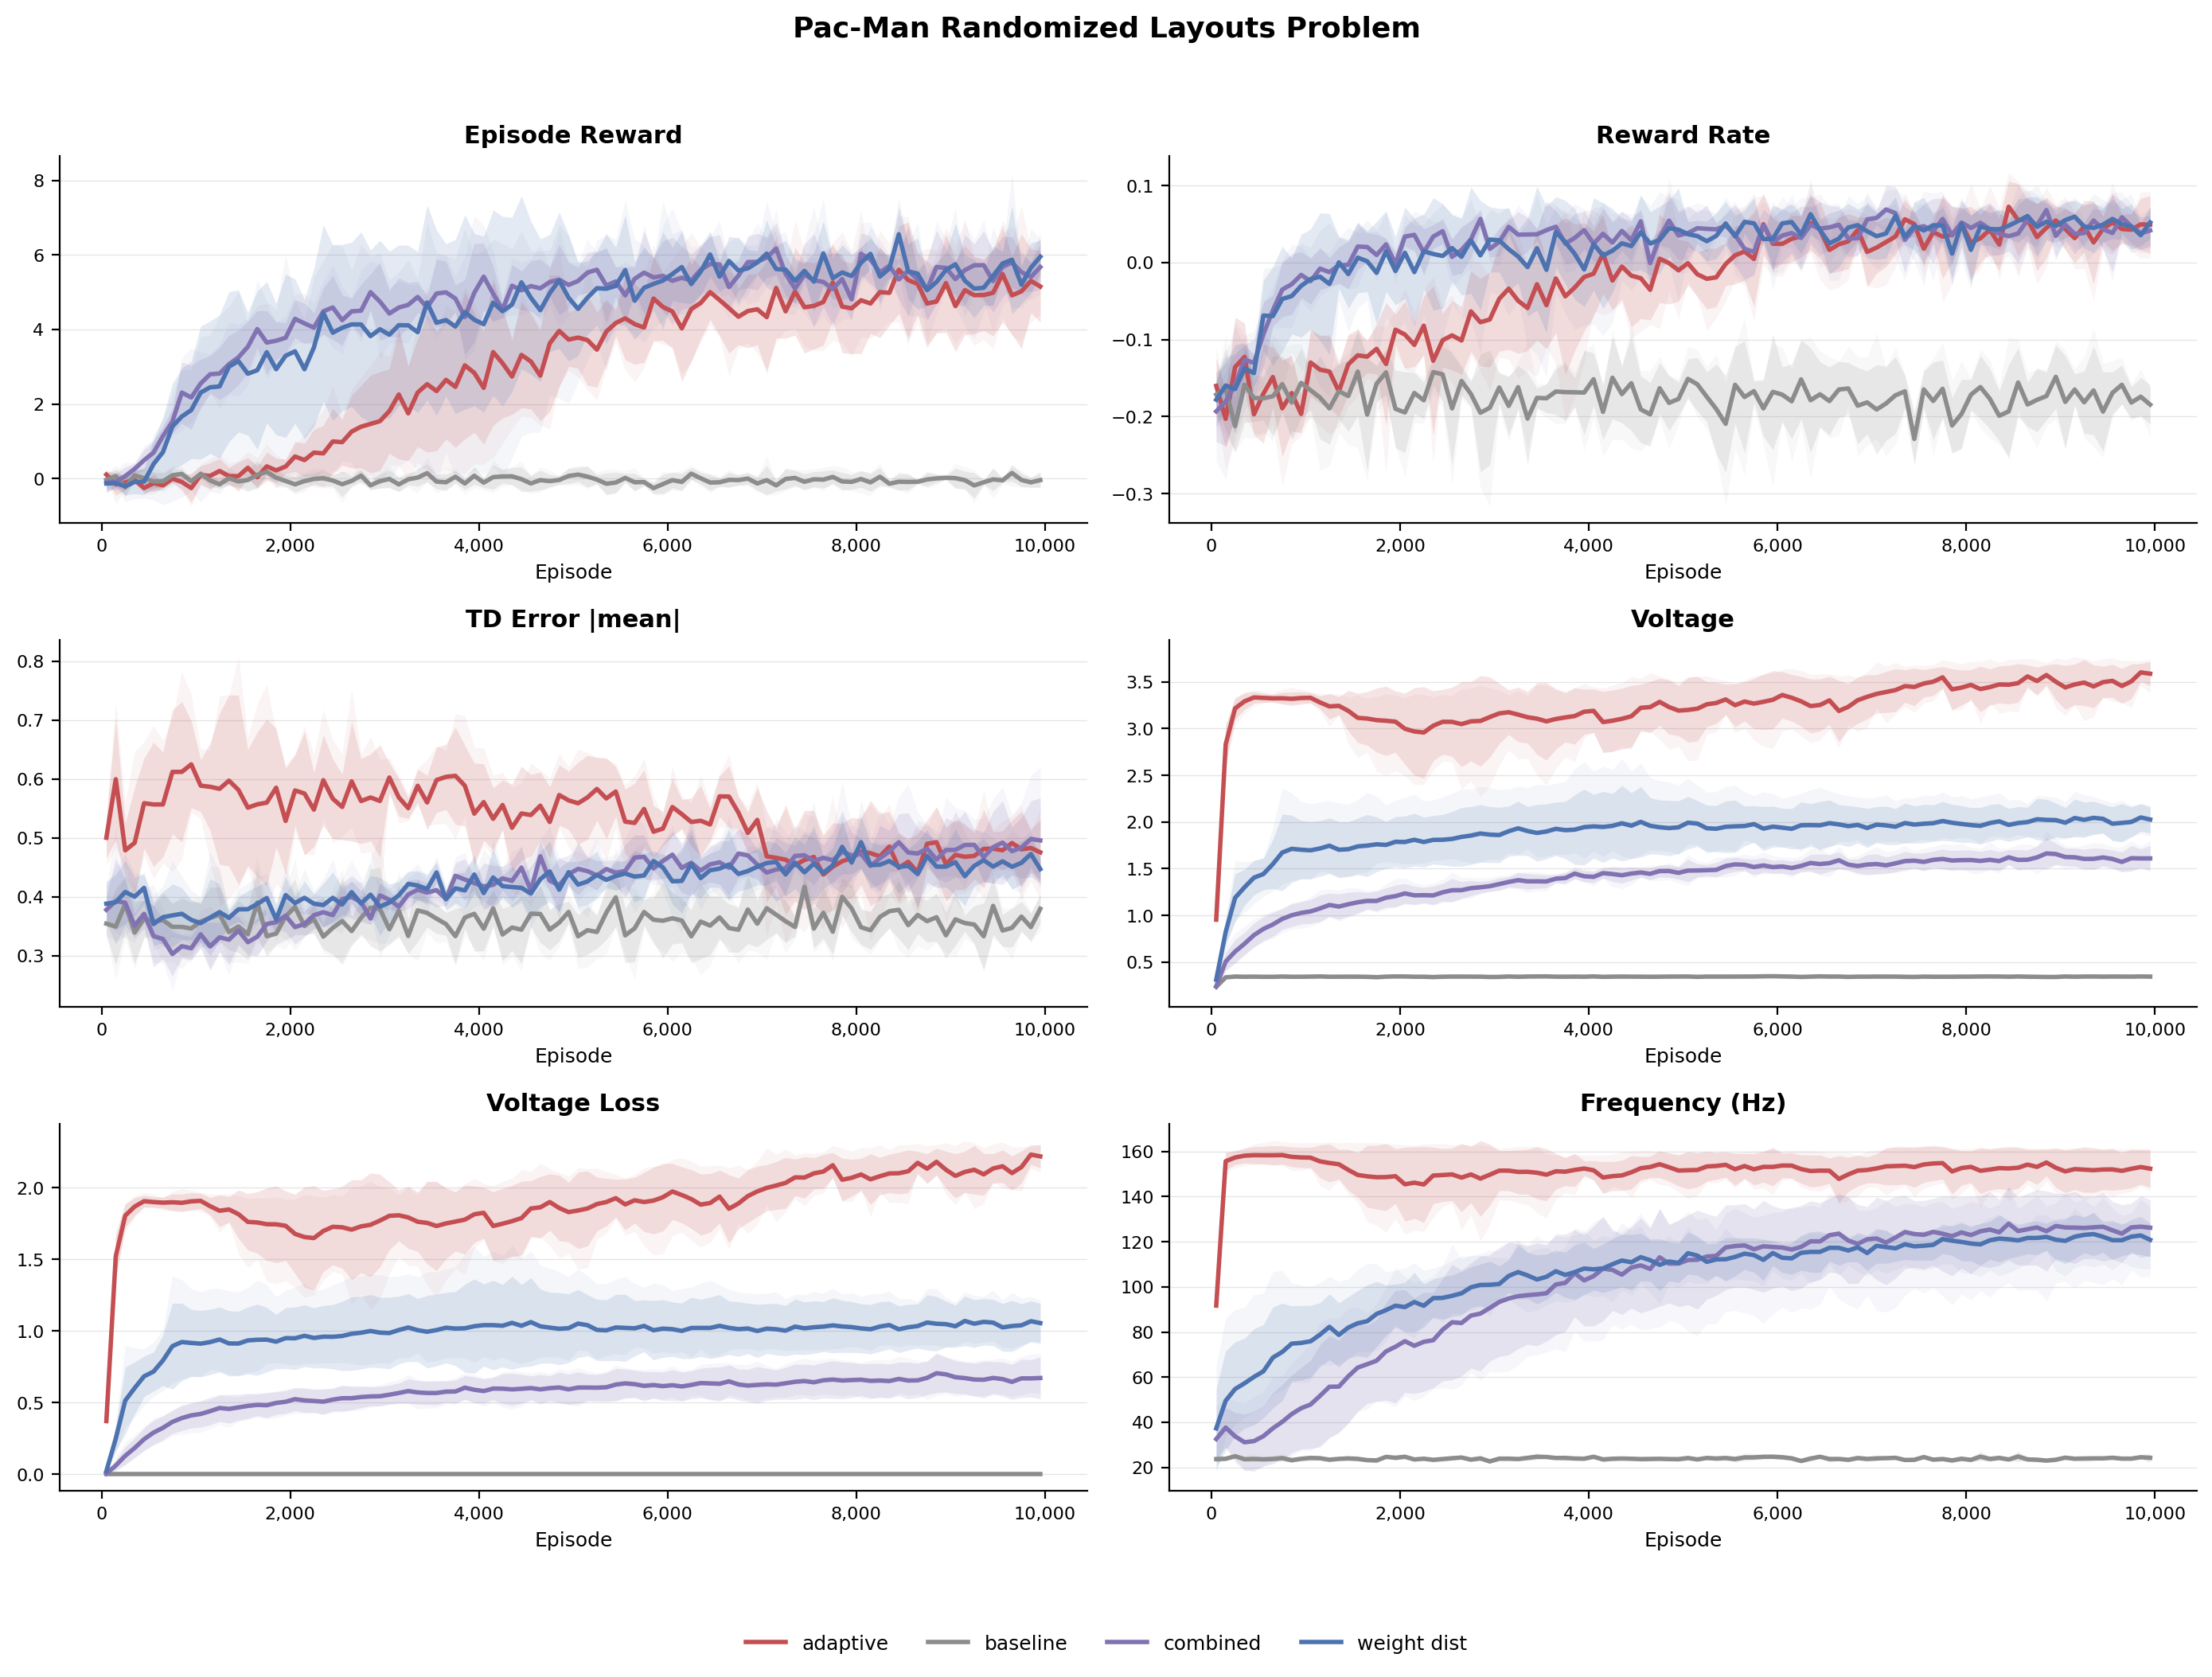
\includegraphics[width=1.0\textwidth]{images/PacManComparison.png}
    \caption[Distributed vs.\ adaptive e-prop (Pac-Man)]{Controlled comparison of distributed e-prop variants and
    adaptive e-prop on the Pac-Man randomized layouts problem, averaged
    over five independent runs with shaded standard deviation bands.
    Top row: episode reward and reward rate. Middle row: absolute TD
    error and mean membrane voltage. Bottom row: voltage loss and mean
    firing frequency.}
    \label{fig:pacman_comparison}
\end{figure}

Under equal conditions, distributed e-prop variants reach higher episode
rewards than adaptive e-prop, though both converge to comparable reward
rates by the end of training. The TD error is more unstable for adaptive
e-prop, and its voltage and frequency metrics are both worse and more
variable throughout training, consistent with the pattern observed in the
Snake experiments. The \emph{combined} variant again behaves more
similarly to the distributed e-prop family than to adaptive e-prop across
all metrics, reinforcing the observation from
Section~\ref{sec:snake_comparison} that its update is dominated by the
perturbation-based signal in this implementation.

A further limitation of these results is the length of the experiments.
Both algorithms show signs of continued improvement at the end of the
10,000 episode training horizon, particularly in the reward rate plots,
suggesting that the performance gap between them could narrow or widen
further with longer training. The conclusions drawn here should therefore
be understood as reflecting behavior within this specific training budget.

Taken together, these results reinforce the picture that emerged from the
Snake experiments: distributed e-prop and adaptive e-prop make different
assumptions about the network dynamics, exploit different sources of credit
assignment information, and appear to thrive under different operating
conditions. Understanding when and why one outperforms the other remains
an important open question that a more systematic study varying neuron
configuration, network size, task structure, and training length would be
needed to resolve.

The baseline, as in snake stays flat on all metrics, not learning at all.

Figure~\ref{fig:value_function_comparison} provides a qualitative view of
the value function learned by each algorithm at three different stages of
training, from earlier episodes at the top to later episodes at the bottom.

\begin{figure}[H]
    \centering
    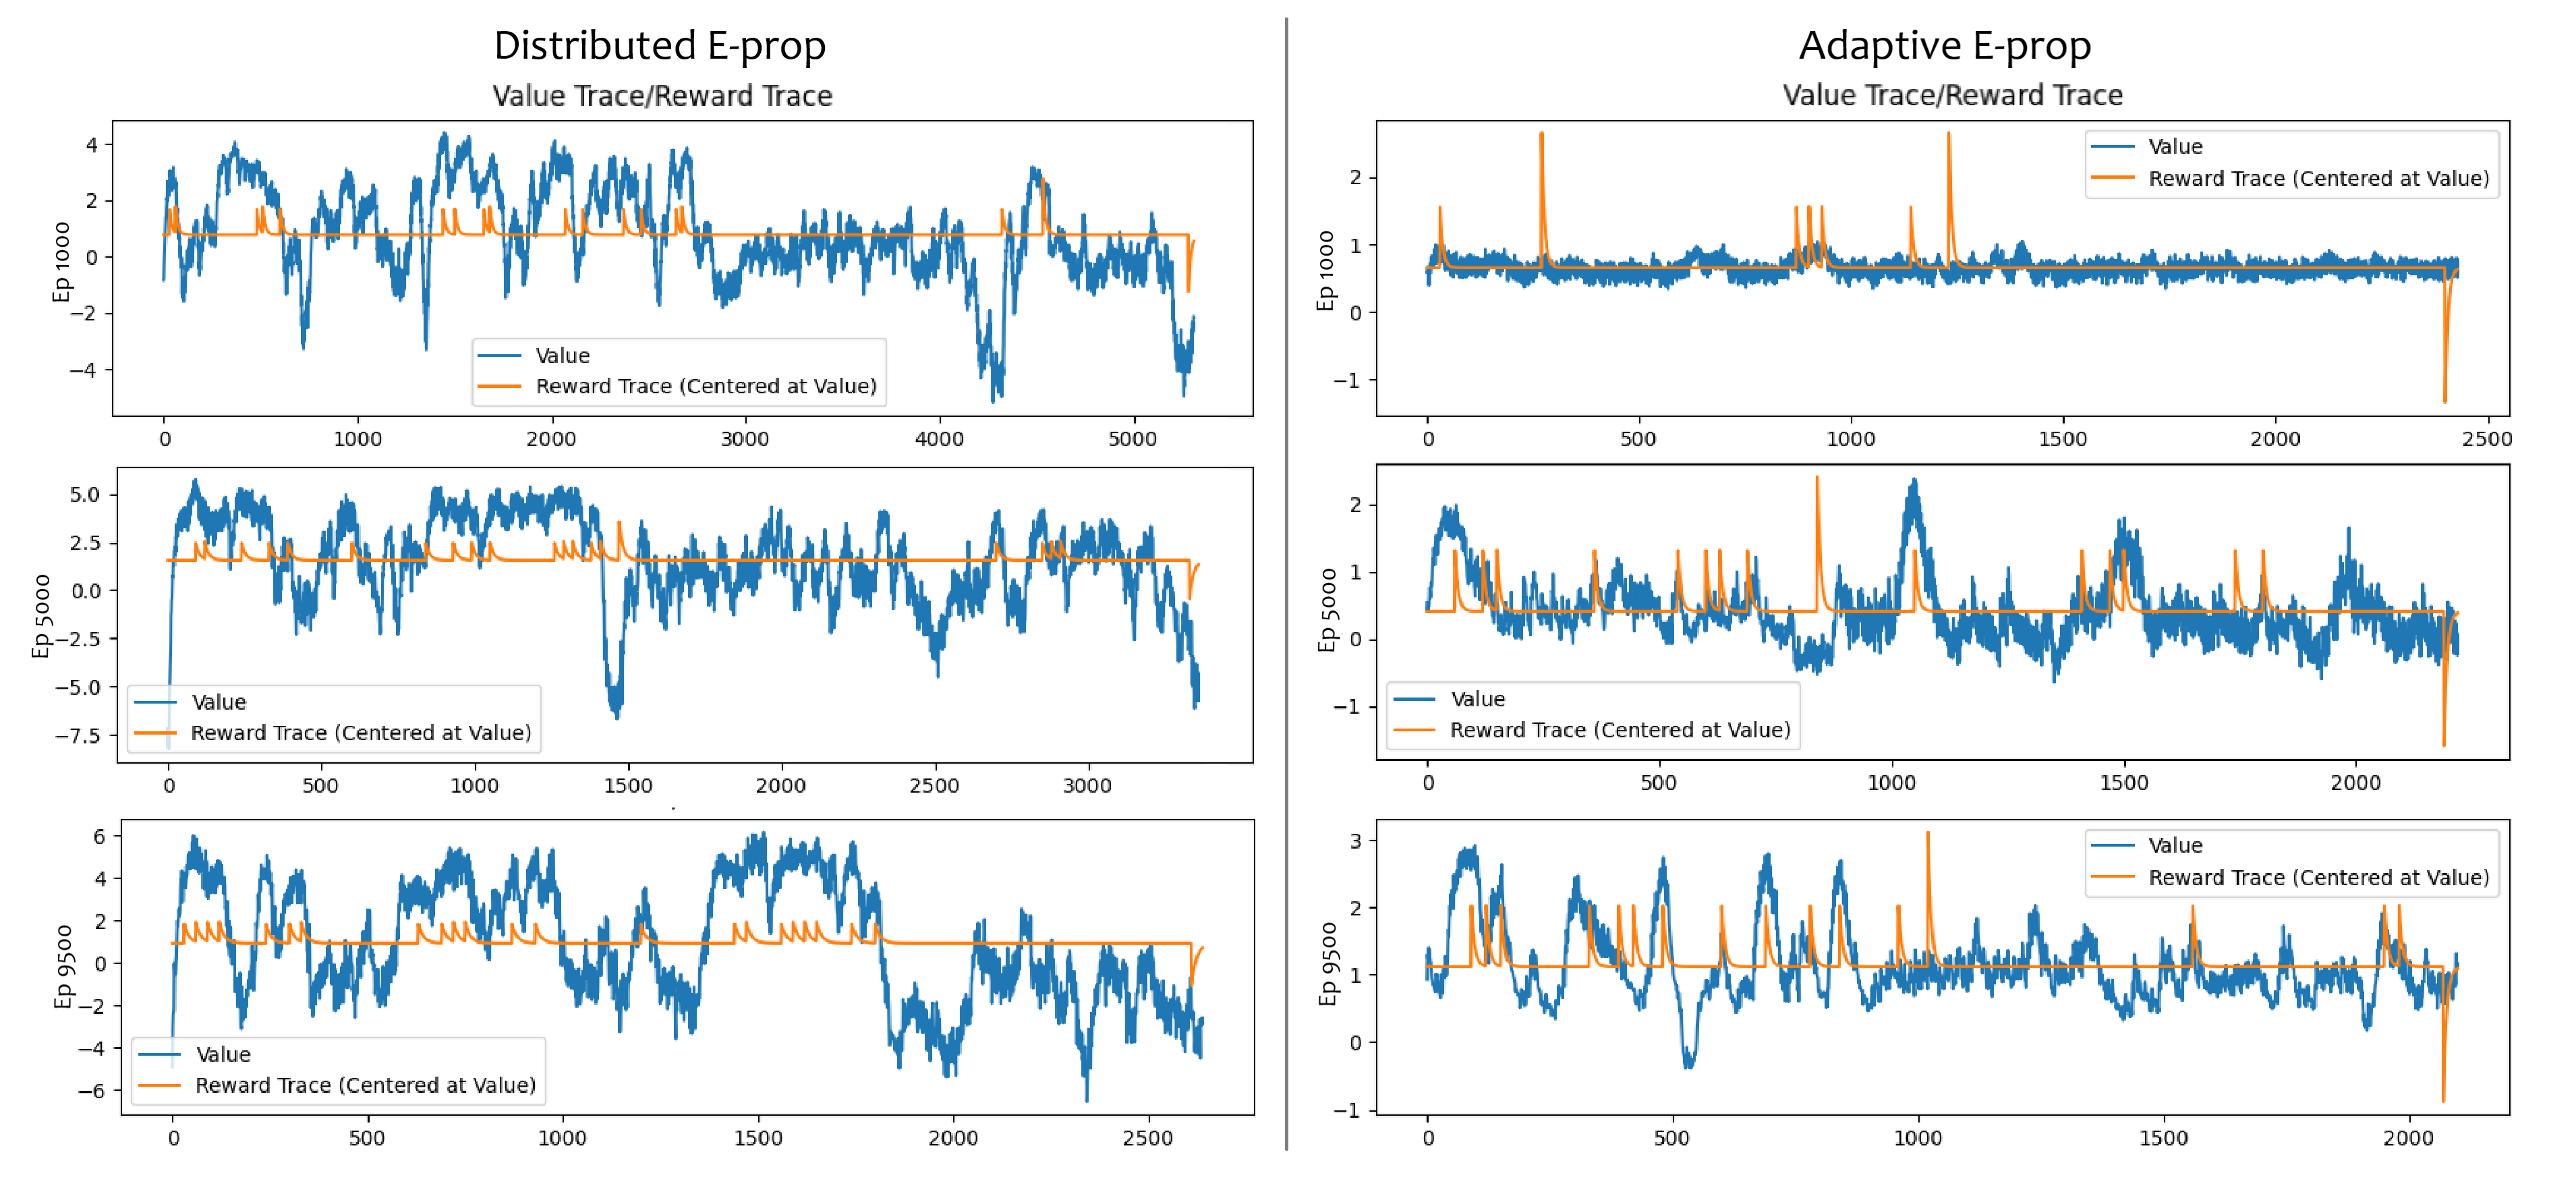
\includegraphics[width=1.0\textwidth]{images/ValueFunctionPacManComparison.png}
    \caption[Value traces: distributed vs.\ adaptive e-prop (Pac-Man)]{%
    Value function and centered reward trace for distributed e-prop (left) and
    adaptive e-prop (right) on Pac-Man, at three stages of a single training run,
    ordered from earlier (top) to later (bottom). As in the Snake value-trace
    figure, the two axes measure different things: down a column the rows are
    separate training snapshots, not one continuous signal, while across a panel the
    horizontal axis is the frame number within a single game at that stage, and
    restarts from zero, so panels spanning games of different lengths differ in
    width. The blue trace is the learned value estimate $V_t$; the orange trace is
    the reward trace, shifted to sit at the value level so
    that reward events can be read directly against the value. Vertical scales are
    independent per panel, since the magnitude of the learned value grows over
    training.}
    \label{fig:value_function_comparison}
\end{figure}

Across all three stages of training, the value function learned by
distributed e-prop tracks the reward trace more closely and with greater
dynamic range than that of adaptive e-prop, which remains comparatively
flat and close to a constant baseline throughout training. This mirrors
what was observed in the Snake experiments, and is again at odds with the
TD error plots: the absolute TD error grows over the course of training
for distributed e-prop while decreasing for adaptive e-prop. As discussed
in Section~\ref{sec:snake_comparison}, a flat value function naturally
produces small TD errors without necessarily carrying useful information,
while a more expressive and dynamic estimate will make larger predictions
that can be more wrong on any given step. The TD error should therefore
not be read as a measure of critic quality in isolation, and this
observation is particularly clear here.

An example of the richer value representation learned
by distributed e-prop can be seen in the traces, where on several occasions
the value estimate drops sharply into negative territory immediately before
a large positive reward spike of magnitude 2, corresponding to the agent
eating a frightened ghost. This indicates that the agent expected to die
in that moment, likely because it was in close proximity to the ghost, but
instead managed to eat it. The critic has evidently learned to associate
ghost proximity with danger, which is a meaningful and correct association in most
circumstances, but one that fails to account for the capsule state that
makes the ghost vulnerable. This kind of structured but imperfect prediction
is only possible if the value function has learned something genuine about
the task dynamics, and it stands in clear contrast to the flat adaptive
e-prop estimates which neither anticipate danger nor respond to the
ghost-eating reward in any structured way.

\subsection{No Integration During Refractory Period}
\label{subsec:no_refractory_integration}

\begin{figure}[htpb]
    \centering
    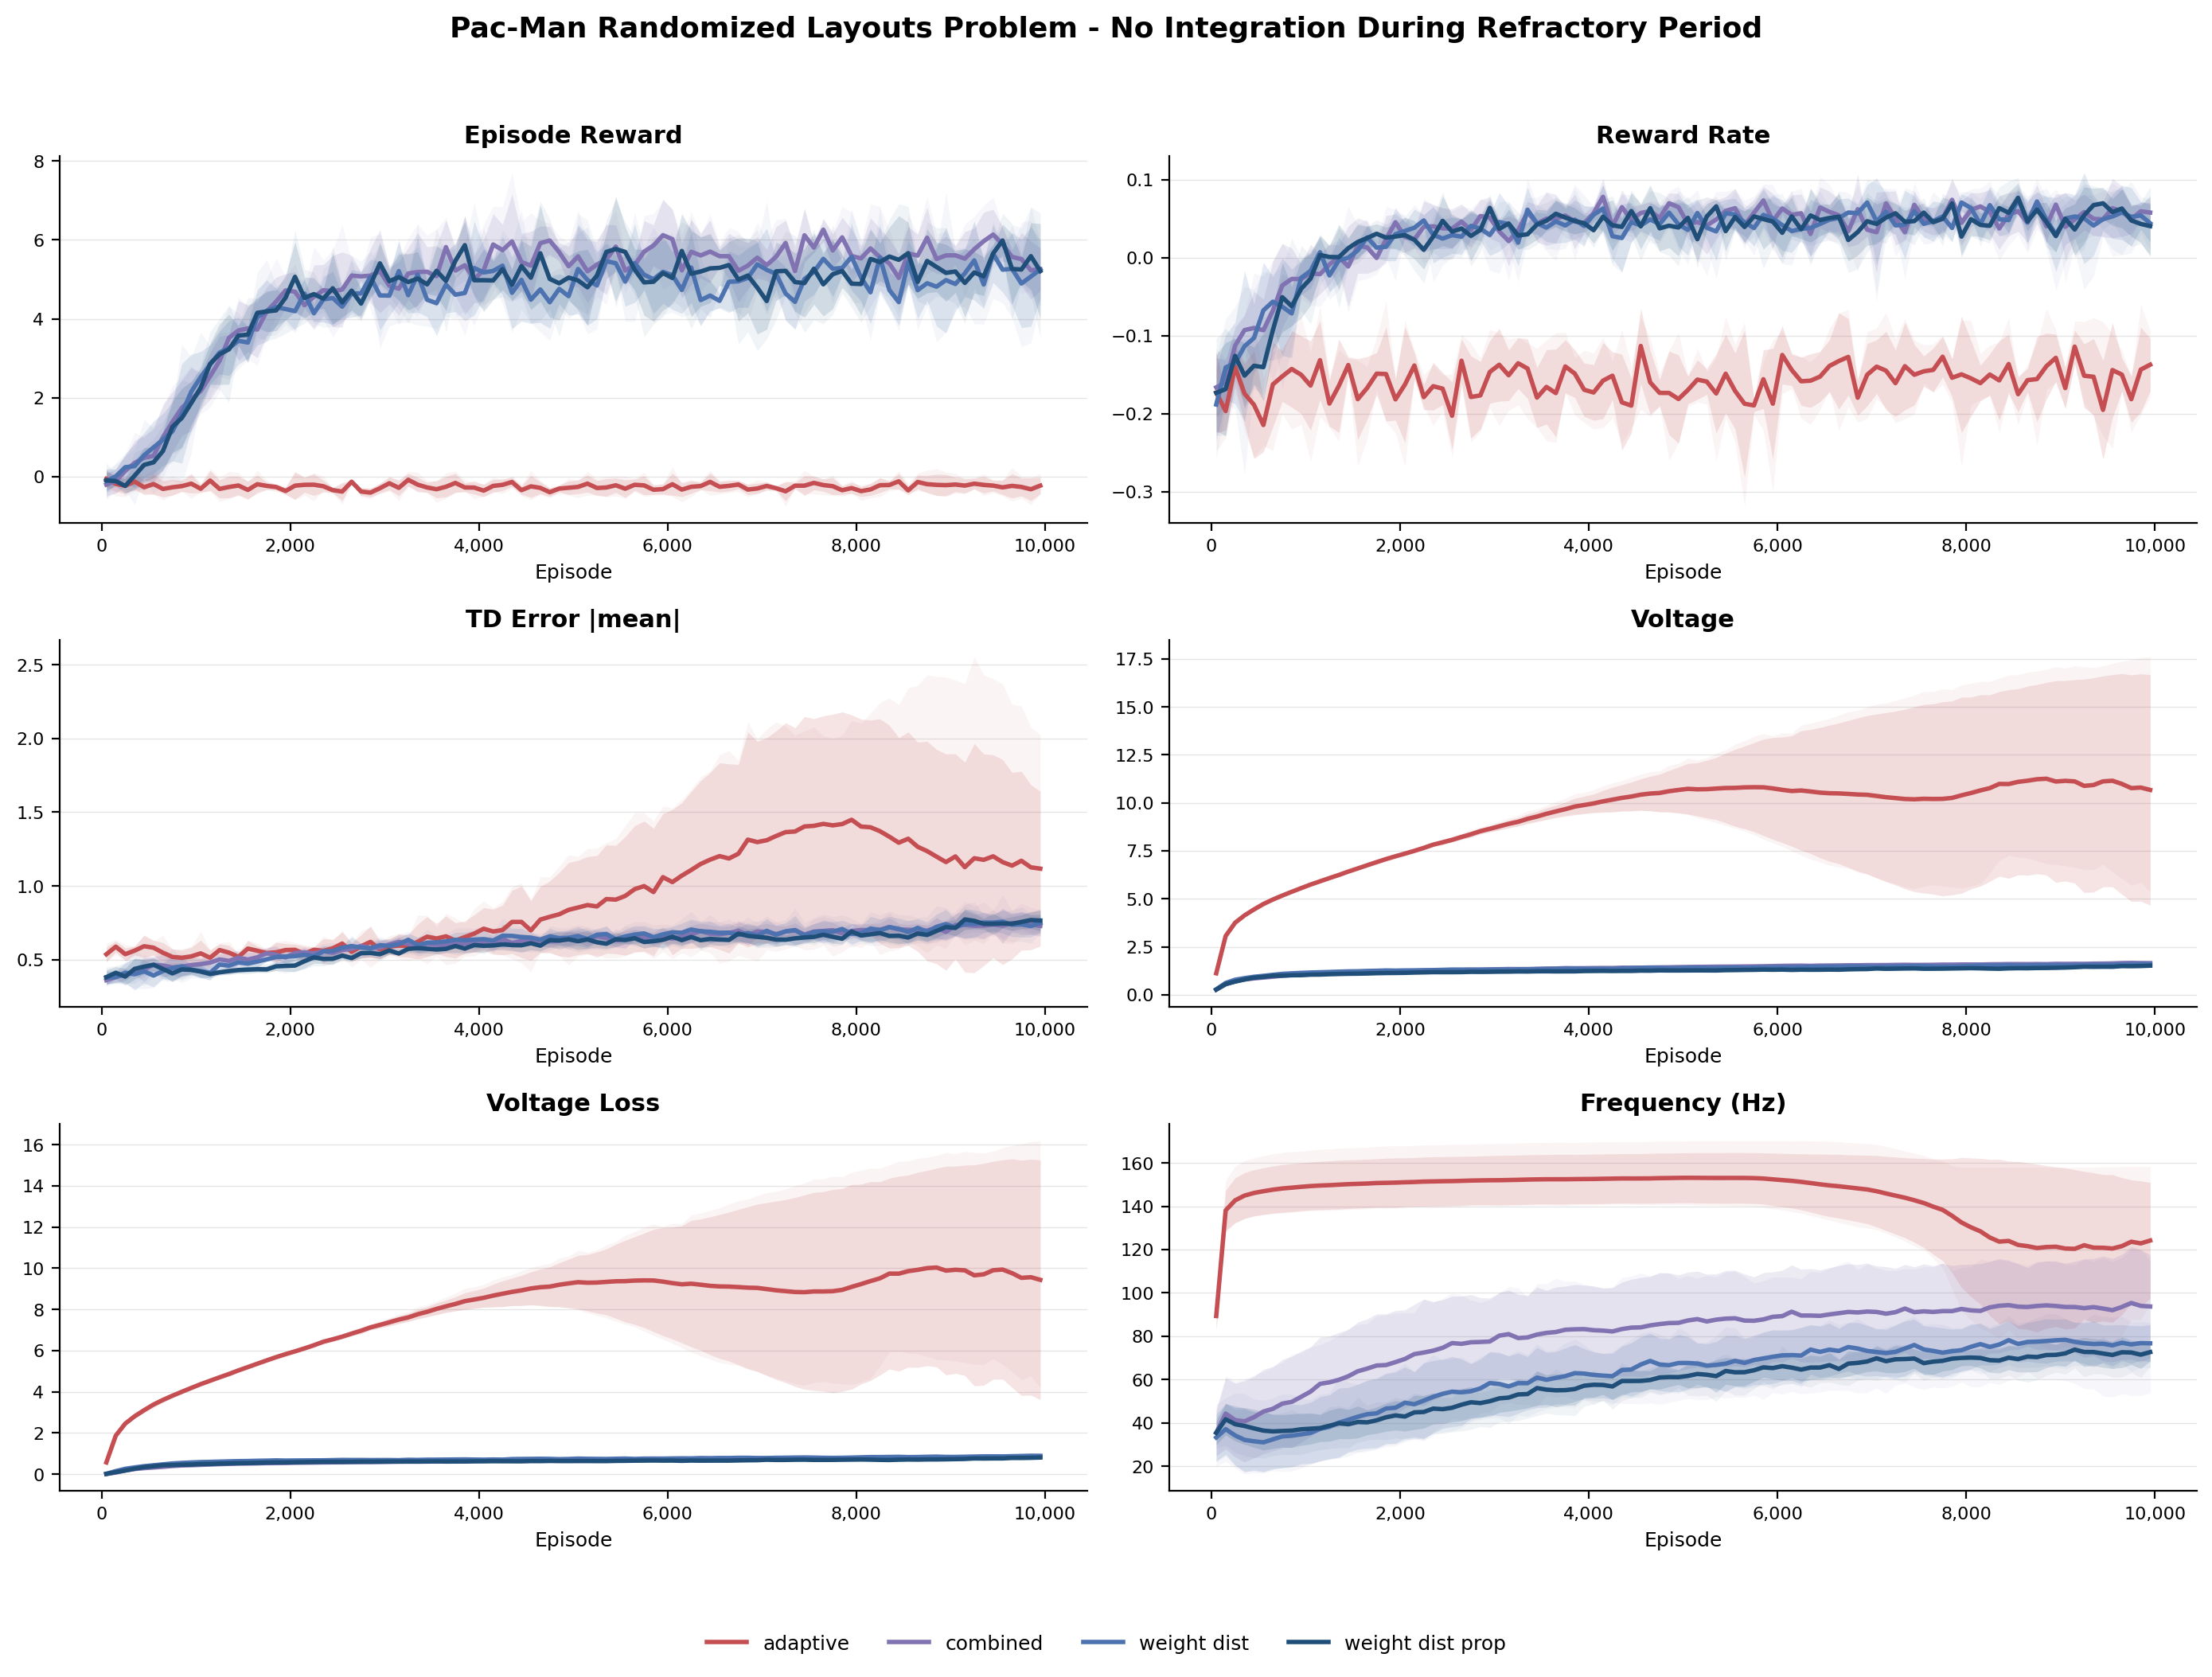
\includegraphics[width=1.0\textwidth]{images/PacManComparisonNoIntegration.png}
    \caption[No-refractory-integration comparison (Pac-Man)]{Comparison of distributed e-prop variants and adaptive e-prop
    on the Pac-Man randomized layouts problem under the
    no-integration-during-refractory-period neuron variant, with reward
    trace decay set to 0.1 for all variants, averaged over five independent
    runs with shaded standard deviation bands. Top row: episode reward and
    reward rate. Middle row: absolute TD error and mean membrane voltage.
    Bottom row: voltage loss and mean firing frequency.}
    \label{fig:pacman_no_integration}
\end{figure}

This experiment runs both algorithms under the neuron variant that does not integrate inputs during the refractory period, with the reward trace decay set to 0.1 for all variants. Standard
e-prop handles this variant poorly, its eligibility trace derivation assumes
integration continues during the refractory period, and violating this
assumption introduces inconsistencies between the forward dynamics and the
learning rule. Distributed e-prop is less sensitive to this assumption since
its credit assignment is based on perturbation correlations rather than on
a precise analytical decomposition of the gradient.

The results reflect this difference clearly. Adaptive e-prop barely learns
under this configuration, with episode reward remaining near zero and
voltage and frequency metrics diverging severely throughout training. The
distributed e-prop variants, by contrast, learn the task successfully and
maintain well-regulated spiking dynamics. Among them, \emph{combined}
achieves marginally higher episode rewards but at the cost of worse
frequency metrics, while \emph{weight dist prop} finds less active
configurations than both \emph{combined} and \emph{weight dist} while
maintaining comparable task performance. This contrasts with the Snake
results in Section~\ref{sec:snake_comparison}, where structured routing
was clearly detrimental to \emph{weight dist}; here it appears to find
sparser activity patterns that are sufficient for the task, though we do
not offer a mechanistic explanation for this difference.

The advantage of distributed e-prop in this setting is not merely a
consequence of a more favorable hyperparameter configuration; it reflects
a genuine difference in how the two rules interact with the network
dynamics when the refractory period assumption is violated. Whether this
robustness extends to other neuron variants or network configurations
remains an open question.

\subsection{Lambda Comparison}
\label{subsec:pacman_lambda_comparison}

Figure~\ref{fig:pacman_lambda} repeats the decay-factor sweep introduced in
Section~\ref{sec:snake_lambda_comparison} on the Pac-Man randomized layouts
problem, this time comparing adaptive e-prop and the structured-routing
distributed variant \emph{weight dist prop}. As anticipated there, the
two tasks produce markedly different pictures of which learning rule
tolerates a wide range of $\lambda$, and it is this contrast, that is most informative.

The distributed variant used throughout this comparison is run under the
\emph{no-integration-during-refractory-period} neuron variant introduced in
Section~\ref{subsec:no_refractory_integration}. This choice is
deliberate: among the configurations evaluated on the Pac-Man randomized
layouts problem, this variant was one of the strongest performers for 
the distributed eprop variants, and it also produced the most favorable
voltage and frequency statistics of the configurations tested, remaining
well-regulated where the standard-refractory configuration showed more
pronounced drift. Using this variant for the $\lambda$ sweep therefore
gives distributed e-prop a comparatively stable starting point from which
to isolate the effect of $\lambda$ specifically. Adaptive
e-prop, by contrast, is shown here under its standard configuration, since
Section~\ref{subsec:no_refractory_integration} found this same neuron variant
to be markedly detrimental to adaptive e-prop; the
two algorithms are therefore each shown under the neuron configuration
most favorable to them individually, which should be kept in mind when
comparing the absolute stability of their voltage and frequency curves
below.

\label{sec:lambda_comparison}
\begin{figure}[htbp]
    \centering
    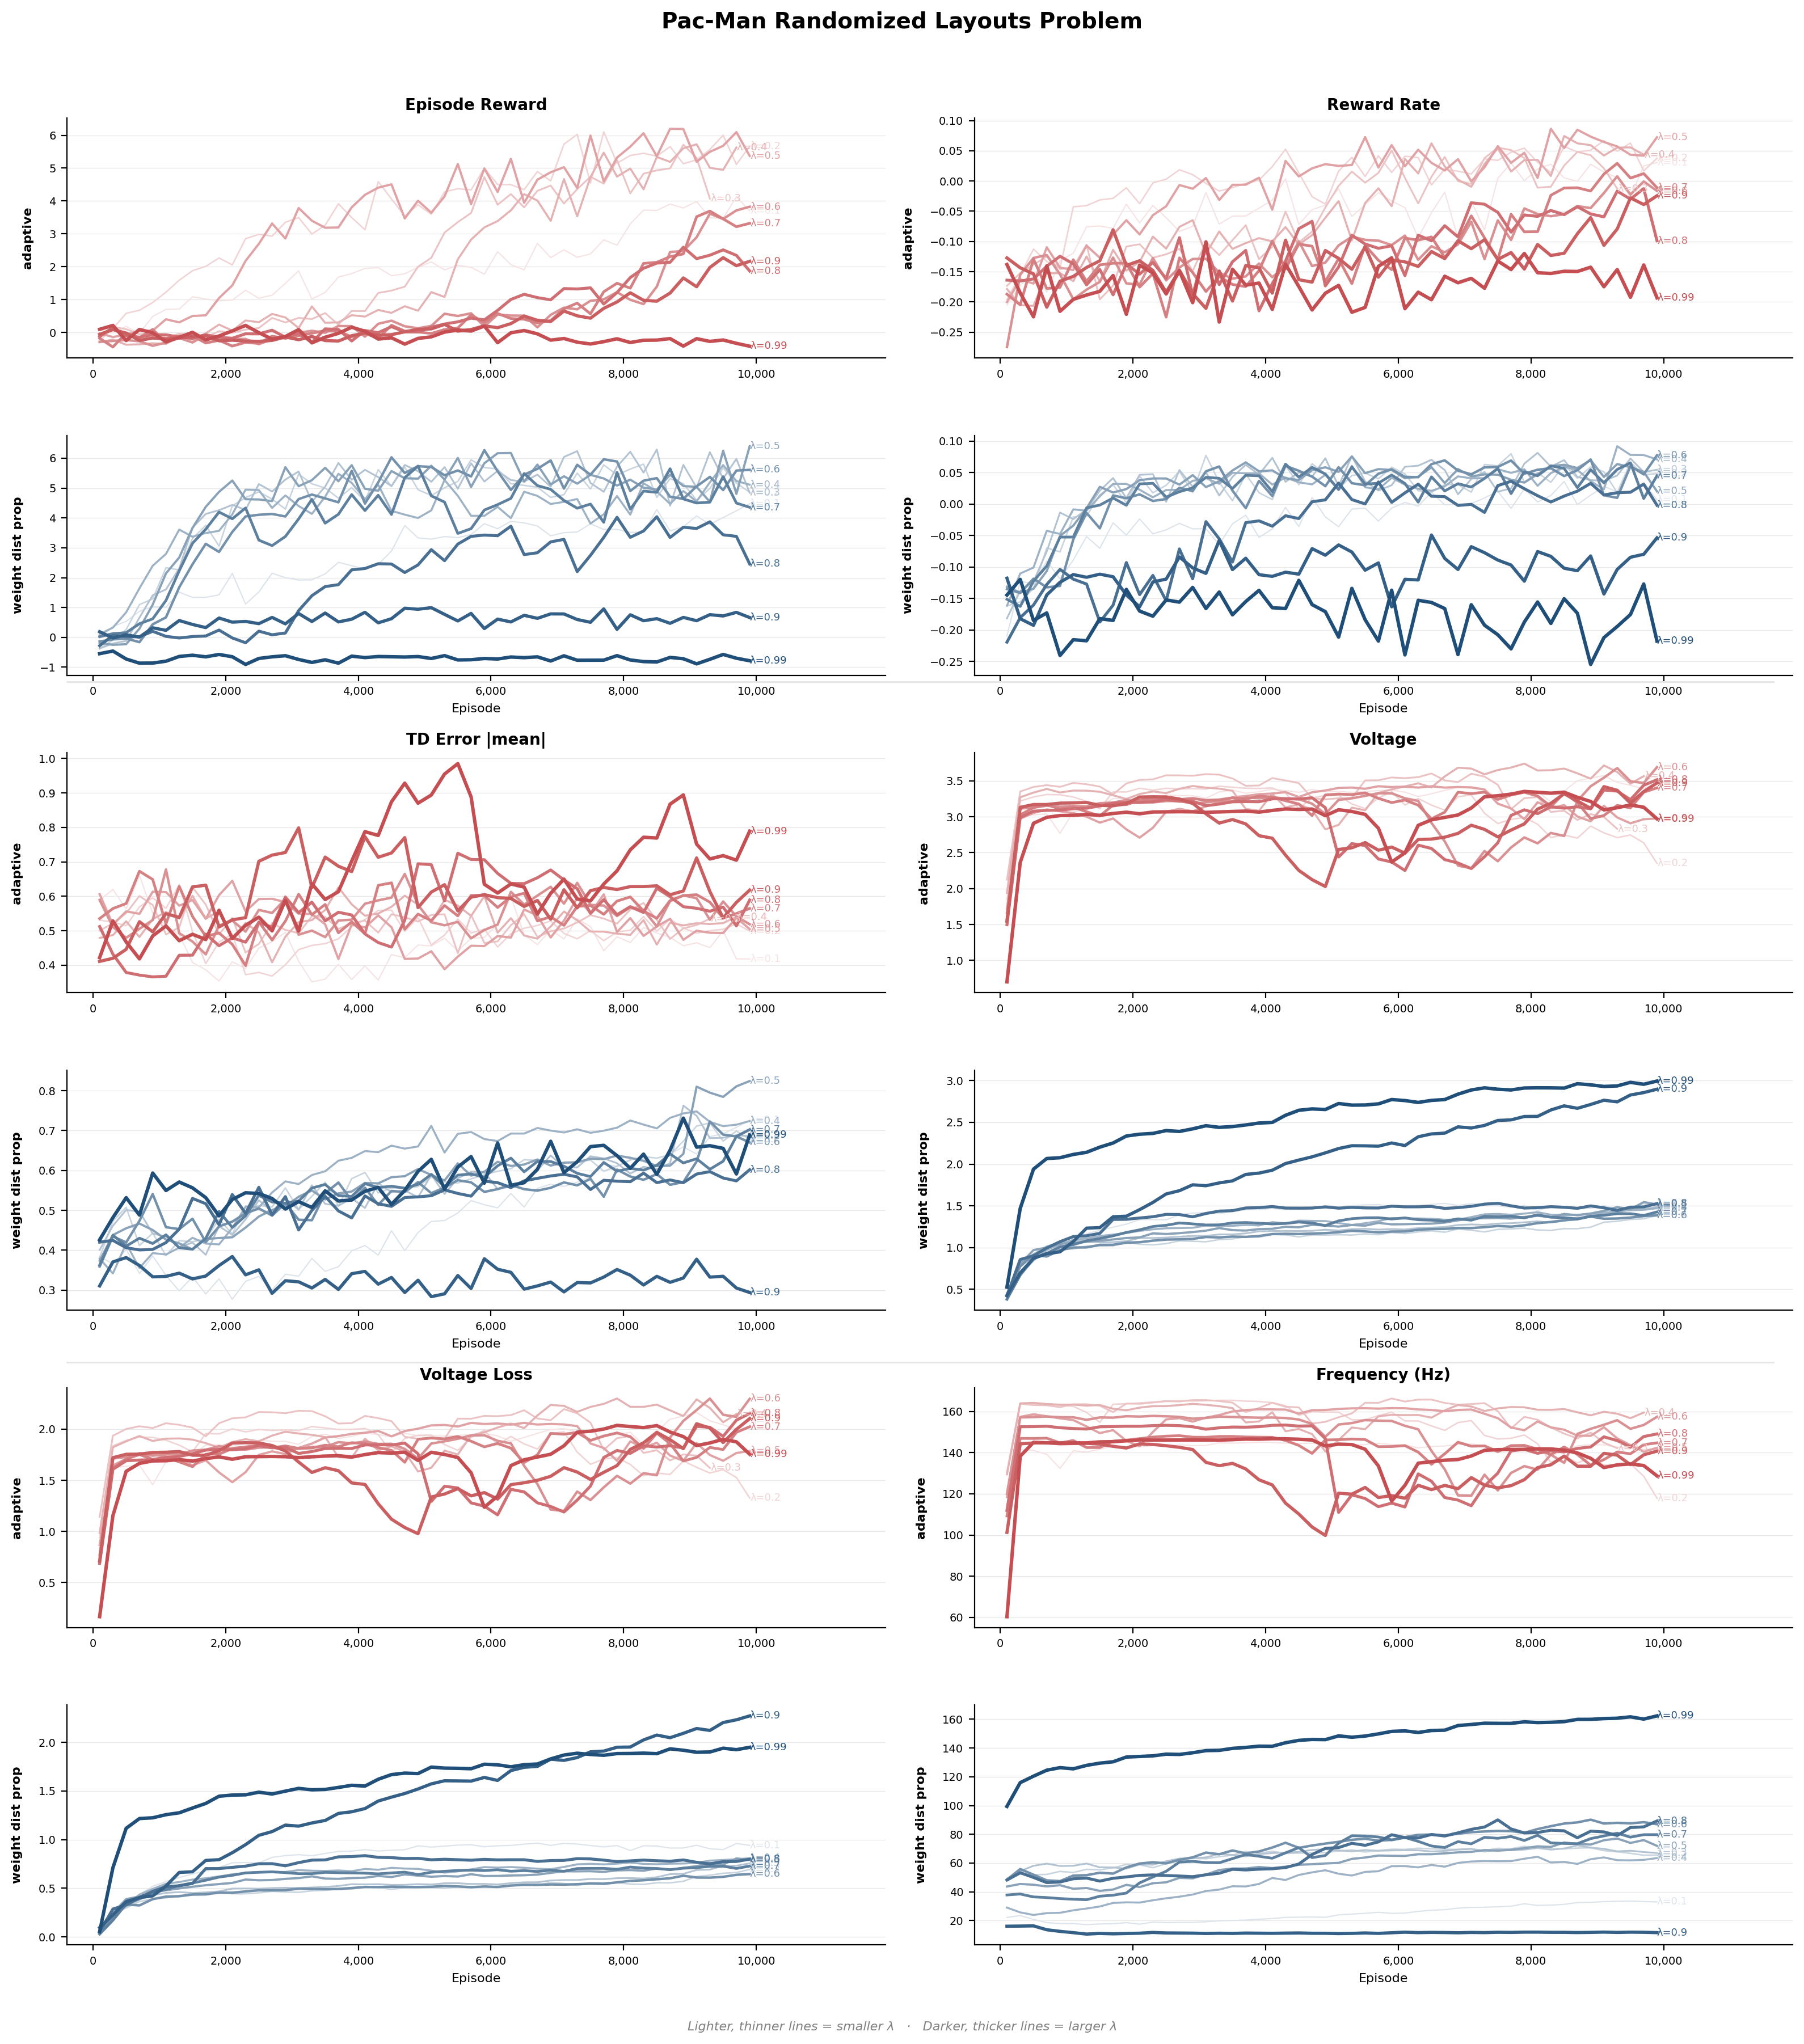
\includegraphics[width=\textwidth]{images/PacManComparisonLambdaGroups.png}
    \caption[Lambda sweep on Pac-Man]{Training performance across $10,000$
    episodes on the Pac-Man randomized layouts problem for adaptive e-prop
    (red) and \emph{weight dist prop} (blue), across varying decay
    factors $\lambda \in \{0.1, 0.2, \ldots, 0.9, 0.99\}$ (lighter, thinner
    lines correspond to smaller $\lambda$; darker, thicker lines to larger
    $\lambda$). Metrics reported include episode reward, reward rate, TD
    error (mean), voltage, voltage loss, and frequency (Hz).}
    \label{fig:pacman_lambda}
\end{figure}
For both algorithms, the best episode reward and reward rate are reached
around $\lambda = 0.5$, with performance generally falling off as
$\lambda$ increases. As
discussed in Section~\ref{sec:snake_lambda_comparison}, a larger $\lambda$
trades a longer credit-assignment reach for a higher-variance trace, and
on this task a short horizon already appears sufficient to capture the
relevant action-reward delays, so little is gained, and much is lost, by
extending it further. The more informative difference between the two
rules lies not in where the optimum falls but in the \emph{shape} of
learning across the sweep, and in this respect the picture is the reverse
of what was seen on Snake. Adaptive e-prop shows a markedly inconsistent
onset of learning across $\lambda$ values: several of its curves remain
flat for an extended initial period before rising, echoing the slow,
feedback-alignment-dependent start already observed in
Section~\ref{subsec:snake-depth-comparison}, with no clear relationship between
$\lambda$ and how long this initial delay lasts. The distributed variant,
by contrast, begins improving promptly across most of the sweep, with
$\lambda \in \{0.4, 0.5, 0.6\}$ all reaching comparable, strong performance
early in training. The clear losers for distributed e-prop in this run are
the larger values $\lambda \in \{0.8, 0.9, 0.99\}$, which trail the rest of
the sweep throughout training.

Interestingly, these three under-performing runs do not all fail in the
same way. The voltage and frequency panels show that the $\lambda = 0.8$
and $\lambda = 0.99$ runs drift toward the same runaway, pathologically
high-voltage and high-frequency regime, climbing steadily across training
instead of converging. The $\lambda = 0.9$ run, however, moves in the
opposite direction, with voltage and firing frequency trending lower. 
Both extremes are consistent with the 
loss of useful credit-trace information at a poorly
chosen $\lambda$, but they point to two distinct failure modes available
to this learning rule: one in which the network drifts toward saturated,
uninformative firing, and another in which it drifts toward excessive
silence and equally uninformative activity. Because this comparison
reflects a single run per $\lambda$ value, in the same sense already
flagged for the $\lambda = 0.4$ failure of \emph{combined} on Snake in
Section~\ref{sec:snake_lambda_comparison}, we cannot determine from this
experiment alone whether $\lambda = 0.9$ reliably falls toward the
low-activity failure mode or whether this particular run simply landed on
one side of what might be a more variable outcome across seeds; it is
equally possible that a different run at $\lambda = 0.9$ would drift
toward the high-activity pathology instead, or even stabilize.
What the figure does establish is that both failure modes are reachable by
the same learning rule under similar conditions, which is itself useful to
know even without a settled account of what determines which one a given
run falls into.

Taken together with the Snake comparison in
Section~\ref{sec:snake_lambda_comparison}, these results reinforce the
view that neither learning rule is uniformly more robust to the choice of
$\lambda$. On Pac-Man, distributed e-prop tolerates a wider range of
$\lambda$ before its dynamics degrade, and begins learning consistently
once a suitable range is found, whereas adaptive e-prop's reliance on an
approximate feedback pathway appears to make its time-to-learn less
predictable across $\lambda$, independently of where its eventual
performance ceiling lies, the opposite of the ordering found on Snake. At
the same time, the divergent failure modes observed for distributed e-prop
at large $\lambda$ here indicate that its apparent robustness should not
be overstated: poor choices of $\lambda$ can still destabilise the
network, simply through more than one route, and confirming how
consistently each route is associated with a given $\lambda$ would require
repeated runs beyond the single-seed comparisons presented in this
chapter.

\section{Best Individual Performances on Pac-Man Randomized Layouts}

\begin{table}[H]
\caption{Pac-Man results sorted by best mean of 100 Scores (highest to lowest) and Best mean of 100 episode Reward Rates. Each individual run belongs to an experiment, when the name is of the form \emph{variant}($x$) it belongs to the comparative result, otherwise the name discriminates which experiment it belongs to.}
\label{tab:pacman-best100-score}
\begin{tabular}{l r r r r}
\hline
File & Best100 RewardRate & Best100 Score & Wins & Win \% \\
\hline
weight dist(1)                    & 0.1039 & \textbf{8.2030} & 10 & 0.1000 \\
weight dist(3)                    & 0.1106 & 8.1440 & 9  & 0.0900 \\
weight dist(4)                    & \textbf{0.1400} & 7.9890 & 8  & 0.0800 \\
combined (NIDRP)(3)               & 0.1075 & 7.9420 & 10 & 0.1000 \\
weight dist(2)                    & 0.1050 & 7.8270 & 4  & 0.0400 \\
adaptive(2)                       & 0.1214 & 7.8090 & 6  & 0.0600 \\
adaptive(1)                       & 0.1195 & 7.7530 & \textbf{14} & \textbf{0.1400} \\
weight dist prop lambda 03        & 0.1173 & 7.6490 & 8  & 0.0800 \\
combined(1)                       & 0.1090 & 7.6140 & 7  & 0.0700 \\
adaptive lambda 05                & 0.1228 & 7.6030 & 3  & 0.0300 \\
combined (NIDRP)(2)               & 0.1046 & 7.4820 & 5  & 0.0500 \\
combined (NIDRP)(5)               & 0.1081 & 7.4760 & 10 & 0.1000 \\
combined(3)                       & 0.1127 & 7.4470 & 4  & 0.0400 \\
combined (NIDRP)(1)               & 0.1089 & 7.4360 & 3  & 0.0300 \\
combined(4)                       & 0.1085 & 7.3770 & 4  & 0.0400 \\
weight dist prop (NIDRP)(2)       & 0.1064 & 7.3720 & 11 & 0.1100 \\
weight dist (NIDRP)(1)            & 0.1074 & 7.3230 & 3  & 0.0300 \\
weight dist prop (NIDRP)(3)       & 0.1085 & 7.2990 & 5  & 0.0500 \\
weight dist (NIDRP)(3)            & 0.1052 & 7.1880 & 2  & 0.0200 \\
weight dist prop lambda 02        & 0.1122 & 7.1290 & 6  & 0.0600 \\
weight dist (NIDRP)(4)            & 0.1075 & 7.0670 & 3  & 0.0300 \\
weight dist (NIDRP)(2)            & 0.1081 & 6.4350 & 2  & 0.0200 \\
weight dist prop lambda 04        & 0.1204 & 6.3090 & 1  & 0.0100 \\
adaptive lambda 03                & 0.1069 & 6.3040 & 1  & 0.0100 \\
adaptive lambda 01                & 0.1654 & 4.8430 & 0  & 0.0000 \\
\hline
\end{tabular}
\vspace{2mm}
\footnotesize{NIDRP = No Integration During Refractory Period.}
\end{table}

The performance metrics in this environment are clearly dominated by the variants of distributed e-prop, but adaptive did have the run with more wins. With regards to the $Best100$ metrics the two best runs belong to \emph{weight dist}. Only 5 adaptive runs are in this top-26 table, which align with the charts, that show the distributed variants learning faster and converging to a higher ceiling, although, as noted in before, adaptive e-prop seems to need more time to learn in some settings, and it can overtake distributed e-prop if given enough time.

\clearpage
\section{Connect Four with Sparse Reward}
\label{sec:connect_four}

Connect Four is the most demanding of the environments considered here: the reward is sparse,
arriving only at the end of a game, so the agent must propagate credit across an entire game from a
single terminal outcome. Figure~\ref{fig:connect-four} reports the six standard metrics for the four
learning rules (adaptive e-prop, \emph{weight dist}, \emph{combined}, and the \emph{baseline}) on
this task, with one run per configuration over roughly $400{,}000$ episodes.

\begin{figure}[htpb]
    \centering
    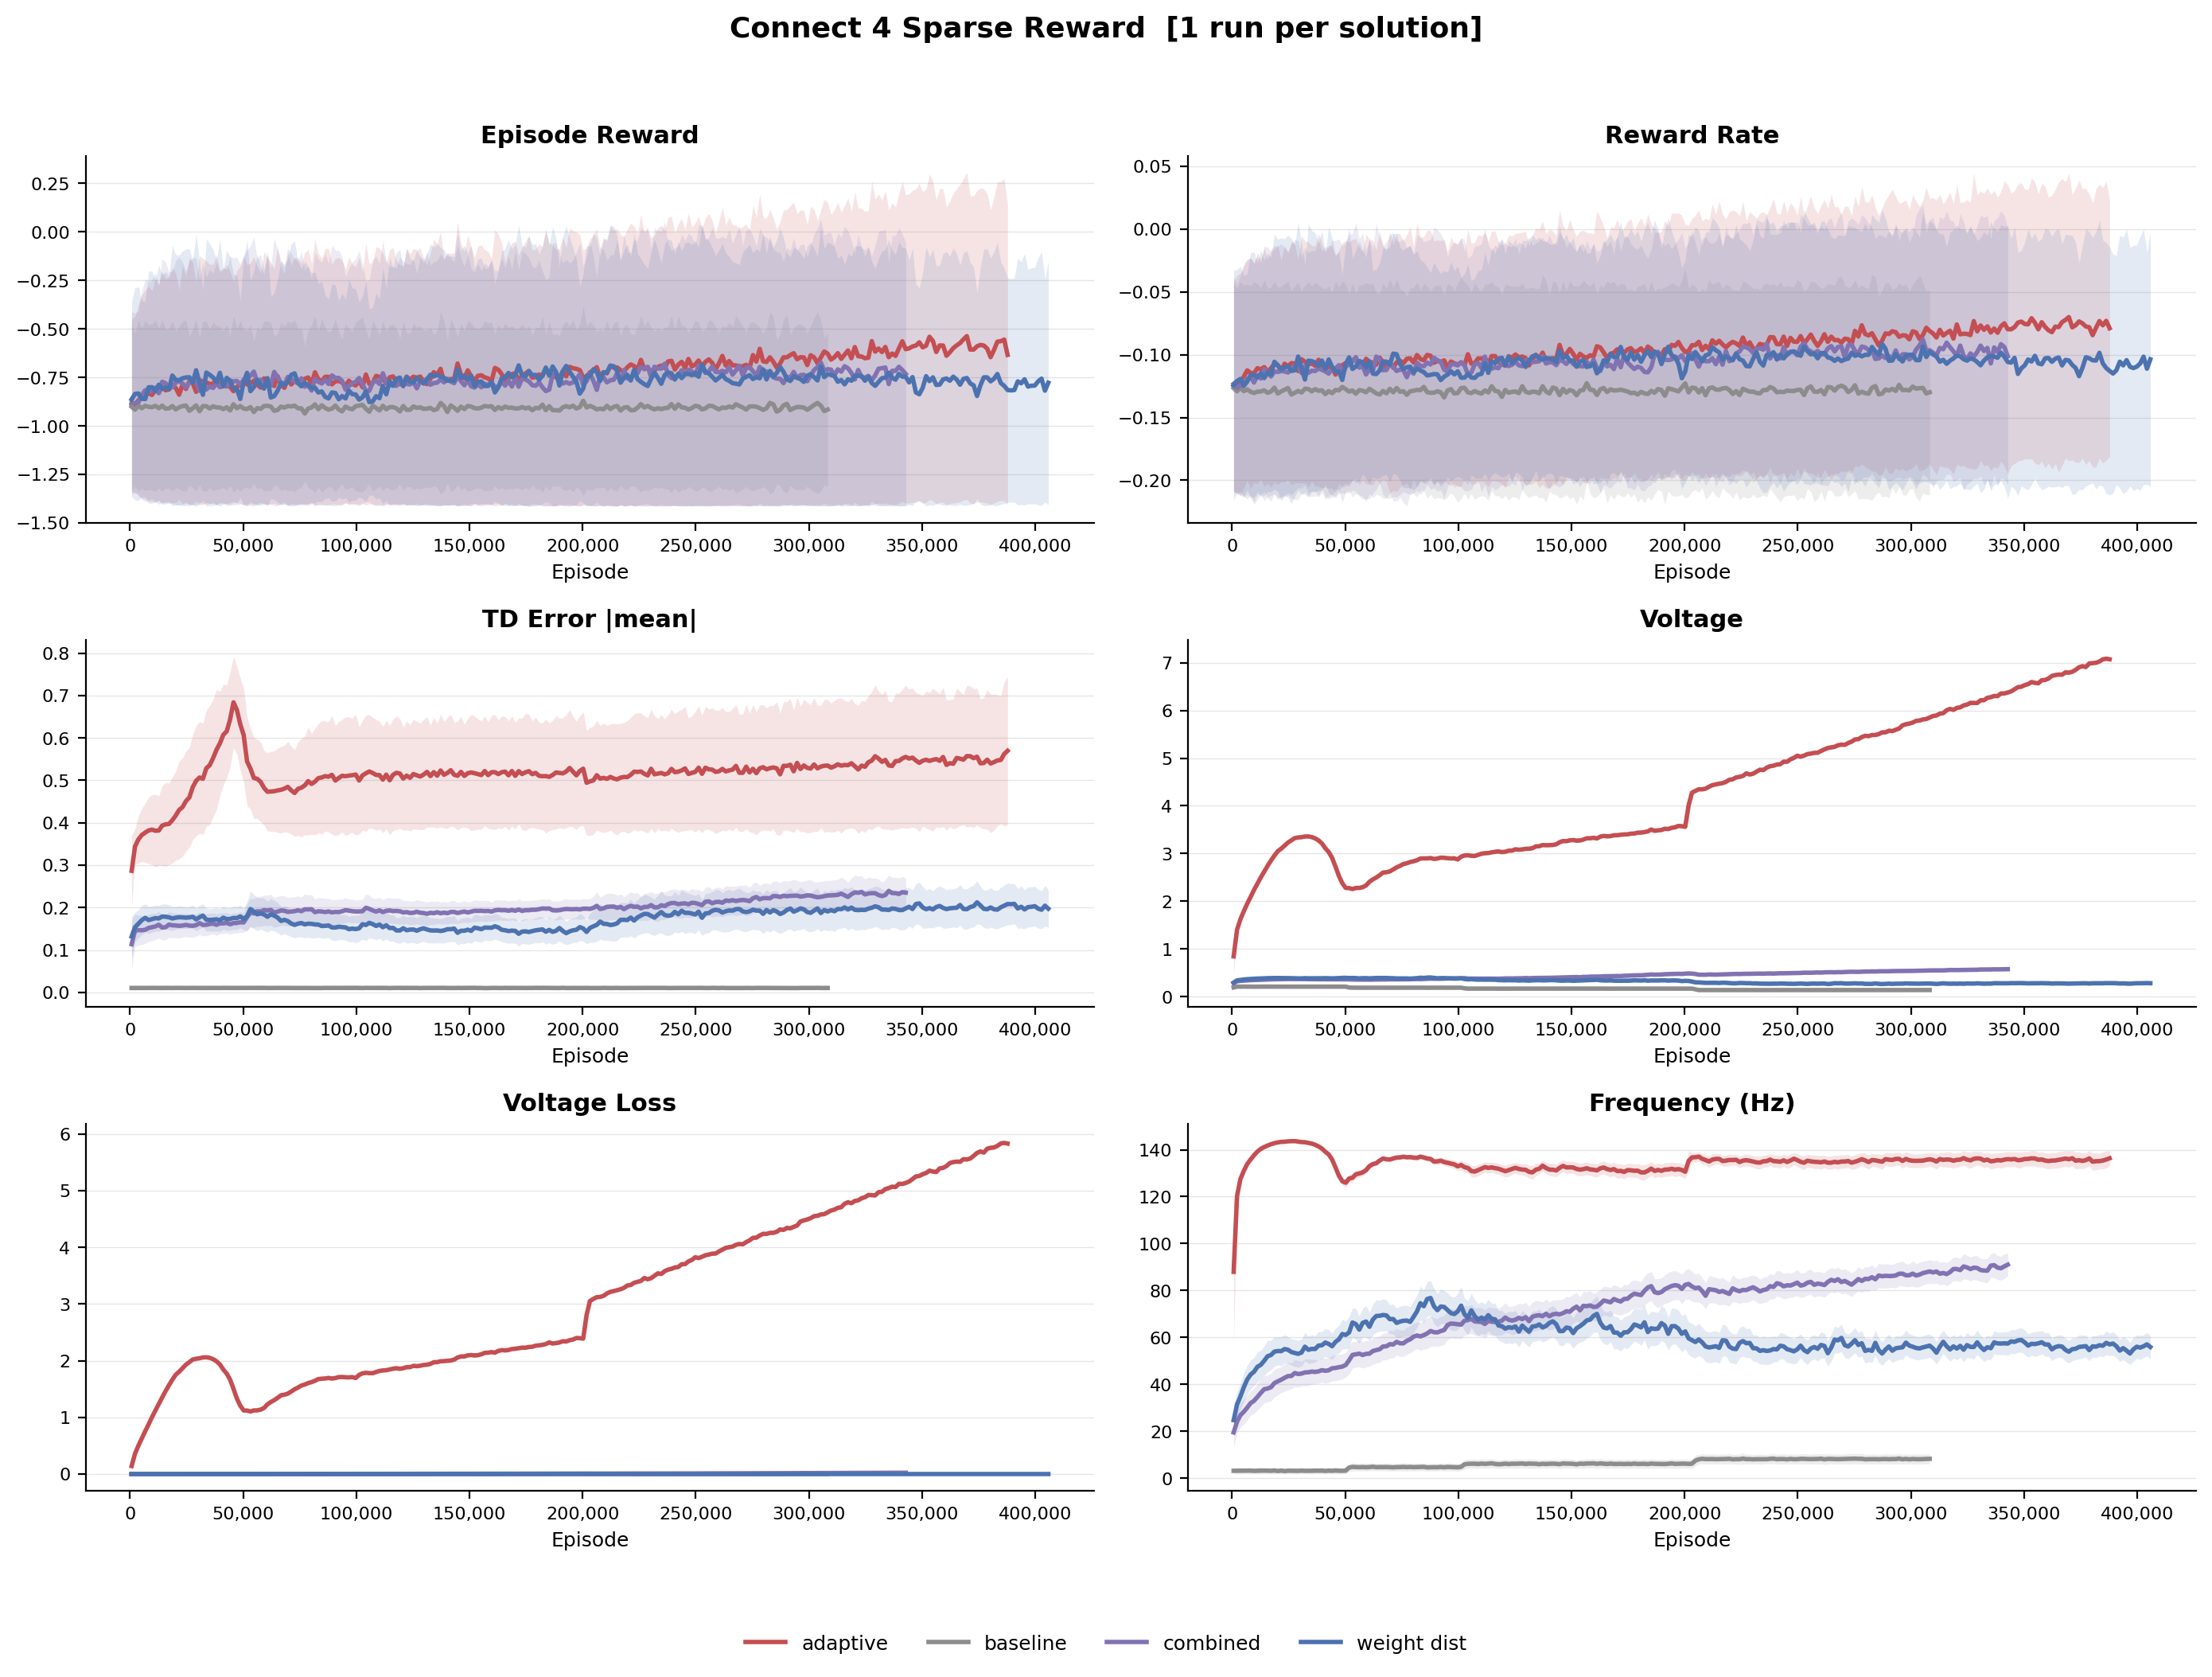
\includegraphics[width=1.0\textwidth]{images/comparison_misc_1_runs.png}
    \caption[Connect Four with sparse reward]{Training on Connect Four with a sparse terminal
    reward, comparing adaptive e-prop (red), \emph{weight dist} (blue), \emph{combined} (purple),
    and the \emph{baseline} (grey). One run per configuration; the six standard metrics are shown
    over roughly $400{,}000$ episodes. No configuration reaches a positive episode reward or reward
    rate. Adaptive e-prop shows a slight upward trend in both performance metrics, but with steadily
    growing voltage, voltage loss, and TD error, while the baseline remains essentially inert.}
    \label{fig:connect-four}
\end{figure}

None of the rules learns to play the task well, episode reward and reward rate remain negative
throughout training for every configuration. A consistent ordering nonetheless emerges in both
performance panels: adaptive e-prop sits highest and shows a slow but visible upward trend in episode
reward and reward rate, the distributed variants \emph{weight dist} and \emph{combined} follow close
behind and roughly flat, and the \emph{baseline} remains lowest and essentially flat.
The spiking-dynamics panels make clear that whatever progress adaptive e-prop makes comes at the cost
of increasingly pathological internal activity. Its membrane voltage and voltage loss do not stabilize
but climb steadily throughout training, reaching values far above any seen elsewhere in this chapter
(a voltage of around seven and a comparable voltage loss), and its mean absolute TD error sits at a
very high level, roughly an order of magnitude above the other rules. Its firing frequency saturates early in a high band around $140$~Hz. The \emph{baseline}, at the opposite extreme, is effectively
inert, its TD error stays near zero, its voltage and voltage loss remain flat and low, and its firing
rate is close to silence, the signature of a network that is not meaningfully learning a value
function or driving its neurons at all. The variants \emph{weight dist} and \emph{combined} occupy the middle
ground, with low and stable voltage and voltage loss and intermediate firing rates that drift upward
modestly, \emph{combined} rising to a higher frequency than \emph{weight dist}.

This is not a strong result, and we present it mainly to show that tasks of this kind, with a sparse
terminal reward and a long credit-assignment path, are hard for all of the learning rules considered:
none reaches a positive reward within the budget tested. What it does suggest is that adaptive e-prop
retains an advantage in learning the policy over the distributed variants even here, as it is the only
rule with a clear upward trend in episode reward and reward rate, albeit while its voltage, voltage
loss, and TD error grow steadily.

\section{Summary of the Experiments}
\label{sec:experiments-summary}

This section condenses the chapter into the messages a reader should retain.
The takeaways below are the substantive findings; the separate reading guide that follows explains
how confidently each should be held and addresses the recurring caveats.

\subsection*{Key takeaways}

\begin{itemize}
  \item \textbf{Metrics.} In the continuing, no-reset setup the operative objective is closer to the
  reward rate than to per-episode return; the two must be read together, as they can even move in
  opposite directions.
  \item \textbf{Objective horizon.} The episodic vs.\ continuing gap is set by $\gamma$, not
  $\lambda$: large at $\gamma=0.99$, nearly gone at $\gamma=0.5$. $\gamma$ fixes \emph{what} is
  optimized; $\lambda$ only sets the credit-assignment window.
  \item \textbf{Best rule on Snake.} \emph{symmetric} e-prop is the strongest single configuration,
  with the healthiest dynamics, but it collapses once the per-head field layers lengthen the causal
  path, because its feedback is tied to the output weights.
  \item \textbf{Best distributed optimizer.} Among the distributed variants, \emph{weight dist}
  optimizes best, in particular shared-postsynaptic-noise formulation.
  \item \textbf{The pseudo-derivative $\psi$ is essential.} Removing the heuristic surrogate factor
  $\psi^t_j$ (\emph{weight dist no heuristic}) collapses performance and lets the membrane voltage
  diverge (Section~\ref{sec:snake_comparison}); $\psi$ is not optional for these rules to work.
  \item \textbf{Adaptive and distributed are qualitatively different learners.} They differ less in
  final score than in \emph{how} they learn, in both spiking dynamics and the time-course of
  training. Concretely:
  \begin{itemize}
    \item \emph{Adaptive $\rightarrow$ pathological dynamics:} most prone to runaway voltage,
    voltage loss, and high firing rates, increasingly so as the causal path lengthens.
    \item \emph{Distributed $\rightarrow$ better value functions:} more stable, better-structured
    value estimates and well-regulated dynamics.
    \item \emph{Adaptive $\rightarrow$ policy edge:} on the two long-running examples (the extended
    five-layer network, Figures~\ref{fig:snake-extended-perstep}
    and~\ref{fig:snake-extended-perepisode}, and Connect Four, Section~\ref{sec:connect_four}) it is
    the only rule that keeps improving the policy, despite its noisier value estimates.
    \item \emph{Depth is a budget artifact:} at a fixed budget distributed e-prop looks more
    depth-robust, but with longer training adaptive starts slowly (feedback alignment) and then
    overtakes the distributed variants, which plateau early (Section~\ref{sec:snake_comparison}).
    \item \emph{Distributed tolerates model variations:} they could cope better with changes to the neuron
    model, e.g.\ the no-integration-during-refractory variant
    (Section~\ref{subsec:no_refractory_integration}).
  \end{itemize}
  \item \textbf{Combination adds little.} The hybrid \emph{combined} rule does not clearly
  outperform its parts, and is surprisingly the weakest on the deep per-episode run despite a strong
  showing in the one-layer comparison.
  
  \item \textbf{Update schedule.}Per-episode updates clearly help both rules on the deep (5-layer) network in Snake. On Pac-Man and Connect Four we did not run the per-episode/per-step comparison directly, though we informally observed that per-action updates tended to collapse on these tasks; we leave a systematic comparison for future work
  
  \item \textbf{regularization.} Voltage regularization works well because it is local; frequency
  regularization is harder; too much regularization strength degrades task performance.
  \item \textbf{Lambda robustness.} Neither rule is uniformly more $\lambda$-robust: distributed
  e-prop tolerates a wider $\lambda$ range on Pac-Man but shows two distinct failure modes at large
  $\lambda$ (runaway high activity vs.\ excessive silence), and the ordering is reversed on Snake.
  \item \textbf{Why deep nets fail (qualitative).} Deeper \emph{weight dist} networks develop flat,
  unstructured value estimates and near-deterministic policies, i.e.\ they lose exploration.
  \item \textbf{Hardest task: Connect Four (sparse reward).} Hard for every rule and solved by none;
  consistent with the policy-edge point above, adaptive e-prop shows the only positive learning
  trend.
  \item \textbf{The model assumptions are sound.} The \emph{baseline}, in which the recurrent
  weights are not trained, stays essentially flat in every experiment where it was tested, so the
  recurrent learning these rules perform is doing real work, the gains are not an artifact of the
  architecture or readout alone.
    \item \textbf{High firing rates are pervasive.} All learning rules across all
    tasks converge to firing rates of roughly 130 to 170~Hz, far above both the
    biological range and the $F^* = 10$~Hz regularization target. Our hypothesis is
    that the tasks studied require near-constant firing for reactive value and
    policy estimation, and that without a clear learning signal the dynamics tend
    to drift toward saturated activity.
\end{itemize}
